% Options for packages loaded elsewhere
\PassOptionsToPackage{unicode}{hyperref}
\PassOptionsToPackage{hyphens}{url}
\PassOptionsToPackage{dvipsnames,svgnames,x11names}{xcolor}
%
\documentclass[
  letterpaper,
  DIV=11,
  numbers=noendperiod]{scrreprt}

\usepackage{amsmath,amssymb}
\usepackage{iftex}
\ifPDFTeX
  \usepackage[T1]{fontenc}
  \usepackage[utf8]{inputenc}
  \usepackage{textcomp} % provide euro and other symbols
\else % if luatex or xetex
  \usepackage{unicode-math}
  \defaultfontfeatures{Scale=MatchLowercase}
  \defaultfontfeatures[\rmfamily]{Ligatures=TeX,Scale=1}
\fi
\usepackage{lmodern}
\ifPDFTeX\else  
    % xetex/luatex font selection
\fi
% Use upquote if available, for straight quotes in verbatim environments
\IfFileExists{upquote.sty}{\usepackage{upquote}}{}
\IfFileExists{microtype.sty}{% use microtype if available
  \usepackage[]{microtype}
  \UseMicrotypeSet[protrusion]{basicmath} % disable protrusion for tt fonts
}{}
\makeatletter
\@ifundefined{KOMAClassName}{% if non-KOMA class
  \IfFileExists{parskip.sty}{%
    \usepackage{parskip}
  }{% else
    \setlength{\parindent}{0pt}
    \setlength{\parskip}{6pt plus 2pt minus 1pt}}
}{% if KOMA class
  \KOMAoptions{parskip=half}}
\makeatother
\usepackage{xcolor}
\usepackage{svg}
\setlength{\emergencystretch}{3em} % prevent overfull lines
\setcounter{secnumdepth}{5}
% Make \paragraph and \subparagraph free-standing
\makeatletter
\ifx\paragraph\undefined\else
  \let\oldparagraph\paragraph
  \renewcommand{\paragraph}{
    \@ifstar
      \xxxParagraphStar
      \xxxParagraphNoStar
  }
  \newcommand{\xxxParagraphStar}[1]{\oldparagraph*{#1}\mbox{}}
  \newcommand{\xxxParagraphNoStar}[1]{\oldparagraph{#1}\mbox{}}
\fi
\ifx\subparagraph\undefined\else
  \let\oldsubparagraph\subparagraph
  \renewcommand{\subparagraph}{
    \@ifstar
      \xxxSubParagraphStar
      \xxxSubParagraphNoStar
  }
  \newcommand{\xxxSubParagraphStar}[1]{\oldsubparagraph*{#1}\mbox{}}
  \newcommand{\xxxSubParagraphNoStar}[1]{\oldsubparagraph{#1}\mbox{}}
\fi
\makeatother

\usepackage{color}
\usepackage{fancyvrb}
\newcommand{\VerbBar}{|}
\newcommand{\VERB}{\Verb[commandchars=\\\{\}]}
\DefineVerbatimEnvironment{Highlighting}{Verbatim}{commandchars=\\\{\}}
% Add ',fontsize=\small' for more characters per line
\usepackage{framed}
\definecolor{shadecolor}{RGB}{241,243,245}
\newenvironment{Shaded}{\begin{snugshade}}{\end{snugshade}}
\newcommand{\AlertTok}[1]{\textcolor[rgb]{0.68,0.00,0.00}{#1}}
\newcommand{\AnnotationTok}[1]{\textcolor[rgb]{0.37,0.37,0.37}{#1}}
\newcommand{\AttributeTok}[1]{\textcolor[rgb]{0.40,0.45,0.13}{#1}}
\newcommand{\BaseNTok}[1]{\textcolor[rgb]{0.68,0.00,0.00}{#1}}
\newcommand{\BuiltInTok}[1]{\textcolor[rgb]{0.00,0.23,0.31}{#1}}
\newcommand{\CharTok}[1]{\textcolor[rgb]{0.13,0.47,0.30}{#1}}
\newcommand{\CommentTok}[1]{\textcolor[rgb]{0.37,0.37,0.37}{#1}}
\newcommand{\CommentVarTok}[1]{\textcolor[rgb]{0.37,0.37,0.37}{\textit{#1}}}
\newcommand{\ConstantTok}[1]{\textcolor[rgb]{0.56,0.35,0.01}{#1}}
\newcommand{\ControlFlowTok}[1]{\textcolor[rgb]{0.00,0.23,0.31}{\textbf{#1}}}
\newcommand{\DataTypeTok}[1]{\textcolor[rgb]{0.68,0.00,0.00}{#1}}
\newcommand{\DecValTok}[1]{\textcolor[rgb]{0.68,0.00,0.00}{#1}}
\newcommand{\DocumentationTok}[1]{\textcolor[rgb]{0.37,0.37,0.37}{\textit{#1}}}
\newcommand{\ErrorTok}[1]{\textcolor[rgb]{0.68,0.00,0.00}{#1}}
\newcommand{\ExtensionTok}[1]{\textcolor[rgb]{0.00,0.23,0.31}{#1}}
\newcommand{\FloatTok}[1]{\textcolor[rgb]{0.68,0.00,0.00}{#1}}
\newcommand{\FunctionTok}[1]{\textcolor[rgb]{0.28,0.35,0.67}{#1}}
\newcommand{\ImportTok}[1]{\textcolor[rgb]{0.00,0.46,0.62}{#1}}
\newcommand{\InformationTok}[1]{\textcolor[rgb]{0.37,0.37,0.37}{#1}}
\newcommand{\KeywordTok}[1]{\textcolor[rgb]{0.00,0.23,0.31}{\textbf{#1}}}
\newcommand{\NormalTok}[1]{\textcolor[rgb]{0.00,0.23,0.31}{#1}}
\newcommand{\OperatorTok}[1]{\textcolor[rgb]{0.37,0.37,0.37}{#1}}
\newcommand{\OtherTok}[1]{\textcolor[rgb]{0.00,0.23,0.31}{#1}}
\newcommand{\PreprocessorTok}[1]{\textcolor[rgb]{0.68,0.00,0.00}{#1}}
\newcommand{\RegionMarkerTok}[1]{\textcolor[rgb]{0.00,0.23,0.31}{#1}}
\newcommand{\SpecialCharTok}[1]{\textcolor[rgb]{0.37,0.37,0.37}{#1}}
\newcommand{\SpecialStringTok}[1]{\textcolor[rgb]{0.13,0.47,0.30}{#1}}
\newcommand{\StringTok}[1]{\textcolor[rgb]{0.13,0.47,0.30}{#1}}
\newcommand{\VariableTok}[1]{\textcolor[rgb]{0.07,0.07,0.07}{#1}}
\newcommand{\VerbatimStringTok}[1]{\textcolor[rgb]{0.13,0.47,0.30}{#1}}
\newcommand{\WarningTok}[1]{\textcolor[rgb]{0.37,0.37,0.37}{\textit{#1}}}

\providecommand{\tightlist}{%
  \setlength{\itemsep}{0pt}\setlength{\parskip}{0pt}}\usepackage{longtable,booktabs,array}
\usepackage{calc} % for calculating minipage widths
% Correct order of tables after \paragraph or \subparagraph
\usepackage{etoolbox}
\makeatletter
\patchcmd\longtable{\par}{\if@noskipsec\mbox{}\fi\par}{}{}
\makeatother
% Allow footnotes in longtable head/foot
\IfFileExists{footnotehyper.sty}{\usepackage{footnotehyper}}{\usepackage{footnote}}
\makesavenoteenv{longtable}
\usepackage{graphicx}
\makeatletter
\newsavebox\pandoc@box
\newcommand*\pandocbounded[1]{% scales image to fit in text height/width
  \sbox\pandoc@box{#1}%
  \Gscale@div\@tempa{\textheight}{\dimexpr\ht\pandoc@box+\dp\pandoc@box\relax}%
  \Gscale@div\@tempb{\linewidth}{\wd\pandoc@box}%
  \ifdim\@tempb\p@<\@tempa\p@\let\@tempa\@tempb\fi% select the smaller of both
  \ifdim\@tempa\p@<\p@\scalebox{\@tempa}{\usebox\pandoc@box}%
  \else\usebox{\pandoc@box}%
  \fi%
}
% Set default figure placement to htbp
\def\fps@figure{htbp}
\makeatother
% definitions for citeproc citations
\NewDocumentCommand\citeproctext{}{}
\NewDocumentCommand\citeproc{mm}{%
  \begingroup\def\citeproctext{#2}\cite{#1}\endgroup}
\makeatletter
 % allow citations to break across lines
 \let\@cite@ofmt\@firstofone
 % avoid brackets around text for \cite:
 \def\@biblabel#1{}
 \def\@cite#1#2{{#1\if@tempswa , #2\fi}}
\makeatother
\newlength{\cslhangindent}
\setlength{\cslhangindent}{1.5em}
\newlength{\csllabelwidth}
\setlength{\csllabelwidth}{3em}
\newenvironment{CSLReferences}[2] % #1 hanging-indent, #2 entry-spacing
 {\begin{list}{}{%
  \setlength{\itemindent}{0pt}
  \setlength{\leftmargin}{0pt}
  \setlength{\parsep}{0pt}
  % turn on hanging indent if param 1 is 1
  \ifodd #1
   \setlength{\leftmargin}{\cslhangindent}
   \setlength{\itemindent}{-1\cslhangindent}
  \fi
  % set entry spacing
  \setlength{\itemsep}{#2\baselineskip}}}
 {\end{list}}
\usepackage{calc}
\newcommand{\CSLBlock}[1]{\hfill\break\parbox[t]{\linewidth}{\strut\ignorespaces#1\strut}}
\newcommand{\CSLLeftMargin}[1]{\parbox[t]{\csllabelwidth}{\strut#1\strut}}
\newcommand{\CSLRightInline}[1]{\parbox[t]{\linewidth - \csllabelwidth}{\strut#1\strut}}
\newcommand{\CSLIndent}[1]{\hspace{\cslhangindent}#1}

\KOMAoption{captions}{tableheading}
\makeatletter
\@ifpackageloaded{tcolorbox}{}{\usepackage[skins,breakable]{tcolorbox}}
\@ifpackageloaded{fontawesome5}{}{\usepackage{fontawesome5}}
\definecolor{quarto-callout-color}{HTML}{909090}
\definecolor{quarto-callout-note-color}{HTML}{0758E5}
\definecolor{quarto-callout-important-color}{HTML}{CC1914}
\definecolor{quarto-callout-warning-color}{HTML}{EB9113}
\definecolor{quarto-callout-tip-color}{HTML}{00A047}
\definecolor{quarto-callout-caution-color}{HTML}{FC5300}
\definecolor{quarto-callout-color-frame}{HTML}{acacac}
\definecolor{quarto-callout-note-color-frame}{HTML}{4582ec}
\definecolor{quarto-callout-important-color-frame}{HTML}{d9534f}
\definecolor{quarto-callout-warning-color-frame}{HTML}{f0ad4e}
\definecolor{quarto-callout-tip-color-frame}{HTML}{02b875}
\definecolor{quarto-callout-caution-color-frame}{HTML}{fd7e14}
\makeatother
\makeatletter
\@ifpackageloaded{bookmark}{}{\usepackage{bookmark}}
\makeatother
\makeatletter
\@ifpackageloaded{caption}{}{\usepackage{caption}}
\AtBeginDocument{%
\ifdefined\contentsname
  \renewcommand*\contentsname{Table of contents}
\else
  \newcommand\contentsname{Table of contents}
\fi
\ifdefined\listfigurename
  \renewcommand*\listfigurename{List of Figures}
\else
  \newcommand\listfigurename{List of Figures}
\fi
\ifdefined\listtablename
  \renewcommand*\listtablename{List of Tables}
\else
  \newcommand\listtablename{List of Tables}
\fi
\ifdefined\figurename
  \renewcommand*\figurename{Figure}
\else
  \newcommand\figurename{Figure}
\fi
\ifdefined\tablename
  \renewcommand*\tablename{Table}
\else
  \newcommand\tablename{Table}
\fi
}
\@ifpackageloaded{float}{}{\usepackage{float}}
\floatstyle{ruled}
\@ifundefined{c@chapter}{\newfloat{codelisting}{h}{lop}}{\newfloat{codelisting}{h}{lop}[chapter]}
\floatname{codelisting}{Listing}
\newcommand*\listoflistings{\listof{codelisting}{List of Listings}}
\makeatother
\makeatletter
\makeatother
\makeatletter
\@ifpackageloaded{caption}{}{\usepackage{caption}}
\@ifpackageloaded{subcaption}{}{\usepackage{subcaption}}
\makeatother

\usepackage{bookmark}

\IfFileExists{xurl.sty}{\usepackage{xurl}}{} % add URL line breaks if available
\urlstyle{same} % disable monospaced font for URLs
\hypersetup{
  pdftitle={Shell genomics},
  colorlinks=true,
  linkcolor={blue},
  filecolor={Maroon},
  citecolor={Blue},
  urlcolor={Blue},
  pdfcreator={LaTeX via pandoc}}


\title{Shell genomics}
\author{}
\date{2023-11-15}

\begin{document}
\maketitle

\renewcommand*\contentsname{Table of contents}
{
\hypersetup{linkcolor=}
\setcounter{tocdepth}{2}
\tableofcontents
}

\bookmarksetup{startatroot}

\chapter*{Preface}\label{preface}
\addcontentsline{toc}{chapter}{Preface}

\markboth{Preface}{Preface}

The content of this workshop is based on the material by the Data
Carpentry: Introduction to the shell for genomics data (Becker et al.
2019).

Command line interface (CLI) and graphic user interface (GUI) are
different ways of interacting with a computer's operating system. They
have different pros and cons. Most people are familiar with the GUI as
it is the default interface for most software, particularly on Windows
and Mac OS. When using the GUI, you see visual representations of files,
folders, applications etc. When using the CLI, you work largely with
text representations of files, folders, input and output etc. The shell
is a program that presents a command line interface that allows you to
control your computer by typing instructions with a keyboard.

There are several reasons to learn how to use the CLI:

\begin{itemize}
\item
  For most bioinformatics tools, there are no graphical interfaces. If
  you want to work in metagenomics or genomics you're going to need to
  use the CLI/shell.
\item
  The shell gives you power. The command line allows you to work more
  efficiently. Tasks that are repetitive (e.g.~renaming hundreds of
  files) can be automated. Tasks that are tedious (e.g.~testing a range
  of input parameters) can be simplified.
\item
  To use remote computers or cloud computing, you need to use the shell.
\end{itemize}

\section*{\texorpdfstring{\textbf{Schedule}}{Schedule}}\label{schedule}
\addcontentsline{toc}{section}{\textbf{Schedule}}

\markright{\textbf{Schedule}}

\begin{longtable}[]{@{}
  >{\raggedright\arraybackslash}p{(\linewidth - 4\tabcolsep) * \real{0.0597}}
  >{\raggedright\arraybackslash}p{(\linewidth - 4\tabcolsep) * \real{0.3284}}
  >{\raggedright\arraybackslash}p{(\linewidth - 4\tabcolsep) * \real{0.6045}}@{}}
\toprule\noalign{}
\begin{minipage}[b]{\linewidth}\raggedright
\end{minipage} & \begin{minipage}[b]{\linewidth}\raggedright
Setup
\end{minipage} & \begin{minipage}[b]{\linewidth}\raggedright
Download files required for the lesson
\end{minipage} \\
\midrule\noalign{}
\endhead
\bottomrule\noalign{}
\endlastfoot
00:00 & 1. Introducing the Shell &
\begin{minipage}[t]{\linewidth}\raggedright
What is a command shell and why would I use one?\\
How can I move around on my computer?\\
How can I see what files and directories I have?\\
How can I specify the location of a file or directory on my
computer?\strut
\end{minipage} \\
00:30 & 2. Navigating Files and Directories &
\begin{minipage}[t]{\linewidth}\raggedright
How can I perform operations on files outside of my working directory?\\
What are some navigational shortcuts I can use to make my work more
efficient?\strut
\end{minipage} \\
01:20 & 3. Working with Files and Directories &
\begin{minipage}[t]{\linewidth}\raggedright
How can I view and search file contents?\\
How can I create, copy and delete files and directories?\\
How can I control who has permission to modify a file?\\
How can I repeat recently used commands?\strut
\end{minipage} \\
02:05 & 4. Redirection & \begin{minipage}[t]{\linewidth}\raggedright
How can I search within files?\\
How can I combine existing commands to do new things?\strut
\end{minipage} \\
02:50 & 5. Writing Scripts and Working with Data & How can we automate a
commonly used set of commands? \\
03:30 & 6. Project Organization &
\begin{minipage}[t]{\linewidth}\raggedright
How can I organize my file system for a new bioinformatics project?\\
How can I document my work?\strut
\end{minipage} \\
04:00 & Finish & \\
\end{longtable}

The actual schedule may vary slightly depending on the topics and
exercises chosen by the instructor.

\bookmarksetup{startatroot}

\chapter{Introducing the shell}\label{sec-introducing-the-shell}

\begin{tcolorbox}[enhanced jigsaw, opacitybacktitle=0.6, colback=white, coltitle=black, opacityback=0, rightrule=.15mm, toptitle=1mm, toprule=.15mm, bottomtitle=1mm, colframe=quarto-callout-note-color-frame, arc=.35mm, titlerule=0mm, colbacktitle=quarto-callout-note-color!10!white, leftrule=.75mm, title={⏳ Time}, breakable, bottomrule=.15mm, left=2mm]

\begin{itemize}
\tightlist
\item
  Teaching: 20 min
\item
  Exercises: 10 min
\end{itemize}

\end{tcolorbox}

\begin{tcolorbox}[enhanced jigsaw, opacitybacktitle=0.6, colback=white, coltitle=black, opacityback=0, rightrule=.15mm, toptitle=1mm, toprule=.15mm, bottomtitle=1mm, colframe=quarto-callout-tip-color-frame, arc=.35mm, titlerule=0mm, colbacktitle=quarto-callout-tip-color!10!white, leftrule=.75mm, title={🤔 Questions}, breakable, bottomrule=.15mm, left=2mm]

\begin{itemize}
\tightlist
\item
  What is a command shell and why would I use one?
\item
  How can I move around on my computer?
\item
  How can I see what files and directories I have?
\item
  How can I specify the location of a file or directory on my computer?
\end{itemize}

\end{tcolorbox}

\begin{tcolorbox}[enhanced jigsaw, opacitybacktitle=0.6, colback=white, coltitle=black, opacityback=0, rightrule=.15mm, toptitle=1mm, toprule=.15mm, bottomtitle=1mm, colframe=quarto-callout-important-color-frame, arc=.35mm, titlerule=0mm, colbacktitle=quarto-callout-important-color!10!white, leftrule=.75mm, title={🎯 Objectives}, breakable, bottomrule=.15mm, left=2mm]

\begin{itemize}
\tightlist
\item
  Describe key reasons for learning shell.
\item
  Navigate your file system using the command line.
\item
  Access and read help files for \texttt{bash} programs and use help
  files to identify useful command options.
\item
  Demonstrate the use of tab completion, and explain its advantages.
\end{itemize}

\end{tcolorbox}

\section{What is a shell and why should I
care?}\label{what-is-a-shell-and-why-should-i-care}

A \emph{shell} is a computer program that presents a command line
interface which allows you to control your computer using commands
entered with a keyboard instead of controlling graphical user interfaces
(GUIs) with a mouse/keyboard/touchscreen combination.

There are many reasons to learn about the shell:

\begin{itemize}
\item
  Many bioinformatics tools can only be used through a command line
  interface. Many more have features and parameter options which are not
  available in the GUI. BLAST is an example. Many of the advanced
  functions are only accessible to users who know how to use a shell.
\item
  The shell makes your work less boring. In bioinformatics you often
  need to repeat tasks with a large number of files. With the shell, you
  can automate those repetitive tasks and leave you free to do more
  exciting things.
\item
  The shell makes your work less error-prone. When humans do the same
  thing a hundred different times (or even ten times), they're likely to
  make a mistake. Your computer can do the same thing a thousand times
  with no mistakes.
\item
  The shell makes your work more reproducible. When you carry out your
  work in the command-line (rather than a GUI), your computer keeps a
  record of every step that you've carried out, which you can use to
  re-do your work when you need to. It also gives you a way to
  communicate unambiguously what you've done, so that others can inspect
  or apply your process to new data.
\item
  Many bioinformatic tasks require large amounts of computing power and
  can't realistically be run on your own machine. These tasks are best
  performed using remote computers or cloud computing, which can only be
  accessed through a shell.
\end{itemize}

In this lesson you will learn how to use the command line interface to
move around in your file system.

\section{How to access the shell}\label{how-to-access-the-shell}

The Terminal is a window into which we will use to type commands in.

\subsection{Windows}\label{sec-}

If you're using Windows, you need to use a separate program to access
the shell. You can use \href{https://mobaxterm.mobatek.net/}{MobaXterm},
a terminal for Windows, that is already installed on your machine.

\begin{enumerate}
\def\labelenumi{\arabic{enumi}.}
\tightlist
\item
  Click on the MobaXterm icon on your desktop.
\item
  Select \texttt{Start\ local\ terminal}
\end{enumerate}

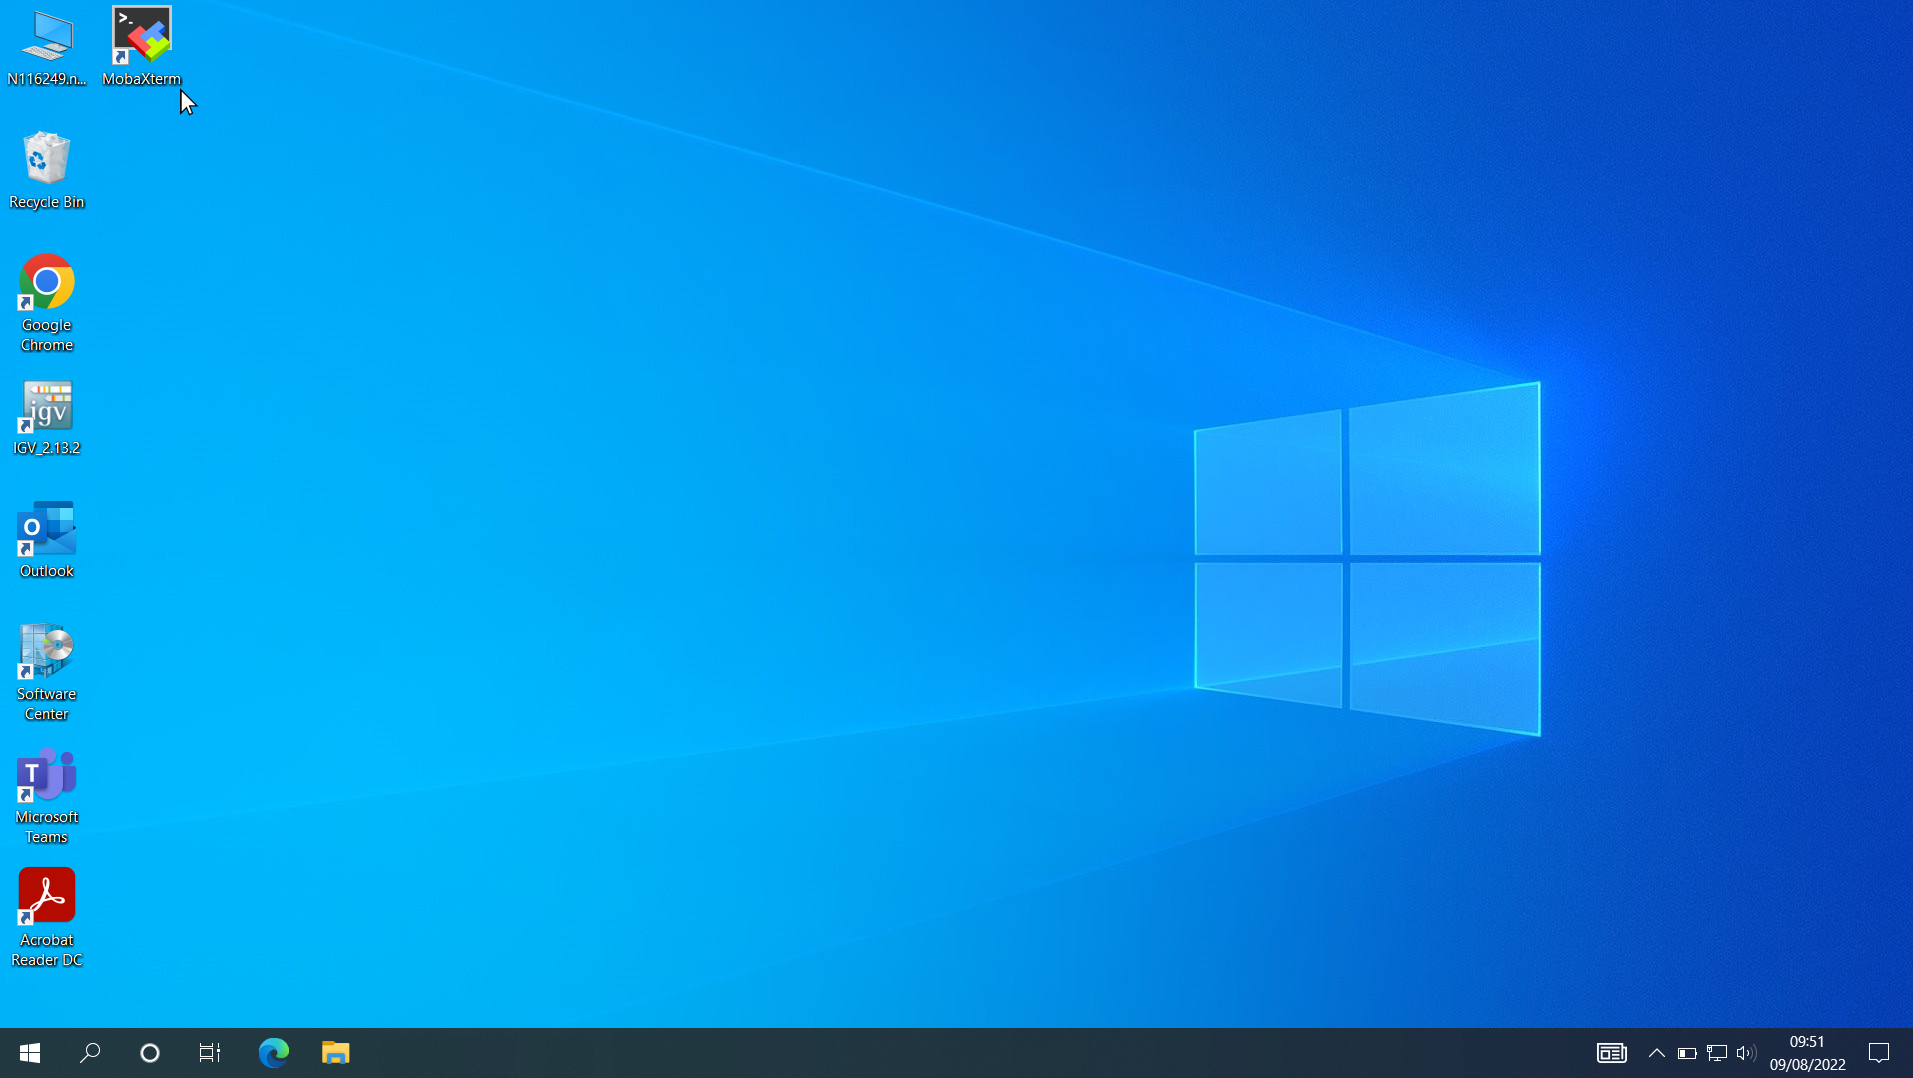
\includegraphics[width=1\linewidth,height=\textheight,keepaspectratio]{images/windows-desktop.png}

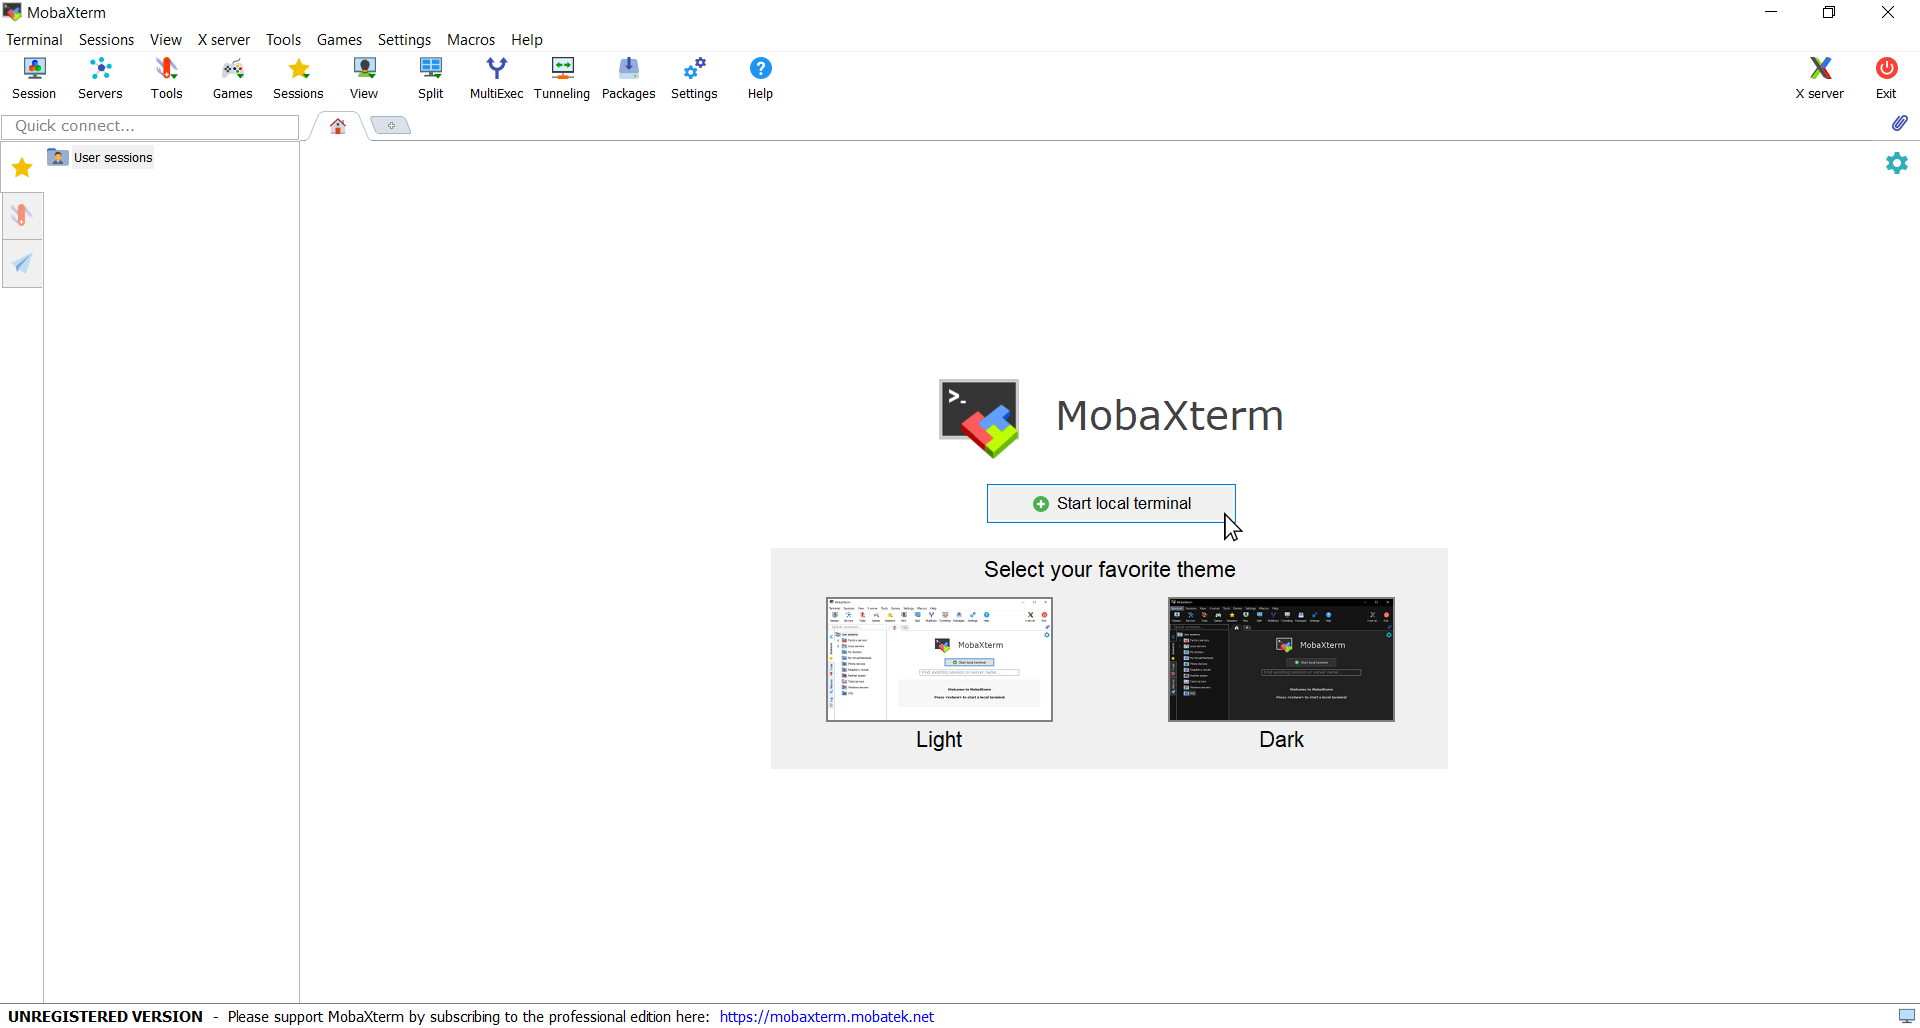
\includegraphics[width=1\linewidth,height=\textheight,keepaspectratio]{images/mobaxterm-opening.png}

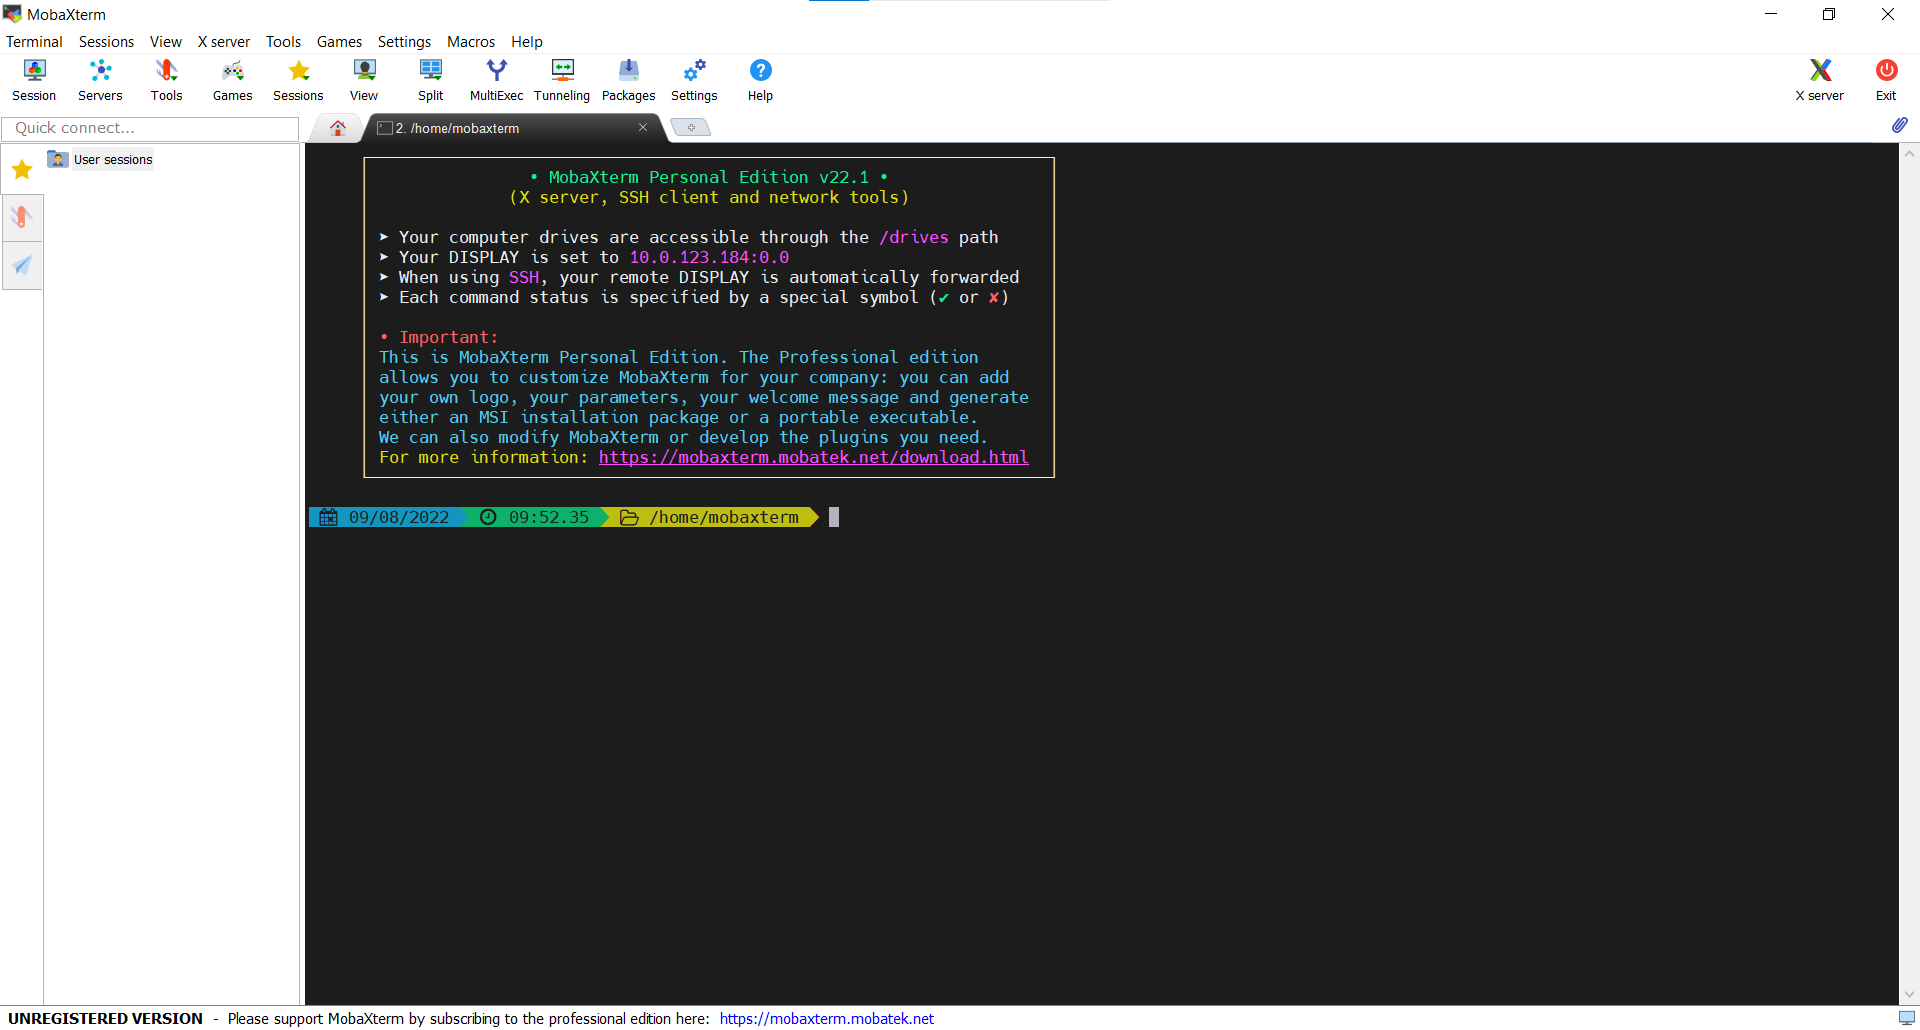
\includegraphics[width=1\linewidth,height=\textheight,keepaspectratio]{images/mobaxterm-terminal.png}

\subsection{MacOS}\label{macos}

On a Mac or Linux machine, you can access a shell through a program
called ``Terminal'', which is already available on your computer.

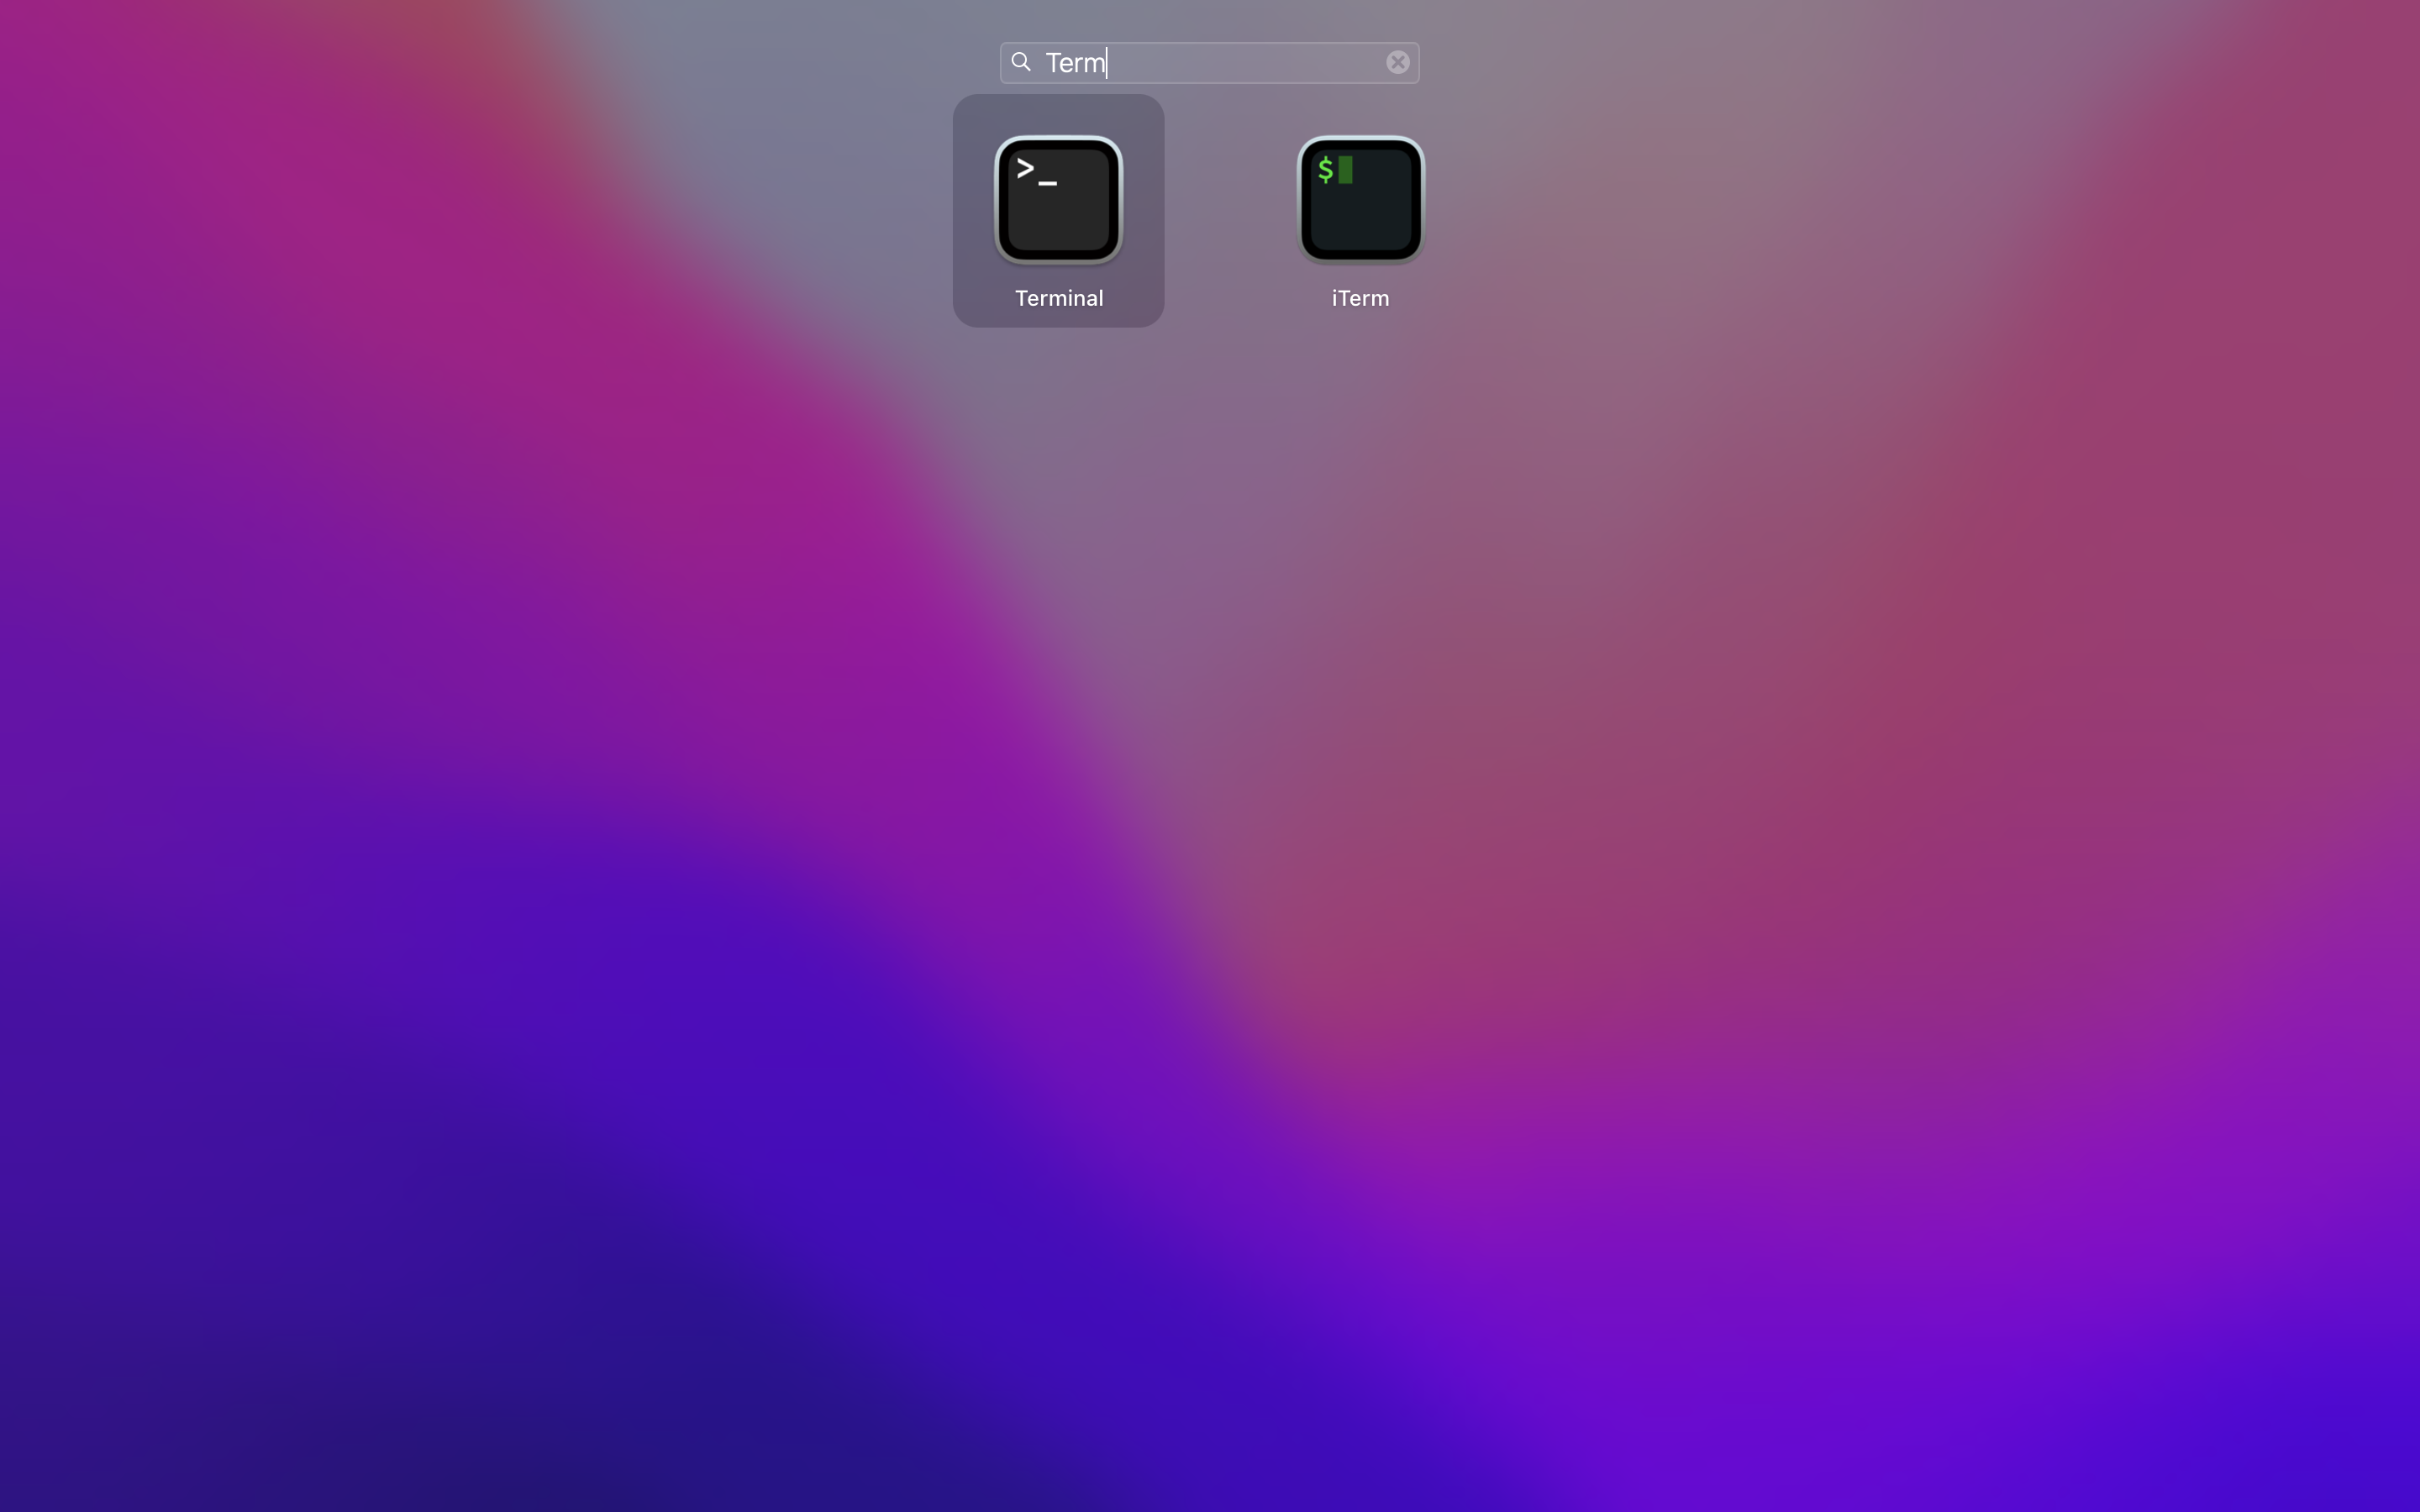
\includegraphics[width=1\linewidth,height=\textheight,keepaspectratio]{images/mac-launchpad-term.png}

\begin{figure}

\begin{minipage}{0.50\linewidth}

\begin{figure}[H]

{\centering \pandocbounded{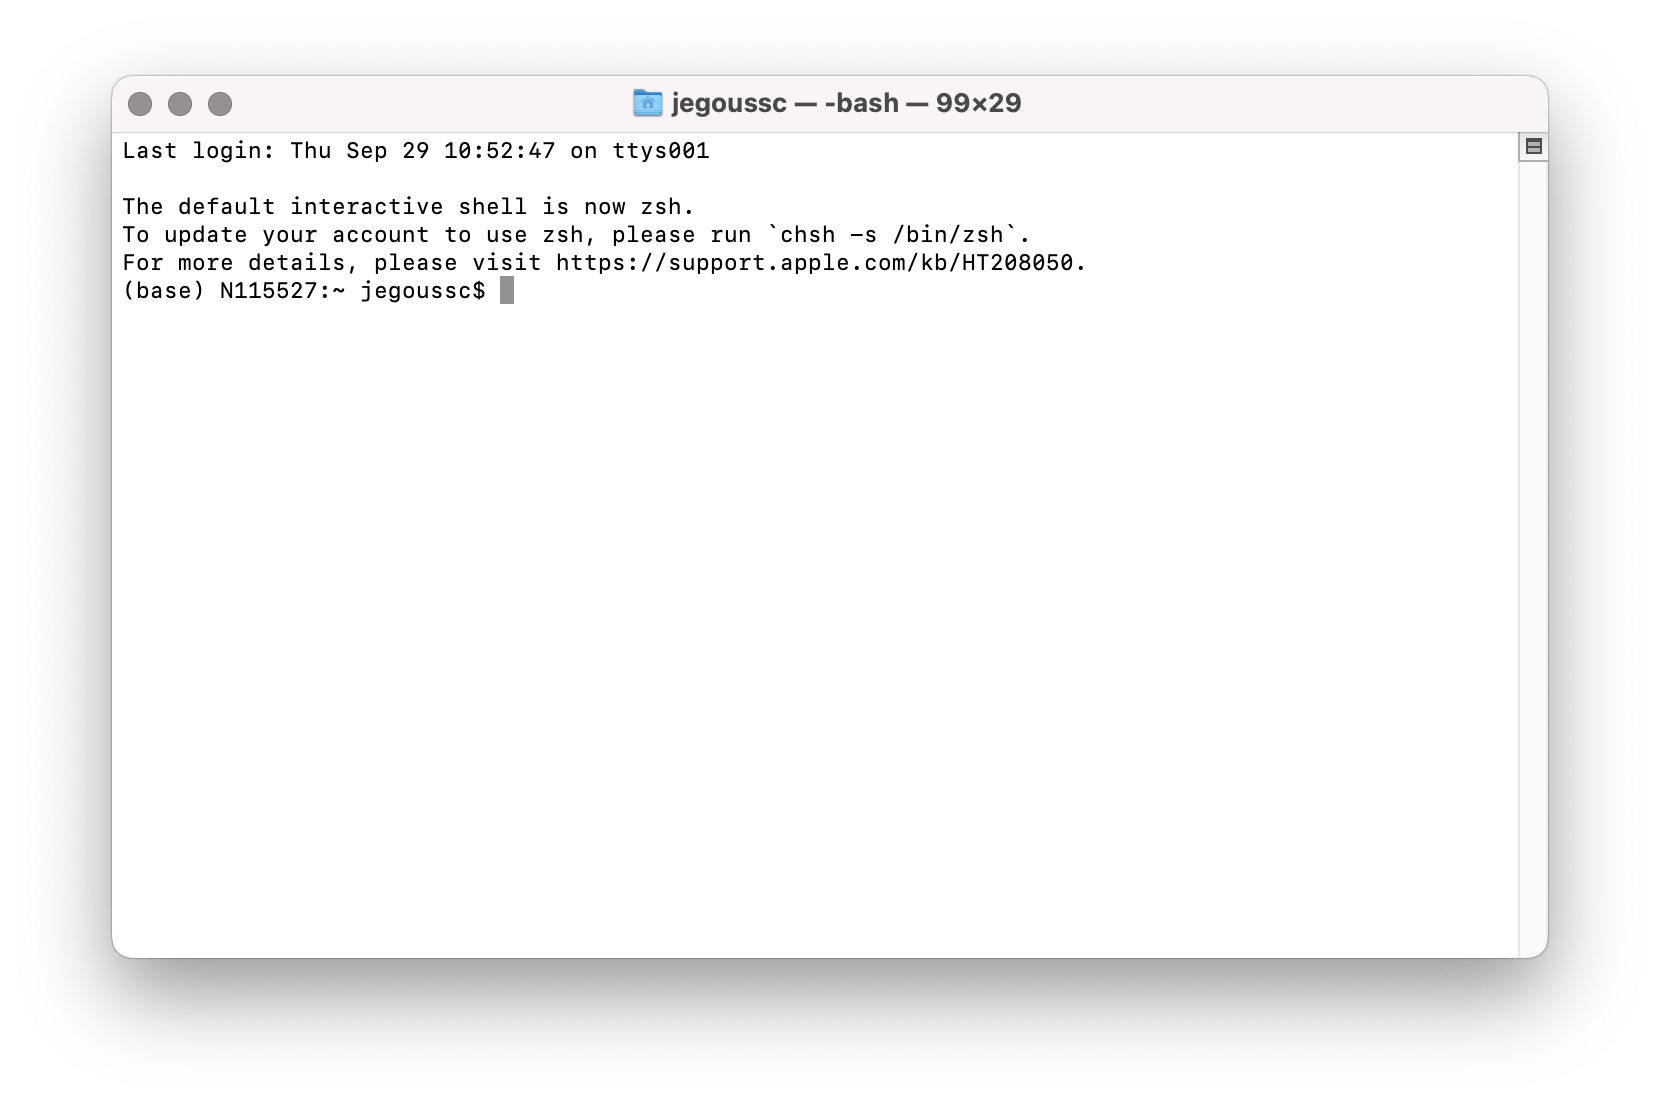
\includegraphics[keepaspectratio]{images/mac-terminal.png}}

}

\subcaption{Terminal}

\end{figure}%

\end{minipage}%
%
\begin{minipage}{0.50\linewidth}

\begin{figure}[H]

{\centering \pandocbounded{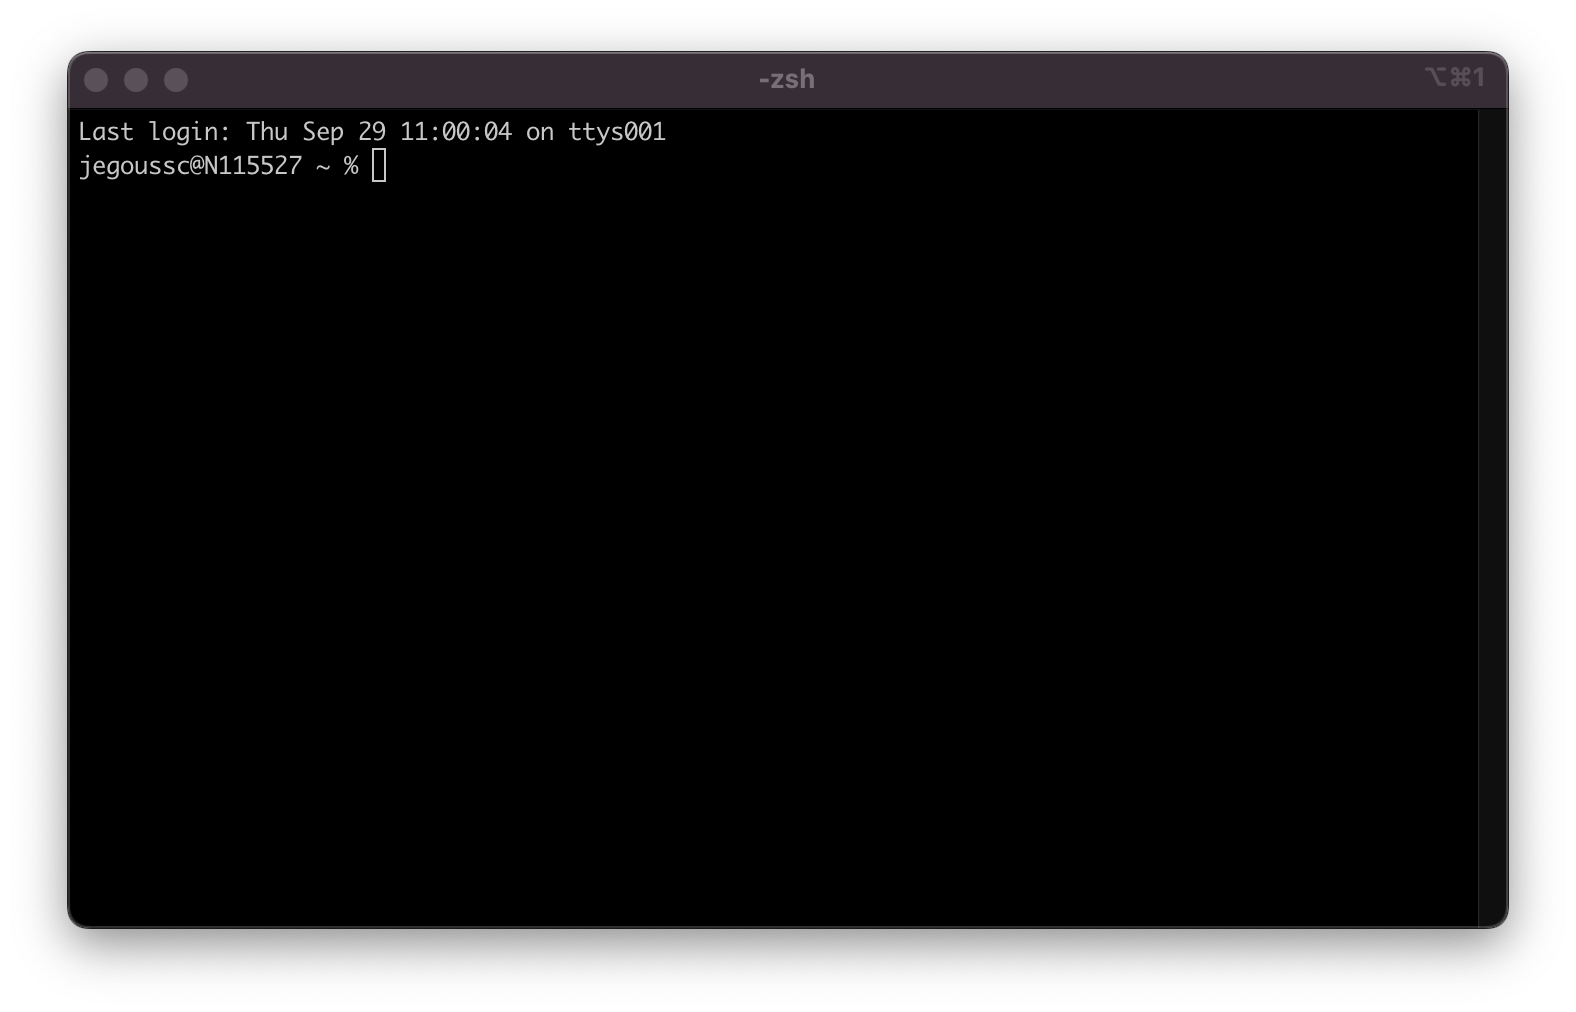
\includegraphics[keepaspectratio]{images/mac-iterm.png}}

}

\subcaption{iTerm}

\end{figure}%

\end{minipage}%

\end{figure}%

\section{How to access the remote
server}\label{how-to-access-the-remote-server}

To save time, we are going to be working on a remote server where all
the necessary data and software available. When we say a `remote sever',
we are talking about a computer that is not the one you are working on
right now. You will access the remote server where everything is
prepared for the lesson. We will learn the basics of the shell by
manipulating some data files. Some of these files are very large , and
would take time to download to your computer. We will also be using
several bioinformatic packages in later lessons and installing all of
the software would take up time even more time. A `ready-to-go' sever
let's us focus on learning.

\pandocbounded{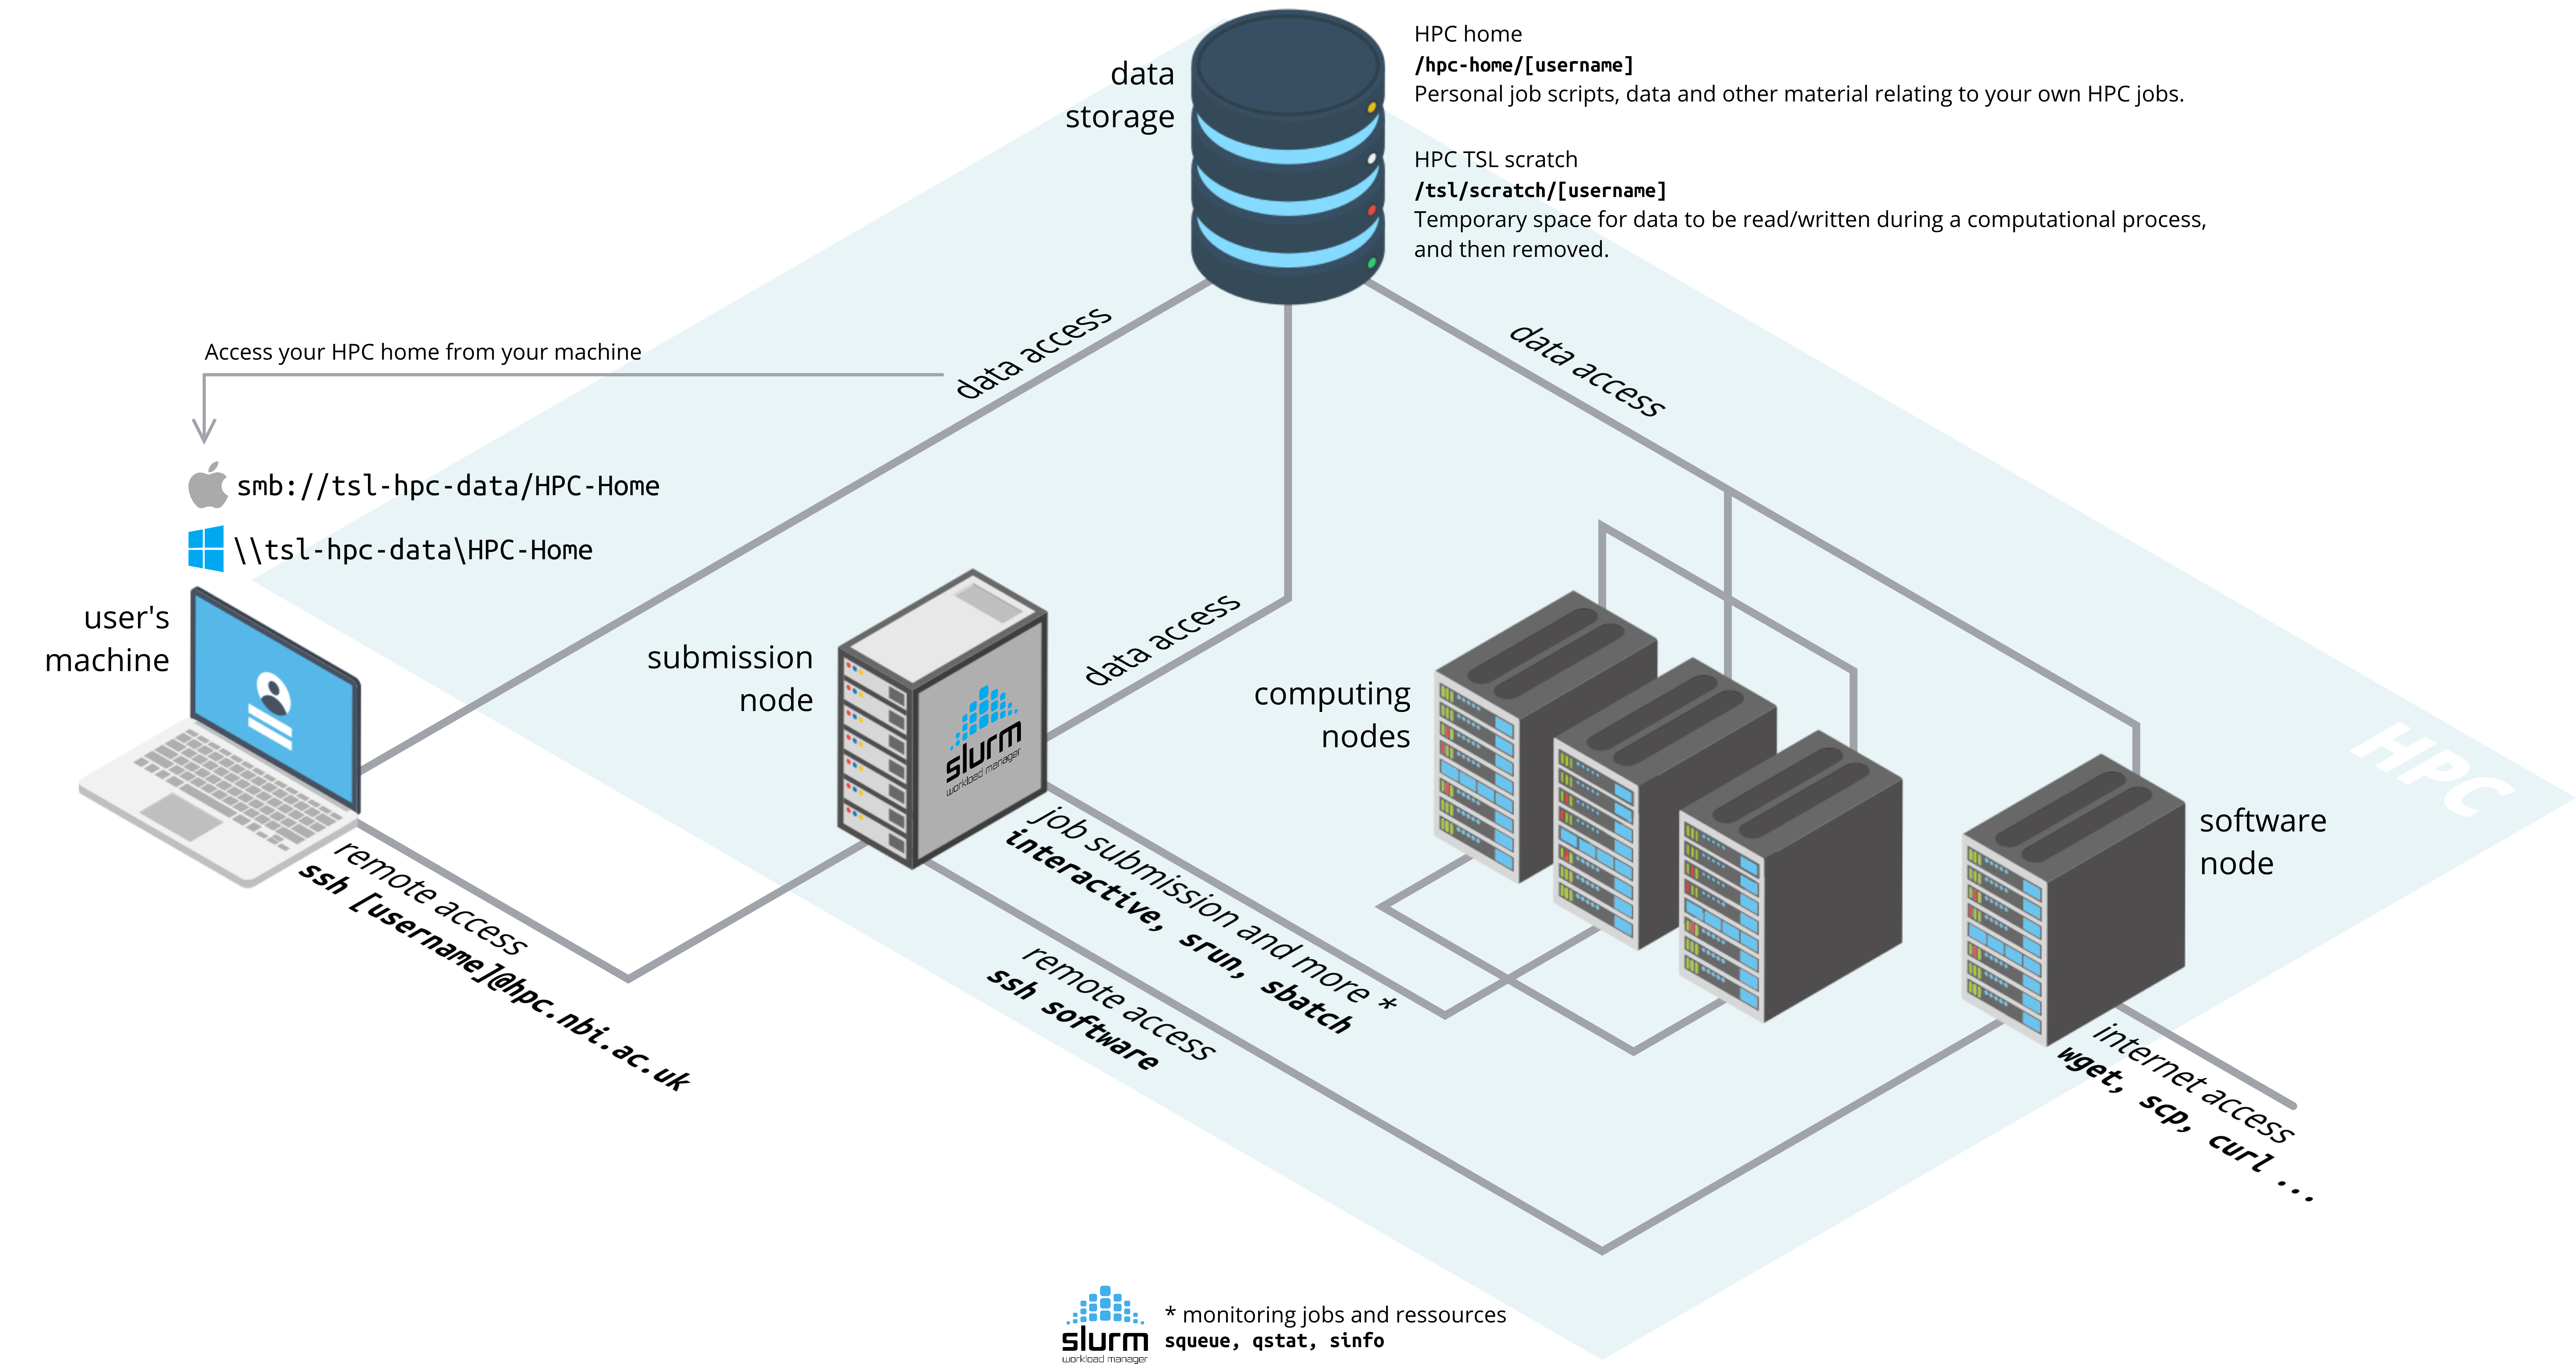
\includegraphics[keepaspectratio]{images/hpc-overview.png}}

The remote server is a
\href{https://en.wikipedia.org/wiki/Computer_cluster}{computer cluster}
used for high performance computing (HPC) for the Norwich BioScience
Institutes (NBI). You can log into the remote server using the command
\texttt{ssh}, your username and the address of the server
\texttt{hpc.nbi.ac.uk} (make sure to replace \texttt{{[}username{]}} by
your actual TSL username).

\begin{Shaded}
\begin{Highlighting}[]
\FunctionTok{ssh} \PreprocessorTok{[}\SpecialStringTok{username}\PreprocessorTok{]}\NormalTok{@hpc.nbi.ac.uk}
\end{Highlighting}
\end{Shaded}

You must then input your password.

\begin{figure}

\begin{minipage}{0.50\linewidth}

\begin{figure}[H]

{\centering \pandocbounded{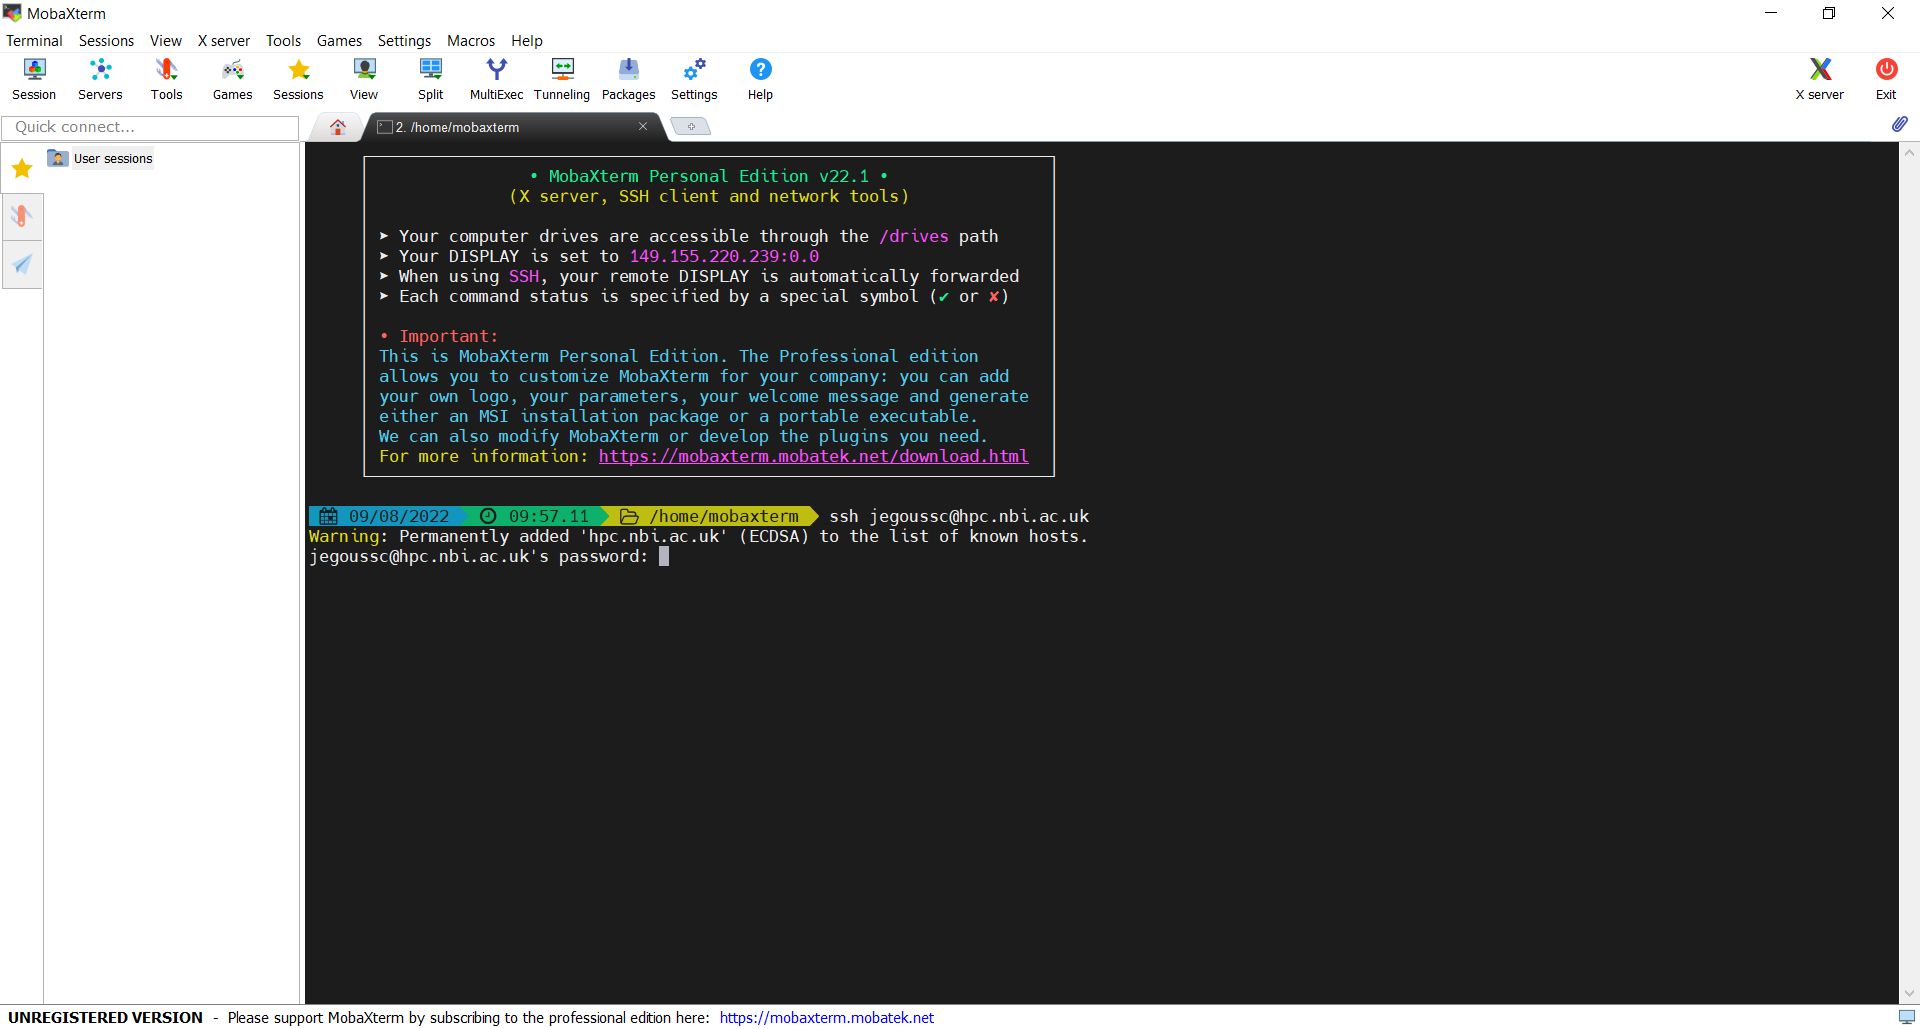
\includegraphics[keepaspectratio]{images/ssh-hpc-nbi.png}}

}

\subcaption{Windows}

\end{figure}%

\end{minipage}%
%
\begin{minipage}{0.50\linewidth}

\begin{figure}[H]

{\centering \pandocbounded{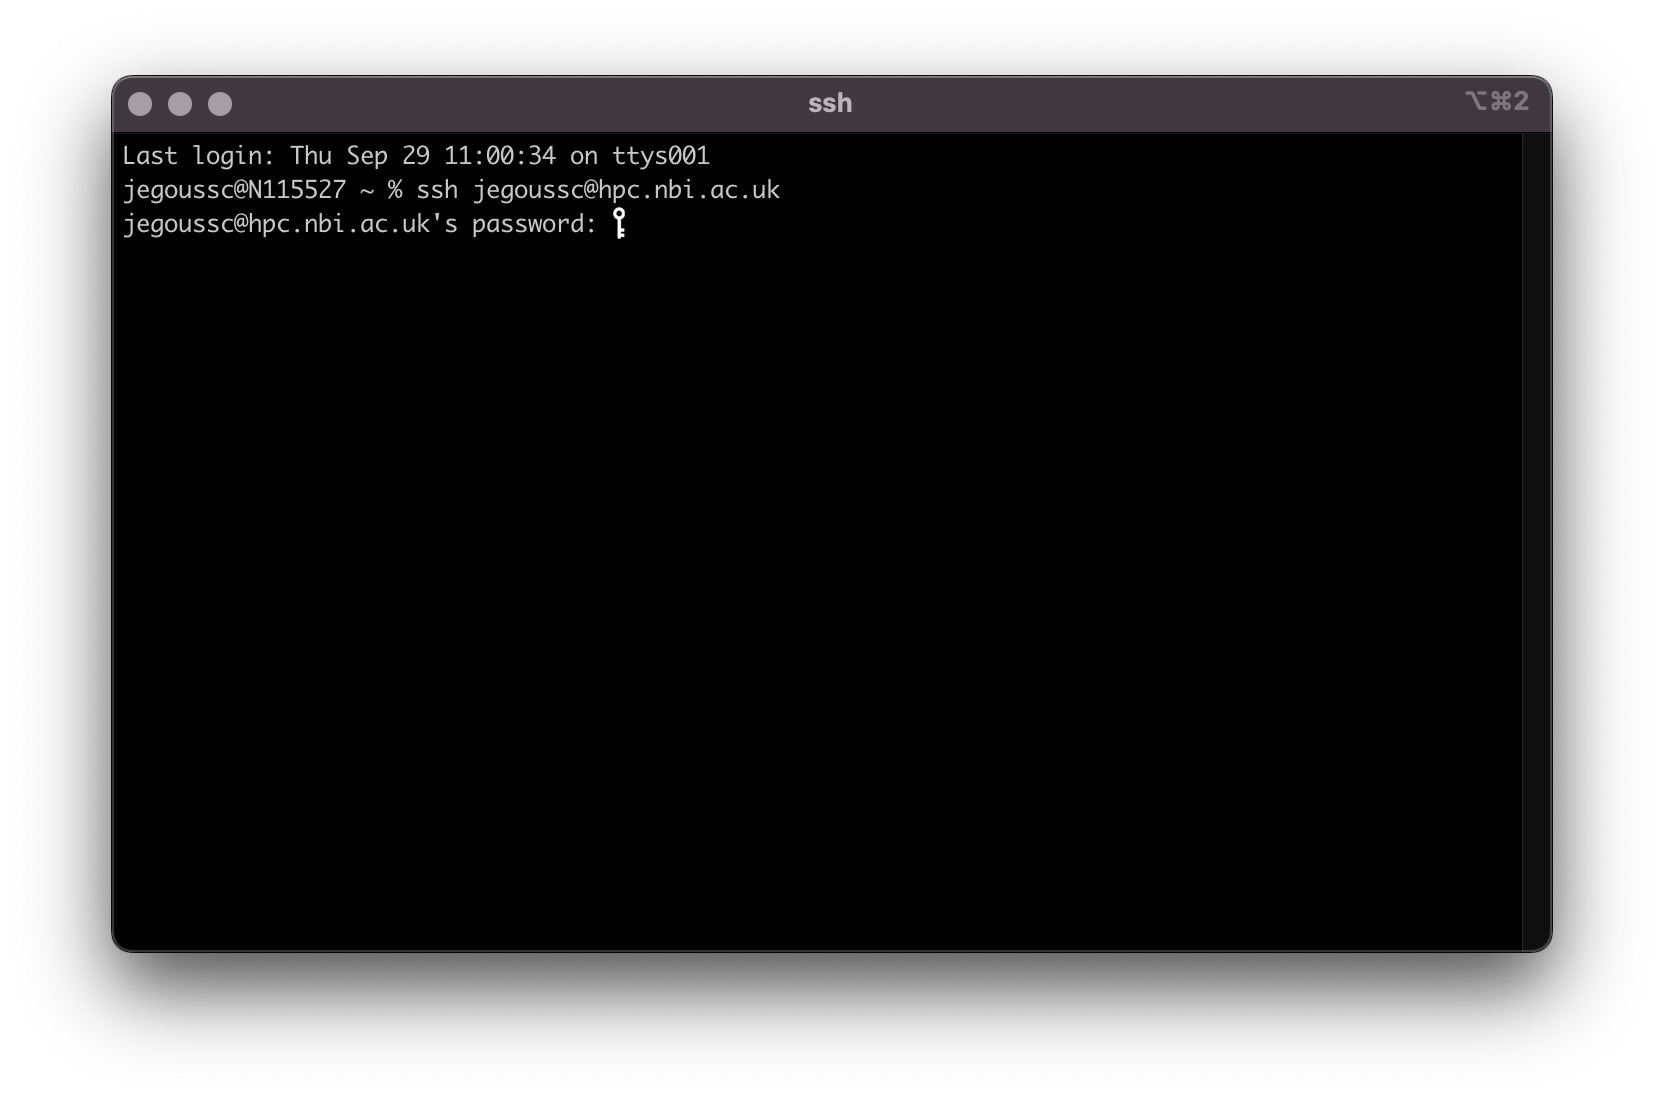
\includegraphics[keepaspectratio]{images/ssh-hpc-nbi-mac.png}}

}

\subcaption{MacOS}

\end{figure}%

\end{minipage}%

\end{figure}%

\begin{tcolorbox}[enhanced jigsaw, opacitybacktitle=0.6, colback=white, coltitle=black, opacityback=0, rightrule=.15mm, toptitle=1mm, toprule=.15mm, bottomtitle=1mm, colframe=quarto-callout-note-color-frame, arc=.35mm, titlerule=0mm, colbacktitle=quarto-callout-note-color!10!white, leftrule=.75mm, title=\textcolor{quarto-callout-note-color}{\faInfo}\hspace{0.5em}{Save your password for later}, breakable, bottomrule=.15mm, left=2mm]

MobaXterm will offer for you to save your password. It is up to you to
do so.

\begin{figure}[H]

{\centering 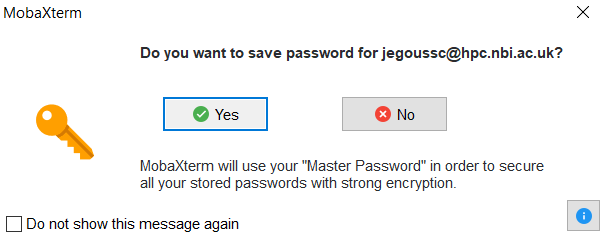
\includegraphics[width=5.20833in,height=\textheight,keepaspectratio]{images/password-save.png}

}

\caption{Windows}

\end{figure}%%
\begin{figure}[H]

{\centering 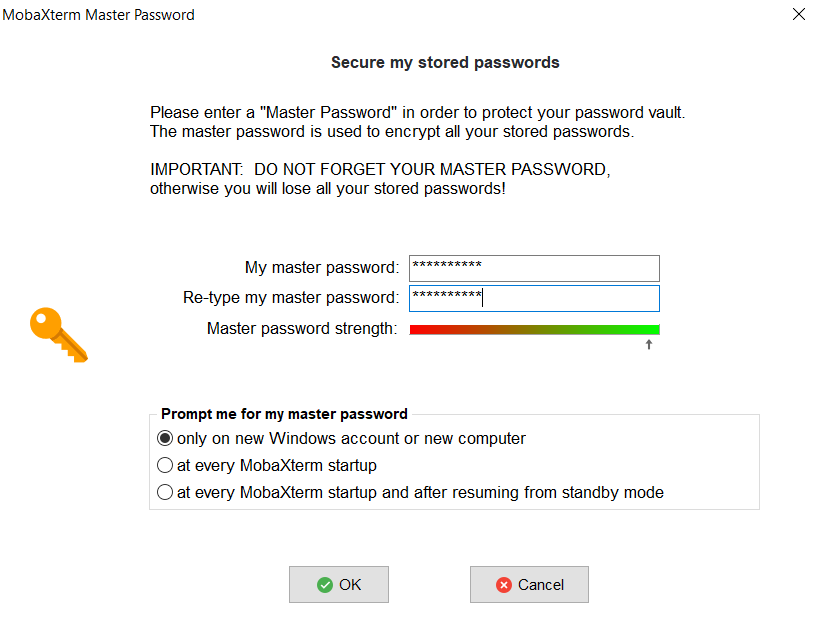
\includegraphics[width=5.20833in,height=\textheight,keepaspectratio]{images/master-password.png}

}

\caption{MacOS}

\end{figure}%

\end{tcolorbox}

After entering you password, you will be logged in the server and see
the welcome message as seen in the screen capture below:

\begin{figure}

\begin{minipage}{0.50\linewidth}

\begin{figure}[H]

{\centering \pandocbounded{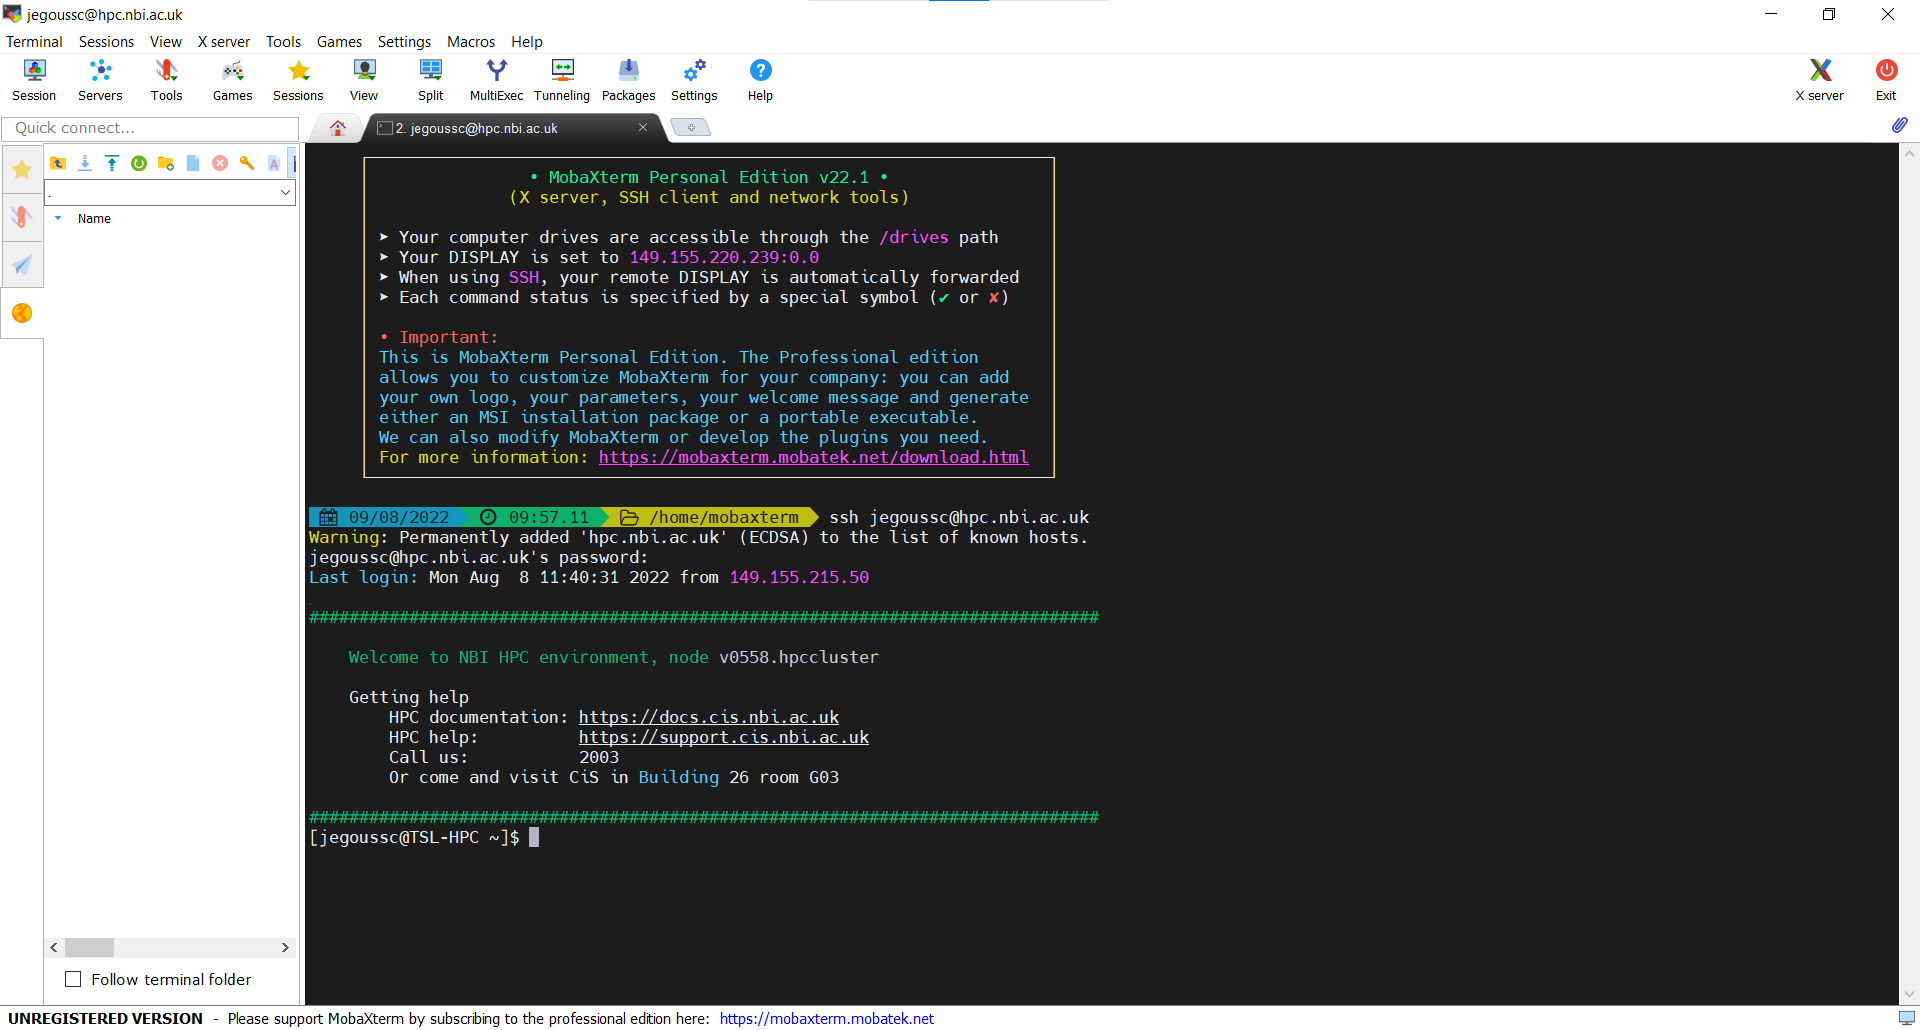
\includegraphics[keepaspectratio]{images/welcome-to-nbi-hpc.png}}

}

\subcaption{Windows}

\end{figure}%

\end{minipage}%
%
\begin{minipage}{0.50\linewidth}

\begin{figure}[H]

{\centering \pandocbounded{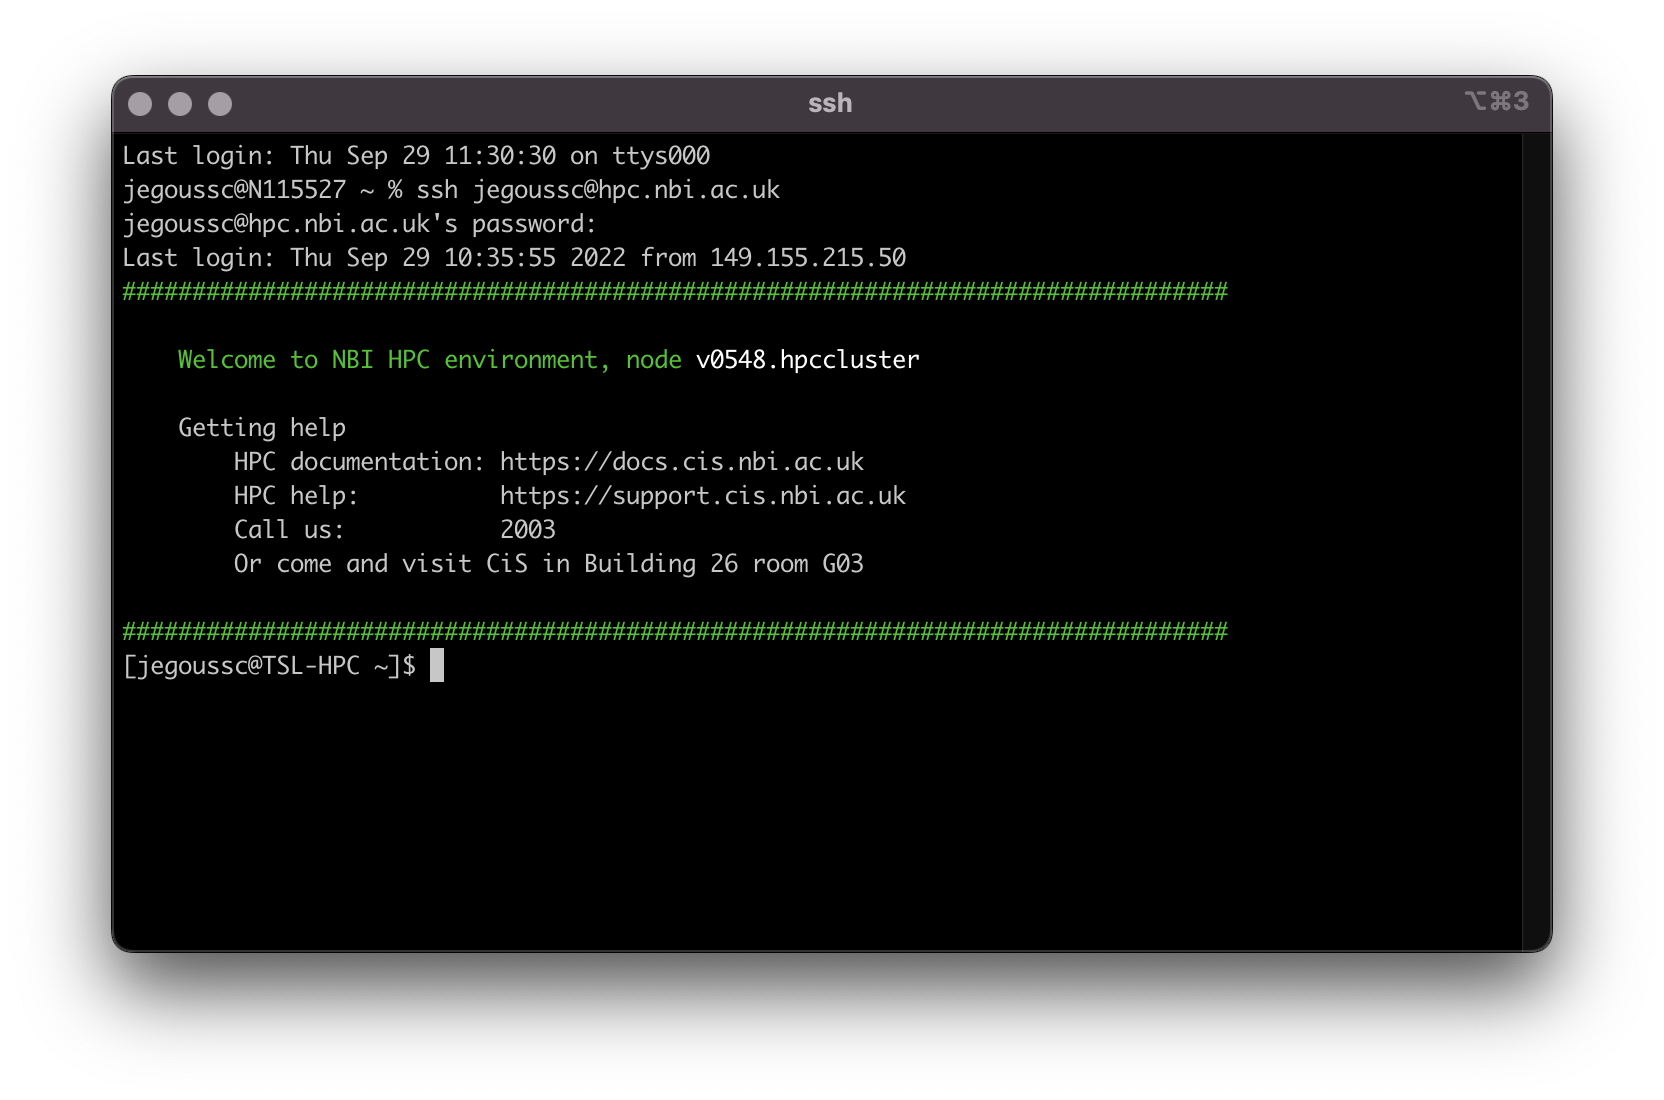
\includegraphics[keepaspectratio]{images/welcome-to-nbi-hpc-mac.png}}

}

\subcaption{MacOS}

\end{figure}%

\end{minipage}%

\end{figure}%

This welcome message provides a lot of information about the remote
server that you're logging into. We're not going to use most of this
information for our workshop, so you can clear your screen using the
\texttt{clear} command.

Type the word \texttt{clear} into the terminal and press the
\texttt{Enter} key.

This will scroll your screen down to give you a fresh screen and will
make it easier to read. You haven't lost any of the information on your
screen. If you scroll up, you can see everything that has been output to
your screen up until this point.

\begin{tcolorbox}[enhanced jigsaw, opacitybacktitle=0.6, colback=white, coltitle=black, opacityback=0, rightrule=.15mm, toptitle=1mm, toprule=.15mm, bottomtitle=1mm, colframe=quarto-callout-tip-color-frame, arc=.35mm, titlerule=0mm, colbacktitle=quarto-callout-tip-color!10!white, leftrule=.75mm, title=\textcolor{quarto-callout-tip-color}{\faLightbulb}\hspace{0.5em}{Tip}, breakable, bottomrule=.15mm, left=2mm]

Hot-key combinations are shortcuts for performing common commands. The
hot-key combination for clearing the console is \texttt{Ctrl+L}. Feel
free to try it and see for yourself.

\end{tcolorbox}

\section{Navigating your file system}\label{navigating-your-file-system}

The part of the operating system that manages files and directories is
called the \textbf{file system}. It organizes our data into files, which
hold information, and directories (also called ``folders''), which hold
files or other directories.

Several commands are frequently used to create, inspect, rename, and
delete files and directories.

\subsection{Prompt}\label{prompt}

The dollar sign is a \textbf{prompt}, which shows us that the shell is
waiting for input (other shell may use a different character as a prompt
and may add information before the prompt). When typing commands, either
from these lessons or from other sources, do not type the prompt, only
the commands that follow it.

\begin{Shaded}
\begin{Highlighting}[]
\ExtensionTok{$}
\end{Highlighting}
\end{Shaded}

\subsection{Print working directory}\label{print-working-directory}

Let's find out where we are by running a command called \texttt{pwd}
(which stands for ``\textbf{p}rint \textbf{w}orking
\textbf{d}irectory''). At any moment, our \textbf{current working
directory} is our current default directory, i.e., the directory that
the computer assumes we want to run commands in, unless we explicitly
specify something else. Here, the computer's response is
\texttt{/hpc-home/{[}username{]}}, which is the top level directory
within our server:

\begin{Shaded}
\begin{Highlighting}[]
\ExtensionTok{$}\NormalTok{ pwd}
\ExtensionTok{/hpc{-}home/[username]}
\end{Highlighting}
\end{Shaded}

\subsection{Listing}\label{listing}

Let's look at how our file system is organized. We can see what files
and subdirectories are in this directory by running \texttt{ls}, which
stands for ``listing'':

\begin{Shaded}
\begin{Highlighting}[]
\ExtensionTok{$}\NormalTok{ ls}
\end{Highlighting}
\end{Shaded}

\texttt{ls} prints the names of the files and directories in the current
directory in alphabetical order, arranged neatly into columns. We'll be
working within the \texttt{shell\_data} subdirectory, and creating new
subdirectories, throughout this workshop.

\subsection{Make new directory}\label{make-new-directory}

Let's make a new directory (folder) called \texttt{shell\_data} for
today's session using the command \texttt{mkdir} for
``\textbf{m}a\textbf{k}e \textbf{dir}ectory'':

\begin{Shaded}
\begin{Highlighting}[]
\ExtensionTok{$}\NormalTok{ mkdir shell\_data}
\end{Highlighting}
\end{Shaded}

Now let's see our new directory using the listing command \texttt{ls}:

\begin{Shaded}
\begin{Highlighting}[]
\ExtensionTok{$}\NormalTok{ ls}
\end{Highlighting}
\end{Shaded}

\subsection{Copy directory}\label{copy-directory}

Our home directory is empty. Let's copy a directory called
\texttt{shell\_data} from the home directory of user \texttt{jegoussc}
using the command \texttt{cp} for ``\textbf{c}o\textbf{p}y''. The flag
\texttt{-r} stands for ``recursive'' and specifies that we want to copy
the full content of the directory \texttt{shell\_data}:

\begin{Shaded}
\begin{Highlighting}[]
\ExtensionTok{$}\NormalTok{ cp }\AttributeTok{{-}r}\NormalTok{ /tsl/data/shell\_data/ /hpc{-}home/}\PreprocessorTok{[}\SpecialStringTok{username}\PreprocessorTok{]}\NormalTok{/}
\end{Highlighting}
\end{Shaded}

\subsection{Change directory}\label{change-directory}

The command to change locations in our file system is \texttt{cd},
followed by a directory name to change our working directory.
\texttt{cd} stands for ``\textbf{c}hange \textbf{d}irectory''.

\begin{Shaded}
\begin{Highlighting}[]
\ExtensionTok{$}\NormalTok{ cd shell\_data}
\end{Highlighting}
\end{Shaded}

We can also use the command \texttt{pwd} to print the current working
directory:

\begin{Shaded}
\begin{Highlighting}[]
\ExtensionTok{$}\NormalTok{ pwd}
\end{Highlighting}
\end{Shaded}

\subsection{Flags}\label{flags}

Earlier, we used the flag \texttt{-r} with the \texttt{cp} command.
Let's have a look at the content of the directory now. We can make the
\texttt{ls} output more comprehensible by using the \textbf{flag}
\texttt{-F}, which tells \texttt{ls} to add a trailing \texttt{/} to the
names of directories:

\begin{Shaded}
\begin{Highlighting}[]
\ExtensionTok{$}\NormalTok{ ls }\AttributeTok{{-}F}
\ExtensionTok{sra\_metadata/}\NormalTok{  untrimmed\_fastq/}
\end{Highlighting}
\end{Shaded}

Anything with a ``/'' after it is a directory. Things with a ``*'' after
them are programs. If there are no decorations, it's a file.

\subsection{Manuals}\label{manuals}

\texttt{ls} has lots of other options. To find out what they are, we can
type:

\begin{Shaded}
\begin{Highlighting}[]
\ExtensionTok{$}\NormalTok{ man ls}
\end{Highlighting}
\end{Shaded}

\texttt{man} (short for ``\textbf{man}ual'') displays detailed
documentation (also referred as man page or man file) for \texttt{bash}
commands. It is a powerful resource to explore \texttt{bash} commands,
understand their usage and flags. Some manual files are very long. You
can scroll through the file using your keyboard's down arrow or use the
\texttt{Space} key to go forward one page and the b key to go backwards
one page. When you are done reading, hit the key \texttt{q} to quit.

\begin{tcolorbox}[enhanced jigsaw, opacitybacktitle=0.6, colback=white, coltitle=black, opacityback=0, rightrule=.15mm, toptitle=1mm, toprule=.15mm, bottomtitle=1mm, colframe=quarto-callout-caution-color-frame, arc=.35mm, titlerule=0mm, colbacktitle=quarto-callout-caution-color!10!white, leftrule=.75mm, title={Exercise}, breakable, bottomrule=.15mm, left=2mm]

Use the \texttt{-l} option for the \texttt{ls} command to display more
information for each item in the directory. What is one piece of
additional information this long format gives you that you don't see
with the bare \texttt{ls} command?

\end{tcolorbox}

\begin{tcolorbox}[enhanced jigsaw, opacitybacktitle=0.6, colback=white, coltitle=black, opacityback=0, rightrule=.15mm, toptitle=1mm, toprule=.15mm, bottomtitle=1mm, colframe=quarto-callout-caution-color-frame, arc=.35mm, titlerule=0mm, colbacktitle=quarto-callout-caution-color!10!white, leftrule=.75mm, title={Solution}, breakable, bottomrule=.15mm, left=2mm]

\begin{verbatim}
$ ls -l
\end{verbatim}

\end{tcolorbox}

No one can possibly learn all of these arguments, that's what the manual
page is for. You can (and should) refer to the manual page or other help
files as needed.

Let's go into the \texttt{untrimmed\_fastq} directory and see what is in
there.

\begin{Shaded}
\begin{Highlighting}[]
\ExtensionTok{$}\NormalTok{ cd untrimmed\_fastq}
\ExtensionTok{$}\NormalTok{ ls }\AttributeTok{{-}F}
\ExtensionTok{SRR097977.fastq*}\NormalTok{  SRR098026.fastq}\PreprocessorTok{*}
\end{Highlighting}
\end{Shaded}

This directory contains two files with \texttt{.fastq} extensions. FASTQ
is a format for storing information about sequencing reads and their
quality. We will be learning more about FASTQ files in a later lesson.

\subsection{Tab Completion}\label{tab-completion}

Typing out file or directory names can waste a lot of time and it's easy
to make typing mistakes. Instead we can use tab complete as a shortcut.
When you start typing out the name of a directory or file, then hit the
Tab key, the shell will try to fill in the rest of the directory or file
name.

Return to your home directory:

\begin{Shaded}
\begin{Highlighting}[]
\ExtensionTok{$}\NormalTok{ cd}
\end{Highlighting}
\end{Shaded}

then enter (\texttt{\textless{}tab\textgreater{}} to hit the tabulation
key):

\begin{Shaded}
\begin{Highlighting}[]
\ExtensionTok{$}\NormalTok{ cd she}\OperatorTok{\textless{}}\NormalTok{tab}\OperatorTok{\textgreater{}}
\end{Highlighting}
\end{Shaded}

The shell will fill in the rest of the directory name for
\texttt{shell\_data} and auto-complete the command:

\begin{Shaded}
\begin{Highlighting}[]
\ExtensionTok{$}\NormalTok{ cd shell\_data}
\end{Highlighting}
\end{Shaded}

Now change directories to \texttt{untrimmed\_fastq} in
\texttt{shell\_data}

\begin{Shaded}
\begin{Highlighting}[]
\ExtensionTok{$}\NormalTok{ cd untrimmed\_fastq}
\end{Highlighting}
\end{Shaded}

Using tab complete can be very helpful. However, it will only
auto-complete a file or directory name if you've typed enough characters
to provide a unique identifier for the file or directory you are trying
to access.

For example, if we now try to list the files which names start with
\texttt{SR} by using tab complete:

\begin{Shaded}
\begin{Highlighting}[]
\ExtensionTok{$}\NormalTok{ ls SR}\OperatorTok{\textless{}}\NormalTok{tab}\OperatorTok{\textgreater{}}
\end{Highlighting}
\end{Shaded}

The shell auto-completes your command to \texttt{SRR09}, because all
file names in the directory begin with this prefix. When you hit Tab
again, the shell will list the possible choices.

\begin{Shaded}
\begin{Highlighting}[]
\ExtensionTok{$}\NormalTok{ ls SRR09}\OperatorTok{\textless{}}\NormalTok{tab}\OperatorTok{\textgreater{}\textless{}}\NormalTok{tab}\OperatorTok{\textgreater{}}
\ExtensionTok{SRR097977.fastq}\NormalTok{  SRR098026.fastq}
\end{Highlighting}
\end{Shaded}

Tab completion can also fill in the names of programs, which can be
useful if you remember the beginning of a program name.

\begin{Shaded}
\begin{Highlighting}[]
\ExtensionTok{$}\NormalTok{ pw}\OperatorTok{\textless{}}\NormalTok{tab}\OperatorTok{\textgreater{}\textless{}}\NormalTok{tab}\OperatorTok{\textgreater{}}
\ExtensionTok{pwck}\NormalTok{      pwconv    pwd       pwdx      pwunconv  pwmake  pwscore}
\end{Highlighting}
\end{Shaded}

Displays the name of every program that starts with \texttt{pw}.

\section{Summary}\label{summary}

We now know how to move around our file system using the command line.
This gives us an advantage over interacting with the file system through
a GUI as it allows us to work on a remote server, carry out the same set
of operations on a large number of files quickly, and opens up many
opportunities for using bioinformatic software that is only available in
command line versions.

In the next few episodes, we'll be expanding on these skills and seeing
how using the command line shell enables us to make our workflow more
efficient and reproducible.

\begin{tcolorbox}[enhanced jigsaw, opacitybacktitle=0.6, colback=white, coltitle=black, opacityback=0, rightrule=.15mm, toptitle=1mm, toprule=.15mm, bottomtitle=1mm, colframe=quarto-callout-important-color-frame, arc=.35mm, titlerule=0mm, colbacktitle=quarto-callout-important-color!10!white, leftrule=.75mm, title=\textcolor{quarto-callout-important-color}{\faExclamation}\hspace{0.5em}{Key points}, breakable, bottomrule=.15mm, left=2mm]

\begin{itemize}
\tightlist
\item
  The shell gives you the ability to work more efficiently by using
  keyboard commands rather than a GUI.
\item
  Useful commands for navigating your file system include: \texttt{ls},
  \texttt{pwd}, and \texttt{cd}.
\item
  Most commands take options (flags) which begin with a \texttt{-}.
\item
  Tab completion can reduce errors from mistyping and make work more
  efficient in the shell.
\end{itemize}

\end{tcolorbox}

\bookmarksetup{startatroot}

\chapter{Navigating Files and
Directories}\label{sec-navigating-files-and-directories}

\begin{tcolorbox}[enhanced jigsaw, opacitybacktitle=0.6, colback=white, coltitle=black, opacityback=0, rightrule=.15mm, toptitle=1mm, toprule=.15mm, bottomtitle=1mm, colframe=quarto-callout-note-color-frame, arc=.35mm, titlerule=0mm, colbacktitle=quarto-callout-note-color!10!white, leftrule=.75mm, title={⏳ Time}, breakable, bottomrule=.15mm, left=2mm]

\begin{itemize}
\tightlist
\item
  Teaching: 30 min
\item
  Exercises: 20 min
\end{itemize}

\end{tcolorbox}

\begin{tcolorbox}[enhanced jigsaw, opacitybacktitle=0.6, colback=white, coltitle=black, opacityback=0, rightrule=.15mm, toptitle=1mm, toprule=.15mm, bottomtitle=1mm, colframe=quarto-callout-important-color-frame, arc=.35mm, titlerule=0mm, colbacktitle=quarto-callout-important-color!10!white, leftrule=.75mm, title={🎯 Objectives}, breakable, bottomrule=.15mm, left=2mm]

\begin{itemize}
\tightlist
\item
  Use a single command to navigate multiple steps in your directory
  structure, including moving backwards (one level up).
\item
  Perform operations on files in directories outside your working
  directory.
\item
  Work with hidden directories and hidden files.
\item
  Inter-convert between absolute and relative paths.
\item
  Employ navigational shortcuts to move around your file system.
\end{itemize}

\end{tcolorbox}

\section{Moving around the file
system}\label{moving-around-the-file-system}

We've learned how to use \texttt{pwd} to find our current location
within our file system. We've also learned how to use \texttt{cd} to
change locations and \texttt{ls} to list the contents of a directory.
Now we're going to learn some additional commands for moving around
within our file system.

Use the commands we've learned so far to navigate to the
\texttt{shell\_data/untrimmed\_fastq} directory, if you're not already
there.

\begin{Shaded}
\begin{Highlighting}[]
\ExtensionTok{$}\NormalTok{ cd}
\ExtensionTok{$}\NormalTok{ cd shell\_data}
\ExtensionTok{$}\NormalTok{ cd untrimmed\_fastq}
\end{Highlighting}
\end{Shaded}

What if we want to move back up and out of this directory and to our top
level directory? Can we type \texttt{cd\ shell\_data}? Try it and see
what happens.

\begin{Shaded}
\begin{Highlighting}[]
\ExtensionTok{$}\NormalTok{ cd shell\_data}
\ExtensionTok{{-}bash:}\NormalTok{ cd: shell\_data: No such file or director}
\end{Highlighting}
\end{Shaded}

Your computer looked for a directory or file called \texttt{shell\_data}
within the directory you were already in. It didn't know you wanted to
look at a directory level above the one you were located in.

We have a special command to tell the computer to move us back or up one
directory level.

\begin{Shaded}
\begin{Highlighting}[]
\ExtensionTok{$}\NormalTok{ cd ..}
\end{Highlighting}
\end{Shaded}

Now we can use \texttt{pwd} to make sure that we are in the directory we
intended to navigate to, and \texttt{ls} to check that the contents of
the directory are correct.

\begin{Shaded}
\begin{Highlighting}[]
\ExtensionTok{$}\NormalTok{ pwd}
\ExtensionTok{/hpc{-}home/[username]/shell\_data}
\end{Highlighting}
\end{Shaded}

\begin{Shaded}
\begin{Highlighting}[]
\ExtensionTok{$}\NormalTok{ ls}
\ExtensionTok{sra\_metadata}\NormalTok{  untrimmed\_fastq}
\end{Highlighting}
\end{Shaded}

From this output, we can see that \texttt{..} did indeed take us back
one level in our file system.

You can chain these together like so:

\begin{Shaded}
\begin{Highlighting}[]
\ExtensionTok{$}\NormalTok{ ls ../../}
\end{Highlighting}
\end{Shaded}

prints the contents of \texttt{/hpc-home}.

\section{Hidden directories}\label{hidden-directories}

\begin{tcolorbox}[enhanced jigsaw, opacitybacktitle=0.6, colback=white, coltitle=black, opacityback=0, rightrule=.15mm, toptitle=1mm, toprule=.15mm, bottomtitle=1mm, colframe=quarto-callout-caution-color-frame, arc=.35mm, titlerule=0mm, colbacktitle=quarto-callout-caution-color!10!white, leftrule=.75mm, title={Exercise}, breakable, bottomrule=.15mm, left=2mm]

Find hidden directories.

First navigate to the \texttt{shell\_data} directory. There is a hidden
directory within this directory. Explore the options for \texttt{ls} to
find out how to see hidden directories. List the contents of the
directory and identify the name of the text file in that directory.

Hint: hidden files and folders in Unix start with \texttt{.}, for
example \texttt{.my\_hidden\_directory}

\end{tcolorbox}

\begin{tcolorbox}[enhanced jigsaw, opacitybacktitle=0.6, colback=white, coltitle=black, opacityback=0, rightrule=.15mm, toptitle=1mm, toprule=.15mm, bottomtitle=1mm, colframe=quarto-callout-caution-color-frame, arc=.35mm, titlerule=0mm, colbacktitle=quarto-callout-caution-color!10!white, leftrule=.75mm, title={Solution}, breakable, bottomrule=.15mm, left=2mm]

First use the \texttt{man} command to look at the options for
\texttt{ls}.

\begin{Shaded}
\begin{Highlighting}[]
\ExtensionTok{$}\NormalTok{ man ls}
\end{Highlighting}
\end{Shaded}

The \texttt{-a} option is short for \texttt{all} and says that it causes
\texttt{ls} to ``not ignore entries starting with .'' This is the option
we want.

\begin{Shaded}
\begin{Highlighting}[]
\ExtensionTok{$}\NormalTok{ ls }\AttributeTok{{-}a}
\BuiltInTok{.}\NormalTok{  ..  .hidden  sra\_metadata  untrimmed\_fastq}
\end{Highlighting}
\end{Shaded}

The name of the hidden directory is \texttt{.hidden}. We can navigate to
that directory using \texttt{cd}.

\begin{Shaded}
\begin{Highlighting}[]
\BuiltInTok{cd}\NormalTok{ .hidden}
\end{Highlighting}
\end{Shaded}

And then list the contents of the directory using \texttt{ls}.

\begin{verbatim}
$ ls
youfoundit.txt
\end{verbatim}

The name of the text file is \texttt{youfoundit.txt}.

\end{tcolorbox}

In most commands the flags can be combined together in no particular
order to obtain the desired results/output.

\begin{Shaded}
\begin{Highlighting}[]
\ExtensionTok{$}\NormalTok{ ls }\AttributeTok{{-}Fa}
\ExtensionTok{$}\NormalTok{ ls }\AttributeTok{{-}laF}
\end{Highlighting}
\end{Shaded}

\section{Examining the contents of other
directories}\label{examining-the-contents-of-other-directories}

By default, the \texttt{ls} commands lists the contents of the working
directory (i.e.~the directory you are in). You can always find the
directory you are in using the \texttt{pwd} command. However, you can
also give \texttt{ls} the names of other directories to view. Navigate
to your home directory if you are not already there.

\begin{Shaded}
\begin{Highlighting}[]
\ExtensionTok{$}\NormalTok{ cd}
\end{Highlighting}
\end{Shaded}

Then enter the command:

\begin{Shaded}
\begin{Highlighting}[]
\ExtensionTok{$}\NormalTok{ ls shell\_data}
\ExtensionTok{sra\_metadata}\NormalTok{  untrimmed\_fastq}
\end{Highlighting}
\end{Shaded}

This will list the contents of the \texttt{shell\_data} directory
without you needing to navigate there. The \texttt{cd} command works in
a similar way.

Try entering:

\begin{Shaded}
\begin{Highlighting}[]
\ExtensionTok{$}\NormalTok{ cd}
\ExtensionTok{$}\NormalTok{ cd shell\_data/untrimmed\_fastq}
\end{Highlighting}
\end{Shaded}

This will take you to the \texttt{untrimmed\_fastq} directory without
having to go through the intermediate directory.

\begin{tcolorbox}[enhanced jigsaw, opacitybacktitle=0.6, colback=white, coltitle=black, opacityback=0, rightrule=.15mm, toptitle=1mm, toprule=.15mm, bottomtitle=1mm, colframe=quarto-callout-caution-color-frame, arc=.35mm, titlerule=0mm, colbacktitle=quarto-callout-caution-color!10!white, leftrule=.75mm, title={Exercise}, breakable, bottomrule=.15mm, left=2mm]

Navigate to your home directory. From there, list the contents of the
\texttt{untrimmed\_fastq} directory.

\end{tcolorbox}

\begin{tcolorbox}[enhanced jigsaw, opacitybacktitle=0.6, colback=white, coltitle=black, opacityback=0, rightrule=.15mm, toptitle=1mm, toprule=.15mm, bottomtitle=1mm, colframe=quarto-callout-caution-color-frame, arc=.35mm, titlerule=0mm, colbacktitle=quarto-callout-caution-color!10!white, leftrule=.75mm, title={Solution}, breakable, bottomrule=.15mm, left=2mm]

\begin{Shaded}
\begin{Highlighting}[]
\ExtensionTok{$}\NormalTok{ cd}
\ExtensionTok{$}\NormalTok{ ls shell\_data/untrimmed\_fastq/}
\ExtensionTok{SRR097977.fastq}\NormalTok{  SRR098026.fastq }
\end{Highlighting}
\end{Shaded}

\end{tcolorbox}

\section{Full vs.~Relative Paths}\label{full-vs.-relative-paths}

The \texttt{cd} command takes an argument which is a directory name.
Directories can be specified using either a \emph{relative} path or a
full \emph{absolute} path. The directories on the computer are arranged
into a hierarchy. The full path tells you where a directory is in that
hierarchy. Navigate to the home directory, then enter the \texttt{pwd}
command.

\begin{Shaded}
\begin{Highlighting}[]
\ExtensionTok{$}\NormalTok{ cd  }
\ExtensionTok{$}\NormalTok{ pwd  }
\ExtensionTok{/hpc{-}home/[username]}
\end{Highlighting}
\end{Shaded}

This is the full name of your home directory. This tells you that you
are in a directory called \texttt{{[}username{]}}, which sits inside a
directory called \texttt{hpc-home} which sits inside the very top
directory in the hierarchy. The very top of the hierarchy is a directory
called \texttt{/} which is usually referred to as the \emph{root
directory}. So, to summarize: \texttt{{[}username{]}} is a directory in
\texttt{hpc-home} which is a directory in \texttt{/}. More on
\texttt{root} and \texttt{home} in the next section.

Now enter the following command:

\begin{Shaded}
\begin{Highlighting}[]
\ExtensionTok{$}\NormalTok{ cd /home/}\PreprocessorTok{[}\SpecialStringTok{username}\PreprocessorTok{]}\NormalTok{/shell\_data/.hidden}
\end{Highlighting}
\end{Shaded}

This jumps forward multiple levels to the \texttt{.hidden} directory.
Now go back to the home directory.

\begin{Shaded}
\begin{Highlighting}[]
\ExtensionTok{$}\NormalTok{ cd}
\end{Highlighting}
\end{Shaded}

You can also navigate to the \texttt{.hidden} directory using:

\begin{Shaded}
\begin{Highlighting}[]
\ExtensionTok{$}\NormalTok{ cd shell\_data/.hidden}
\end{Highlighting}
\end{Shaded}

These two commands have the same effect, they both take us to the
\texttt{.hidden} directory. The first uses the absolute path, giving the
full address from the home directory. The second uses a relative path,
giving only the address from the working directory. A full path always
starts with a \texttt{/}. A relative path does not.

A relative path is like getting directions from someone on the street.
They tell you to ``go right at the stop sign, and then turn left on Main
Street''. That works great if you're standing there together, but not so
well if you're trying to tell someone how to get there from another
country. A full path is like GPS coordinates. It tells you exactly where
something is no matter where you are right now.

You can usually use either a full path or a relative path depending on
what is most convenient. If we are in the home directory, it is more
convenient to enter the full path. If we are in the working directory,
it is more convenient to enter the relative path since it involves less
typing.

Over time, it will become easier for you to keep a mental note of the
structure of the directories that you are using and how to quickly
navigate among them.

\subsection{Navigational Shortcuts}\label{navigational-shortcuts}

The root directory is the highest level directory in your file system
and contains files that are important for your computer to perform its
daily work. While you will be using the root (\texttt{/}) at the
beginning of your absolute paths, it is important that you avoid working
with data in these higher-level directories, as your commands can
permanently alter files that the operating system needs to function. In
many cases, trying to run commands in \texttt{root} directories will
require special permissions which are not discussed here, so it's best
to avoid them and work within your home directory. Dealing with the
\texttt{home} directory is very common. The tilde character,
\texttt{\textasciitilde{}}, is a shortcut for your home directory. In
our case, the \texttt{root} directory is \textbf{two} levels above our
\texttt{home} directory, so \texttt{cd} or
\texttt{cd\ \textasciitilde{}} will take you to \texttt{/home/dcuser}
and \texttt{cd\ /} will take you to \texttt{/}. Navigate to the
\texttt{shell\_data} directory:

\begin{Shaded}
\begin{Highlighting}[]
\ExtensionTok{$}\NormalTok{ cd}
\ExtensionTok{$}\NormalTok{ cd shell\_data}
\end{Highlighting}
\end{Shaded}

Then enter the command:

\begin{Shaded}
\begin{Highlighting}[]
\ExtensionTok{$}\NormalTok{ ls \textasciitilde{}}
\end{Highlighting}
\end{Shaded}

This prints the contents of your home directory, without you needing to
type the full path.

The commands \texttt{cd}, and \texttt{cd\ \textasciitilde{}} are very
useful for quickly navigating back to your home directory. We will be
using the \texttt{\textasciitilde{}} character in later lessons to
specify our home directory.

\section{Summary}\label{summary-1}

\begin{tcolorbox}[enhanced jigsaw, opacitybacktitle=0.6, colback=white, coltitle=black, opacityback=0, rightrule=.15mm, toptitle=1mm, toprule=.15mm, bottomtitle=1mm, colframe=quarto-callout-important-color-frame, arc=.35mm, titlerule=0mm, colbacktitle=quarto-callout-important-color!10!white, leftrule=.75mm, title=\textcolor{quarto-callout-important-color}{\faExclamation}\hspace{0.5em}{Key points}, breakable, bottomrule=.15mm, left=2mm]

\begin{itemize}
\tightlist
\item
  The \texttt{/}, \texttt{\textasciitilde{}}, and \texttt{..} characters
  represent important navigational shortcuts.
\item
  Hidden files and directories start with \texttt{.} and can be viewed
  using \texttt{ls\ -a}.
\item
  Relative paths specify a location starting from the current location,
  while absolute paths specify a location from the root of the file
  system.
\end{itemize}

\end{tcolorbox}

\bookmarksetup{startatroot}

\chapter{Working with Files and
Directories}\label{sec-working-with-files-and-directories}

\begin{tcolorbox}[enhanced jigsaw, opacitybacktitle=0.6, colback=white, coltitle=black, opacityback=0, rightrule=.15mm, toptitle=1mm, toprule=.15mm, bottomtitle=1mm, colframe=quarto-callout-note-color-frame, arc=.35mm, titlerule=0mm, colbacktitle=quarto-callout-note-color!10!white, leftrule=.75mm, title={⏳ Time}, breakable, bottomrule=.15mm, left=2mm]

\begin{itemize}
\tightlist
\item
  Teaching: 30 min
\item
  Exercises: 15 min
\end{itemize}

\end{tcolorbox}

\begin{tcolorbox}[enhanced jigsaw, opacitybacktitle=0.6, colback=white, coltitle=black, opacityback=0, rightrule=.15mm, toptitle=1mm, toprule=.15mm, bottomtitle=1mm, colframe=quarto-callout-tip-color-frame, arc=.35mm, titlerule=0mm, colbacktitle=quarto-callout-tip-color!10!white, leftrule=.75mm, title={🤔 Questions}, breakable, bottomrule=.15mm, left=2mm]

\begin{itemize}
\tightlist
\item
  How can I view and search file contents?
\item
  How can I create, copy and delete files and directories?
\item
  How can I control who has permission to modify a file?
\item
  How can I repeat recently used commands?
\end{itemize}

\end{tcolorbox}

\begin{tcolorbox}[enhanced jigsaw, opacitybacktitle=0.6, colback=white, coltitle=black, opacityback=0, rightrule=.15mm, toptitle=1mm, toprule=.15mm, bottomtitle=1mm, colframe=quarto-callout-important-color-frame, arc=.35mm, titlerule=0mm, colbacktitle=quarto-callout-important-color!10!white, leftrule=.75mm, title={🎯 Objectives}, breakable, bottomrule=.15mm, left=2mm]

\begin{itemize}
\tightlist
\item
  View, search within, copy, move, and rename files. Create new
  directories.
\item
  Use wildcards (\texttt{*}) to perform operations on multiple files.
\item
  Make a file read only.
\item
  Use the \texttt{history} command to view and repeat recently used
  commands.
\end{itemize}

\end{tcolorbox}

\section{Working with Files}\label{working-with-files}

\subsection{Our data set of FASTQ
files}\label{our-data-set-of-fastq-files}

Now that we know how to navigate around our directory structure, let's
start working with our sequencing files. We did a sequencing experiment
and have two results files, which are stored in our
\texttt{untrimmed\_fastq} directory.

\subsection{Wildcards}\label{wildcards}

Navigate to your \texttt{untrimmed\_fastq} directory:

\begin{Shaded}
\begin{Highlighting}[]
\ExtensionTok{$}\NormalTok{ cd \textasciitilde{}/shell\_data/untrimmed\_fastq}
\end{Highlighting}
\end{Shaded}

We are interested in looking at the FASTQ files in this directory. We
can list all files with the .fastq extension using the command:

\begin{Shaded}
\begin{Highlighting}[]
\ExtensionTok{$}\NormalTok{ ls }\PreprocessorTok{*}\NormalTok{.fastq}
\ExtensionTok{SRR097977.fastq}\NormalTok{  SRR098026.fastq}
\end{Highlighting}
\end{Shaded}

The \texttt{*} character is a special type of character called a
wildcard, which can be used to represent any number of any type of
character. Thus, \texttt{*.fastq} matches every file that ends with
\texttt{.fastq}.

This command:

\begin{Shaded}
\begin{Highlighting}[]
\ExtensionTok{$}\NormalTok{ ls }\PreprocessorTok{*}\NormalTok{977.fastq}
\ExtensionTok{SRR097977.fastq}
\end{Highlighting}
\end{Shaded}

lists only the file that ends with \texttt{977.fastq}.

This command:

\begin{Shaded}
\begin{Highlighting}[]
\ExtensionTok{$}\NormalTok{ ls /usr/bin/}\PreprocessorTok{*}\NormalTok{.sh}
\ExtensionTok{/usr/bin/gettext.sh}\NormalTok{   /usr/bin/lprsetup.sh          /usr/bin/unix{-}lpr.sh}
\ExtensionTok{/usr/bin/lesspipe.sh}\NormalTok{  /usr/bin/setup{-}nsssysinit.sh}
\end{Highlighting}
\end{Shaded}

Lists every file in \texttt{/usr/bin} that ends in the characters
\texttt{.sh}. Note that the output displays \textbf{full} paths to
files, since each result starts with \texttt{/}.

\begin{tcolorbox}[enhanced jigsaw, opacitybacktitle=0.6, colback=white, coltitle=black, opacityback=0, rightrule=.15mm, toptitle=1mm, toprule=.15mm, bottomtitle=1mm, colframe=quarto-callout-caution-color-frame, arc=.35mm, titlerule=0mm, colbacktitle=quarto-callout-caution-color!10!white, leftrule=.75mm, title={Exercise}, breakable, bottomrule=.15mm, left=2mm]

Do each of the following tasks from your current directory using a
single \texttt{ls} command for each:

\begin{enumerate}
\def\labelenumi{\arabic{enumi}.}
\tightlist
\item
  List all of the files in \texttt{/usr/bin} that start with the letter
  `c'.
\item
  List all of the files in \texttt{/usr/bin} that contain the letter
  `a'.
\item
  List all of the files in \texttt{/usr/bin} that end with the letter
  `o'.
\end{enumerate}

Bonus: List all of the files in \texttt{/usr/bin} that contain the
letter `a' or the letter `c'.

Hint: The bonus question requires a Unix wildcard that we haven't talked
about yet. Try searching the internet for information about Unix
wildcards to find what you need to solve the bonus problem.

\end{tcolorbox}

\begin{tcolorbox}[enhanced jigsaw, opacitybacktitle=0.6, colback=white, coltitle=black, opacityback=0, rightrule=.15mm, toptitle=1mm, toprule=.15mm, bottomtitle=1mm, colframe=quarto-callout-caution-color-frame, arc=.35mm, titlerule=0mm, colbacktitle=quarto-callout-caution-color!10!white, leftrule=.75mm, title={Solution}, breakable, bottomrule=.15mm, left=2mm]

\begin{Shaded}
\begin{Highlighting}[]
\ExtensionTok{$}\NormalTok{ ls /usr/bin/c}\PreprocessorTok{*}
\ExtensionTok{$}\NormalTok{ ls /usr/bin/}\PreprocessorTok{*}\NormalTok{a}\PreprocessorTok{*}
\ExtensionTok{$}\NormalTok{ ls /usr/bin/}\PreprocessorTok{*}\NormalTok{o}

\CommentTok{\# Bonus}
\ExtensionTok{$}\NormalTok{ ls /usr/bin/}\PreprocessorTok{*[}\SpecialStringTok{ac}\PreprocessorTok{]*}
\end{Highlighting}
\end{Shaded}

\end{tcolorbox}

\section{Command History}\label{command-history}

If you want to repeat a command that you've run recently, you can access
previous commands using the up arrow on your keyboard to go back to the
most recent command. Likewise, the down arrow takes you forward in the
command history.

A few more useful shortcuts:

\begin{itemize}
\item
  \texttt{Ctrl} + \texttt{C} will cancel the command you are writing,
  and give you a fresh prompt.
\item
  \texttt{Ctrl} + \texttt{R} will do a reverse-search through your
  command history. This is very useful.
\item
  \texttt{Ctrl} + \texttt{L} or the \texttt{clear} command will clear
  your screen.
\end{itemize}

You can also review your recent commands with the \texttt{history}
command, by entering:

\begin{Shaded}
\begin{Highlighting}[]
\ExtensionTok{$}\NormalTok{ history}
\end{Highlighting}
\end{Shaded}

to see a numbered list of recent commands. You can reuse one of these
commands directly by referring to the number of that command.

For example, if your history looked like this:

\begin{Shaded}
\begin{Highlighting}[]
\ExtensionTok{259}\NormalTok{  ls }\PreprocessorTok{*}
\ExtensionTok{260}\NormalTok{  ls /usr/bin/}\PreprocessorTok{*}\NormalTok{.sh}
\ExtensionTok{261}\NormalTok{  ls }\PreprocessorTok{*}\NormalTok{R1}\PreprocessorTok{*}\NormalTok{fastq}
\end{Highlighting}
\end{Shaded}

then you could repeat command \#260 by entering:

\begin{Shaded}
\begin{Highlighting}[]
\ExtensionTok{$}\NormalTok{ !260}
\end{Highlighting}
\end{Shaded}

Type \texttt{!} (exclamation point) and then the number of the command
from your history. You will be glad you learned this when you need to
re-run very complicated commands. For more information on advanced usage
of \texttt{history}, read section 9.3 of
\href{https://www.gnu.org/software/bash/manual/html_node/index.html}{Bash
manual}.

\begin{tcolorbox}[enhanced jigsaw, opacitybacktitle=0.6, colback=white, coltitle=black, opacityback=0, rightrule=.15mm, toptitle=1mm, toprule=.15mm, bottomtitle=1mm, colframe=quarto-callout-caution-color-frame, arc=.35mm, titlerule=0mm, colbacktitle=quarto-callout-caution-color!10!white, leftrule=.75mm, title={Exercise}, breakable, bottomrule=.15mm, left=2mm]

Find the line number in your history for the command that listed all the
.sh files in \texttt{/usr/bin}. Rerun that command.

\end{tcolorbox}

\begin{tcolorbox}[enhanced jigsaw, opacitybacktitle=0.6, colback=white, coltitle=black, opacityback=0, rightrule=.15mm, toptitle=1mm, toprule=.15mm, bottomtitle=1mm, colframe=quarto-callout-caution-color-frame, arc=.35mm, titlerule=0mm, colbacktitle=quarto-callout-caution-color!10!white, leftrule=.75mm, title={Solution}, breakable, bottomrule=.15mm, left=2mm]

First type \texttt{history}. Then use \texttt{!} followed by the line
number to rerun that command.

\end{tcolorbox}

\section{Examining Files}\label{examining-files}

We now know how to switch directories, run programs, and look at the
contents of directories, but how do we look at the contents of files?

One way to examine a file is to print out all of the contents using the
program \texttt{cat}, for ``con\textbf{cat}enate''.

Enter the following command from within the \texttt{untrimmed\_fastq}
directory:

\begin{Shaded}
\begin{Highlighting}[]
\ExtensionTok{$}\NormalTok{ cat SRR098026.fastq}
\end{Highlighting}
\end{Shaded}

This will print out all of the contents of the \texttt{SRR098026.fastq}
to the screen.

\begin{tcolorbox}[enhanced jigsaw, opacitybacktitle=0.6, colback=white, coltitle=black, opacityback=0, rightrule=.15mm, toptitle=1mm, toprule=.15mm, bottomtitle=1mm, colframe=quarto-callout-caution-color-frame, arc=.35mm, titlerule=0mm, colbacktitle=quarto-callout-caution-color!10!white, leftrule=.75mm, title={Exercise}, breakable, bottomrule=.15mm, left=2mm]

\begin{enumerate}
\def\labelenumi{\arabic{enumi}.}
\tightlist
\item
  Print out the contents of the
  \texttt{\textasciitilde{}/shell\_data/untrimmed\_fastq/SRR097977.fastq}
  file. What is the last line of the file?
\item
  From your home directory, and without changing directories, use one
  short command to print the contents of all of the files in the
  \texttt{\textasciitilde{}/shell\_data/untrimmed\_fastq} directory.
\end{enumerate}

\end{tcolorbox}

\begin{tcolorbox}[enhanced jigsaw, opacitybacktitle=0.6, colback=white, coltitle=black, opacityback=0, rightrule=.15mm, toptitle=1mm, toprule=.15mm, bottomtitle=1mm, colframe=quarto-callout-caution-color-frame, arc=.35mm, titlerule=0mm, colbacktitle=quarto-callout-caution-color!10!white, leftrule=.75mm, title={Solution}, breakable, bottomrule=.15mm, left=2mm]

\begin{enumerate}
\def\labelenumi{\arabic{enumi}.}
\item
  The last line of the file is
  \texttt{C:CCC::CCCCCCCC\textless{}8?6A:C28C\textless{}608\textquotesingle{}\&\&\&,\textquotesingle{}\$}.
\item
  \texttt{cat\ \textasciitilde{}/shell\_data/untrimmed\_fastq/*}
\end{enumerate}

\end{tcolorbox}

\texttt{cat} is a terrific program, but when the file is really big, it
can be annoying to use. The program, \texttt{less}, is useful for this
case. \texttt{less} opens the file as read only, and lets you navigate
through it. The navigation commands are identical to the \texttt{man}
program.

Enter the following command:

\begin{Shaded}
\begin{Highlighting}[]
\ExtensionTok{$}\NormalTok{ less SRR097977.fastq}
\end{Highlighting}
\end{Shaded}

Some navigation commands in \texttt{less}:

\begin{longtable}[]{@{}ll@{}}
\toprule\noalign{}
key & action \\
\midrule\noalign{}
\endhead
\bottomrule\noalign{}
\endlastfoot
Space & to go forward \\
b & to go backward \\
g & to go to the beginning \\
G & to go to the end \\
q & to quit \\
\end{longtable}

\texttt{less} also gives you a way of searching through files. Use the
``/'' key to begin a search. Enter the word you would like to search for
and press \texttt{enter}. The screen will jump to the next location
where that word is found.

\begin{tcolorbox}[enhanced jigsaw, opacitybacktitle=0.6, colback=white, coltitle=black, opacityback=0, rightrule=.15mm, toptitle=1mm, toprule=.15mm, bottomtitle=1mm, colframe=quarto-callout-tip-color-frame, arc=.35mm, titlerule=0mm, colbacktitle=quarto-callout-tip-color!10!white, leftrule=.75mm, title=\textcolor{quarto-callout-tip-color}{\faLightbulb}\hspace{0.5em}{Shortcut}, breakable, bottomrule=.15mm, left=2mm]

\textbf{Shortcut:} If you hit ``/'' then ``enter'', \texttt{less} will
repeat the previous search. \texttt{less} searches from the current
location and works its way forward. Scroll up a couple lines on your
terminal to verify you are at the beginning of the file. Note, if you
are at the end of the file and search for the sequence ``CAA'',
\texttt{less} will not find it. You either need to go to the beginning
of the file (by typing \texttt{g}) and search again using \texttt{/} or
you can use \texttt{?} to search backwards in the same way you used
\texttt{/} previously.

For instance, let's search forward for the sequence \texttt{TTTTT} in
our file. You can see that we go right to that sequence, what it looks
like, and where it is in the file. If you continue to type \texttt{/}
and hit return, you will move forward to the next instance of this
sequence motif. If you instead type \texttt{?} and hit return, you will
search backwards and move up the file to previous examples of this
motif.

\end{tcolorbox}

\begin{tcolorbox}[enhanced jigsaw, opacitybacktitle=0.6, colback=white, coltitle=black, opacityback=0, rightrule=.15mm, toptitle=1mm, toprule=.15mm, bottomtitle=1mm, colframe=quarto-callout-caution-color-frame, arc=.35mm, titlerule=0mm, colbacktitle=quarto-callout-caution-color!10!white, leftrule=.75mm, title={Exercise}, breakable, bottomrule=.15mm, left=2mm]

What are the next three nucleotides (characters) after the first
instance of the sequence quoted above?

\end{tcolorbox}

\begin{tcolorbox}[enhanced jigsaw, opacitybacktitle=0.6, colback=white, coltitle=black, opacityback=0, rightrule=.15mm, toptitle=1mm, toprule=.15mm, bottomtitle=1mm, colframe=quarto-callout-caution-color-frame, arc=.35mm, titlerule=0mm, colbacktitle=quarto-callout-caution-color!10!white, leftrule=.75mm, title={Solution}, breakable, bottomrule=.15mm, left=2mm]

\texttt{CAC}

\end{tcolorbox}

Remember, the \texttt{man} program actually uses \texttt{less}
internally and therefore uses the same commands, so you can search
documentation using ``/'' as well!

There's another way that we can look at files, and in this case, just
look at part of them. This can be particularly useful if we just want to
see the beginning or end of the file, or see how it's formatted.

The commands are \texttt{head} and \texttt{tail} and they let you look
at the beginning and end of a file, respectively.

\begin{Shaded}
\begin{Highlighting}[]
\ExtensionTok{$}\NormalTok{ head SRR098026.fastq}
\ExtensionTok{@SRR098026.1}\NormalTok{ HWUSI{-}EAS1599\_1:2:1:0:968 length=35}
\ExtensionTok{NNNNNNNNNNNNNNNNCNNNNNNNNNNNNNNNNNN}
\ExtensionTok{+SRR098026.1}\NormalTok{ HWUSI{-}EAS1599\_1:2:1:0:968 length=35}
\ExtensionTok{!!!!!!!!!!!!!!!!\#!!!!!!!!!!!!!!!!!!}
\ExtensionTok{@SRR098026.2}\NormalTok{ HWUSI{-}EAS1599\_1:2:1:0:312 length=35}
\ExtensionTok{NNNNNNNNNNNNNNNNANNNNNNNNNNNNNNNNNN}
\ExtensionTok{+SRR098026.2}\NormalTok{ HWUSI{-}EAS1599\_1:2:1:0:312 length=35}
\ExtensionTok{!!!!!!!!!!!!!!!!\#!!!!!!!!!!!!!!!!!!}
\ExtensionTok{@SRR098026.3}\NormalTok{ HWUSI{-}EAS1599\_1:2:1:0:570 length=35}
\ExtensionTok{NNNNNNNNNNNNNNNNANNNNNNNNNNNNNNNNNN}
\end{Highlighting}
\end{Shaded}

\begin{Shaded}
\begin{Highlighting}[]
\ExtensionTok{$}\NormalTok{ tail SRR098026.fastq}
\ExtensionTok{+SRR098026.247}\NormalTok{ HWUSI{-}EAS1599\_1:2:1:2:1311 length=35}
\CommentTok{\#!\#\#!\#\#\#\#\#\#\#\#\#\#\#\#\#\#\#\#\#!!!!!!!\#\#\#\#\#\#}
\ExtensionTok{@SRR098026.248}\NormalTok{ HWUSI{-}EAS1599\_1:2:1:2:118 length=35}
\ExtensionTok{GNTGNGGTCATCATACGCGCCCNNNNNNNGGCATG}
\ExtensionTok{+SRR098026.248}\NormalTok{ HWUSI{-}EAS1599\_1:2:1:2:118 length=35}
\ExtensionTok{B!}\KeywordTok{;}\ExtensionTok{?!A=5922:\#\#\#\#\#\#\#\#\#\#!!!!!!!\#\#\#\#\#\#}
\ExtensionTok{@SRR098026.249}\NormalTok{ HWUSI{-}EAS1599\_1:2:1:2:1057 length=35}
\ExtensionTok{CNCTNTATGCGTACGGCAGTGANNNNNNNGGAGAT}
\ExtensionTok{+SRR098026.249}\NormalTok{ HWUSI{-}EAS1599\_1:2:1:2:1057 length=35}
\ExtensionTok{A!@B!BBB@ABAB\#\#\#\#\#\#\#\#\#!!!!!!!\#\#\#\#\#\#}
\end{Highlighting}
\end{Shaded}

The \texttt{-n} option to either of these commands can be used to print
the first or last \texttt{n} lines of a file.

\begin{Shaded}
\begin{Highlighting}[]
\ExtensionTok{$}\NormalTok{ head }\AttributeTok{{-}n}\NormalTok{ 1 SRR098026.fastq}
\ExtensionTok{@SRR098026.1}\NormalTok{ HWUSI{-}EAS1599\_1:2:1:0:968 length=35}
\end{Highlighting}
\end{Shaded}

\begin{Shaded}
\begin{Highlighting}[]
\ExtensionTok{$}\NormalTok{ tail }\AttributeTok{{-}n}\NormalTok{ 1 SRR098026.fastq}
\ExtensionTok{A!@B!BBB@ABAB\#\#\#\#\#\#\#\#\#!!!!!!!\#\#\#\#\#\#}
\end{Highlighting}
\end{Shaded}

\section{Details on the FASTQ format}\label{details-on-the-fastq-format}

Although it looks complicated (and it is), it's easy to understand the
\href{https://en.wikipedia.org/wiki/FASTQ_format}{fastq} format with a
little decoding. Some rules about the format include\ldots{}

\begin{longtable}[]{@{}
  >{\raggedright\arraybackslash}p{(\linewidth - 2\tabcolsep) * \real{0.2778}}
  >{\raggedright\arraybackslash}p{(\linewidth - 2\tabcolsep) * \real{0.7222}}@{}}
\toprule\noalign{}
\begin{minipage}[b]{\linewidth}\raggedright
Line
\end{minipage} & \begin{minipage}[b]{\linewidth}\raggedright
Description
\end{minipage} \\
\midrule\noalign{}
\endhead
\bottomrule\noalign{}
\endlastfoot
1 & Always begins with `@' and then information about the read \\
2 & The actual DNA sequence \\
3 & Always begins with a `+' and sometimes the same info in line 1 \\
4 & Has a string of characters which represent the quality scores; must
have same number of characters as line 2 \\
\end{longtable}

We can view the first complete read in one of the files in our dataset
by using \texttt{head} to look at the first four lines.

\begin{Shaded}
\begin{Highlighting}[]
\ExtensionTok{$}\NormalTok{ head }\AttributeTok{{-}n}\NormalTok{ 4 SRR098026.fastq}
\ExtensionTok{@SRR098026.1}\NormalTok{ HWUSI{-}EAS1599\_1:2:1:0:968 length=35}
\ExtensionTok{NNNNNNNNNNNNNNNNCNNNNNNNNNNNNNNNNNN}
\ExtensionTok{+SRR098026.1}\NormalTok{ HWUSI{-}EAS1599\_1:2:1:0:968 length=35}
\ExtensionTok{!!!!!!!!!!!!!!!!\#!!!!!!!!!!!!!!!!!!}
\end{Highlighting}
\end{Shaded}

All but one of the nucleotides in this read are unknown (\texttt{N}).
This is a pretty bad read!

Line 4 shows the quality for each nucleotide in the read. Quality is
interpreted as the probability of an incorrect base call (e.g.~1 in 10)
or, equivalently, the base call accuracy (e.g.~90\%). To make it
possible to line up each individual nucleotide with its quality score,
the numerical score is converted into a code where each individual
character represents the numerical quality score for an individual
nucleotide. For example, in the line above, the quality score line is:

\begin{verbatim}
!!!!!!!!!!!!!!!!#!!!!!!!!!!!!!!!!!!
\end{verbatim}

The \texttt{\#} character and each of the \texttt{!} characters
represent the encoded quality for an individual nucleotide. The
numerical value assigned to each of these characters depends on the
sequencing platform that generated the reads. The sequencing machine
used to generate our data uses the standard Sanger quality PHRED score
encoding, Illumina version 1.8 onwards. Each character is assigned a
quality score between 0 and 42 as shown in the chart below.

\begin{verbatim}
Quality encoding: !"#$%&'()*+,-./0123456789:;<=>?@ABCDEFGHIJK
                  |         |         |         |         |
Quality score:    0........10........20........30........40..                          
\end{verbatim}

Each quality score represents the probability that the corresponding
nucleotide call is incorrect. This quality score is logarithmically
based, so a quality score of 10 reflects a base call accuracy of 90\%,
but a quality score of 20 reflects a base call accuracy of 99\%. These
probability values are the results from the base calling algorithm and
dependent on how much signal was captured for the base incorporation.

Looking back at our read:

\begin{verbatim}
@SRR098026.1 HWUSI-EAS1599_1:2:1:0:968 length=35
NNNNNNNNNNNNNNNNCNNNNNNNNNNNNNNNNNN
+SRR098026.1 HWUSI-EAS1599_1:2:1:0:968 length=35
!!!!!!!!!!!!!!!!#!!!!!!!!!!!!!!!!!!
\end{verbatim}

we can now see that the quality of each of the \texttt{N}s is 0 and the
quality of the only nucleotide call (\texttt{C}) is also very poor
(\texttt{\#} = a quality score of 2). This is indeed a very bad read.

\section{Manipulating files}\label{manipulating-files}

Now we can move around in the file structure, look at files, and search
files. But what if we want to copy files or move them around or get rid
of them? Most of the time, you can do these sorts of file manipulations
without the command line, but there will be some cases (like when you're
working with a remote computer like we are for this lesson) where it
will be impossible. You'll also find that you may be working with
hundreds of files and want to do similar manipulations to all of those
files. In cases like this, it's much faster to do these operations at
the command line.

\subsection{Copying Files}\label{copying-files}

When working with computational data, it's important to keep a safe copy
of that data that can't be accidentally overwritten or deleted. For this
lesson, our raw data is our FASTQ files. We don't want to accidentally
change the original files, so we'll make a copy of them and change the
file permissions so that we can read from, but not write to, the files.

First, let's make a copy of one of our FASTQ files using the \texttt{cp}
command.

Navigate to the \texttt{shell\_data/untrimmed\_fastq} directory and
enter:

\begin{Shaded}
\begin{Highlighting}[]
\ExtensionTok{$}\NormalTok{ cp SRR098026.fastq SRR098026{-}copy.fastq}
\ExtensionTok{$}\NormalTok{ ls }\AttributeTok{{-}F}
\ExtensionTok{SRR097977.fastq}\NormalTok{  SRR098026{-}copy.fastq  SRR098026.fastq}
\end{Highlighting}
\end{Shaded}

We now have two copies of the \texttt{SRR098026.fastq} file, one of them
named \texttt{SRR098026-copy.fastq}. We'll move this file to a new
directory called \texttt{backup} where we'll store our backup data
files.

\subsection{Creating Directories}\label{creating-directories}

The \texttt{mkdir} command is used to make a directory. Enter
\texttt{mkdir} followed by a space, then the directory name you want to
create:

\begin{Shaded}
\begin{Highlighting}[]
\ExtensionTok{$}\NormalTok{ mkdir backup}
\end{Highlighting}
\end{Shaded}

\subsection{Moving and renaming}\label{moving-and-renaming}

We can now move our backup file to this directory. We can move files
around using the command \texttt{mv}:

\begin{Shaded}
\begin{Highlighting}[]
\ExtensionTok{$}\NormalTok{ mv SRR098026{-}copy.fastq backup}
\ExtensionTok{$}\NormalTok{ ls backup}
\ExtensionTok{SRR098026{-}copy.fastq}
\end{Highlighting}
\end{Shaded}

The \texttt{mv} command is also how you rename files. Let's rename this
file to make it clear that this is a backup:

\begin{Shaded}
\begin{Highlighting}[]
\ExtensionTok{$}\NormalTok{ cd backup}
\ExtensionTok{$}\NormalTok{ mv SRR098026{-}copy.fastq SRR098026{-}backup.fastq}
\ExtensionTok{$}\NormalTok{ ls}
\ExtensionTok{SRR098026{-}backup.fastq}
\end{Highlighting}
\end{Shaded}

\subsection{File Permissions}\label{sec-file-permissions}

We've now made a backup copy of our file, but just because we have two
copies, it doesn't make us safe. We can still accidentally delete or
overwrite both copies. To make sure we can't accidentally mess up this
backup file, we're going to change the permissions on the file so that
we're only allowed to read (i.e.~view) the file, not write to it
(i.e.~make new changes).

View the current permissions on a file using the \texttt{-l} (long) flag
for the \texttt{ls} command:

\begin{Shaded}
\begin{Highlighting}[]
\ExtensionTok{$}\NormalTok{ ls }\AttributeTok{{-}l}
\ExtensionTok{{-}rwx{-}{-}{-}{-}{-}{-}}\NormalTok{ 1 }\PreprocessorTok{[}\SpecialStringTok{username}\PreprocessorTok{]}\NormalTok{ TSL\_20 43332 Aug 11 13:58 SRR098026{-}backup.fastq}
\end{Highlighting}
\end{Shaded}

The first part of the output for the \texttt{-l} flag gives you
information about the file's current permissions. There are ten slots in
the permissions list. The first character in this list is related to
file type, not permissions, so we'll ignore it for now. The next three
characters relate to the permissions that the file owner has, the next
three relate to the permissions for group members, and the final three
characters specify what other users outside of your group can do with
the file. We're going to concentrate on the three positions that deal
with your permissions (as the file owner).

\pandocbounded{\includesvg[keepaspectratio]{index_files/mediabag/rwx_figure.svg}}

Here the three positions that relate to the file owner are \texttt{rw-}.
The \texttt{r} means that you have permission to read the file, the
\texttt{w} indicates that you have permission to write to (i.e.~make
changes to) the file, and the third position is a \texttt{-}, indicating
that you don't have permission to carry out the ability encoded by that
space (this is the space where \texttt{x} or executable ability is
stored, we'll talk more about this in
Chapter~\ref{sec-writing-scripts-and-working-with-data}.

Our goal for now is to change permissions on this file so that you no
longer have \texttt{w} or write permissions. We can do this using the
\texttt{chmod} (change mode) command and subtracting (\texttt{-}) the
write permission \texttt{-w}.

\begin{verbatim}
$ chmod u-w SRR098026-backup.fastq
$ ls -l 
-rwx------ 1 [username] TSL_20 43332 Aug 11 13:58 SRR098026-backup.fastq
\end{verbatim}

\subsection{Removing}\label{removing}

To prove to ourselves that you no longer have the ability to modify this
file, try deleting it with the \texttt{rm} command:

\begin{Shaded}
\begin{Highlighting}[]
\ExtensionTok{$}\NormalTok{ rm SRR098026{-}backup.fastq}
\end{Highlighting}
\end{Shaded}

You'll be asked if you want to override your file permissions:

\begin{Shaded}
\begin{Highlighting}[]
\ExtensionTok{rm:}\NormalTok{ remove regular file ‘SRR098026{-}backup.fastq’}\PreprocessorTok{?}
\end{Highlighting}
\end{Shaded}

You should enter \texttt{n} for no. If you enter \texttt{n} (for no),
the file will not be deleted. If you enter \texttt{y}, you will delete
the file. This gives us an extra measure of security, as there is one
more step between us and deleting our data files.

\textbf{Important}: The \texttt{rm} command permanently removes the
file. Be careful with this command. It doesn't just nicely put the files
in the Trash. They're really gone.

By default, \texttt{rm} will not delete directories. You can tell
\texttt{rm} to delete a directory using the \texttt{-r} (recursive)
option. Let's delete the backup directory we just made.

Enter the following command:

\begin{Shaded}
\begin{Highlighting}[]
\ExtensionTok{$}\NormalTok{ cd ..}
\ExtensionTok{$}\NormalTok{ rm }\AttributeTok{{-}r}\NormalTok{ backup}
\end{Highlighting}
\end{Shaded}

This will delete not only the directory, but all files within the
directory. If you have write-protected files in the directory, you will
be asked whether you want to override your permission settings.

\begin{tcolorbox}[enhanced jigsaw, opacitybacktitle=0.6, colback=white, coltitle=black, opacityback=0, rightrule=.15mm, toptitle=1mm, toprule=.15mm, bottomtitle=1mm, colframe=quarto-callout-caution-color-frame, arc=.35mm, titlerule=0mm, colbacktitle=quarto-callout-caution-color!10!white, leftrule=.75mm, title={Exercise}, breakable, bottomrule=.15mm, left=2mm]

Starting in the \texttt{shell\_data/untrimmed\_fastq/} directory, do the
following:

\begin{enumerate}
\def\labelenumi{\arabic{enumi}.}
\tightlist
\item
  Make sure that you have deleted your backup directory and all files it
  contains.
\item
  Create a backup of each of your FASTQ files using \texttt{cp}. (Note:
  You'll need to do this individually for each of the two FASTQ files.
  We haven't learned yet how to do this with a wildcard.)
\item
  Use a wildcard to move all of your backup files to a new backup
  directory.
\item
  Change the permissions on all of your backup files to allow groups and
  other users to read these files.
\end{enumerate}

\end{tcolorbox}

\begin{tcolorbox}[enhanced jigsaw, opacitybacktitle=0.6, colback=white, coltitle=black, opacityback=0, rightrule=.15mm, toptitle=1mm, toprule=.15mm, bottomtitle=1mm, colframe=quarto-callout-caution-color-frame, arc=.35mm, titlerule=0mm, colbacktitle=quarto-callout-caution-color!10!white, leftrule=.75mm, title={Solution}, breakable, bottomrule=.15mm, left=2mm]

\begin{enumerate}
\def\labelenumi{\arabic{enumi}.}
\tightlist
\item
  \texttt{rm\ -r\ backup}
\item
  \texttt{cp\ SRR098026.fastq\ SRR098026-backup.fastq} and
  \texttt{cp\ SRR097977.fastq\ SRR097977-backup.fastq}
\item
  \texttt{mkdir\ backup} and \texttt{mv\ *-backup.fastq\ backup}
\item
  \texttt{chmod\ go-r\ backup/*-backup.fastq}\strut \\
  It's always a good idea to check your work with
  \texttt{ls\ -l\ backup}. You should see something like:
\end{enumerate}

\begin{Shaded}
\begin{Highlighting}[]
\ExtensionTok{{-}rwxr{-}{-}r{-}{-}}\NormalTok{ 1 jegoussc TSL\_20 47552 Aug 11 14:08 SRR097977{-}backup.fastq}
\ExtensionTok{{-}rwxr{-}{-}r{-}{-}}\NormalTok{ 1 jegoussc TSL\_20 43332 Aug 11 14:08 SRR098026{-}backup.fastq}
\end{Highlighting}
\end{Shaded}

\end{tcolorbox}

\section{Summary}\label{summary-2}

\begin{tcolorbox}[enhanced jigsaw, opacitybacktitle=0.6, colback=white, coltitle=black, opacityback=0, rightrule=.15mm, toptitle=1mm, toprule=.15mm, bottomtitle=1mm, colframe=quarto-callout-important-color-frame, arc=.35mm, titlerule=0mm, colbacktitle=quarto-callout-important-color!10!white, leftrule=.75mm, title=\textcolor{quarto-callout-important-color}{\faExclamation}\hspace{0.5em}{Key points}, breakable, bottomrule=.15mm, left=2mm]

\begin{itemize}
\tightlist
\item
  You can view file contents using \texttt{less}, \texttt{cat},
  \texttt{head} or \texttt{tail}.
\item
  The commands \texttt{cp}, \texttt{mv}, and \texttt{mkdir} are useful
  for manipulating existing files and creating new directories.
\item
  You can view file permissions using \texttt{ls\ -l} and change
  permissions using \texttt{chmod}.
\item
  The \texttt{history} command and the up arrow on your keyboard can be
  used to repeat recently used commands.
\end{itemize}

\end{tcolorbox}

\bookmarksetup{startatroot}

\chapter{Redirection}\label{sec-redirection}

\begin{tcolorbox}[enhanced jigsaw, opacitybacktitle=0.6, colback=white, coltitle=black, opacityback=0, rightrule=.15mm, toptitle=1mm, toprule=.15mm, bottomtitle=1mm, colframe=quarto-callout-note-color-frame, arc=.35mm, titlerule=0mm, colbacktitle=quarto-callout-note-color!10!white, leftrule=.75mm, title={⏳ Time}, breakable, bottomrule=.15mm, left=2mm]

\begin{itemize}
\tightlist
\item
  Teaching: 30 min
\item
  Exercises: 15 min
\end{itemize}

\end{tcolorbox}

\begin{tcolorbox}[enhanced jigsaw, opacitybacktitle=0.6, colback=white, coltitle=black, opacityback=0, rightrule=.15mm, toptitle=1mm, toprule=.15mm, bottomtitle=1mm, colframe=quarto-callout-tip-color-frame, arc=.35mm, titlerule=0mm, colbacktitle=quarto-callout-tip-color!10!white, leftrule=.75mm, title={🤔 Questions}, breakable, bottomrule=.15mm, left=2mm]

\begin{itemize}
\tightlist
\item
  How can I search within files?
\item
  How can I combine existing commands to do new things?
\end{itemize}

\end{tcolorbox}

\begin{tcolorbox}[enhanced jigsaw, opacitybacktitle=0.6, colback=white, coltitle=black, opacityback=0, rightrule=.15mm, toptitle=1mm, toprule=.15mm, bottomtitle=1mm, colframe=quarto-callout-important-color-frame, arc=.35mm, titlerule=0mm, colbacktitle=quarto-callout-important-color!10!white, leftrule=.75mm, title={🎯 Objectives}, breakable, bottomrule=.15mm, left=2mm]

\begin{itemize}
\tightlist
\item
  How can I combine existing commands to do new things?
\item
  Print the results of a command to a file.
\item
  Construct command pipelines with two or more stages.
\item
  Use for loops to run the same command for several input files.
\end{itemize}

\end{tcolorbox}

\section{Searching files}\label{searching-files}

We discussed in a previous episode how to search within a file using
\texttt{less}. We can also search within files without even opening
them, using \texttt{grep}. \texttt{grep} is a command-line utility for
searching plain-text files for lines matching a specific set of
characters (sometimes called a string) or a particular pattern (which
can be specified using something called regular expressions). We're not
going to work with regular expressions in this lesson, and are instead
going to specify the strings we are searching for. Let's give it a try!

\begin{tcolorbox}[enhanced jigsaw, opacitybacktitle=0.6, colback=white, coltitle=black, opacityback=0, rightrule=.15mm, toptitle=1mm, toprule=.15mm, bottomtitle=1mm, colframe=quarto-callout-note-color-frame, arc=.35mm, titlerule=0mm, colbacktitle=quarto-callout-note-color!10!white, leftrule=.75mm, title=\textcolor{quarto-callout-note-color}{\faInfo}\hspace{0.5em}{Nucleotide abbreviations}, breakable, bottomrule=.15mm, left=2mm]

The four nucleotides that appear in DNA are abbreviated \texttt{A},
\texttt{C}, \texttt{T} and \texttt{G}. Unknown nucleotides are
represented with the letter \texttt{N}. An \texttt{N} appearing in a
sequencing file represents a position where the sequencing machine was
not able to confidently determine the nucleotide in that position. You
can think of an \texttt{N} as being aNy nucleotide at that position in
the DNA sequence.

\end{tcolorbox}

We'll search for strings inside of our fastq files. Let's first make
sure we are in the correct directory:

\begin{Shaded}
\begin{Highlighting}[]
\ExtensionTok{$}\NormalTok{ cd \textasciitilde{}/shell\_data/untrimmed\_fastq}
\end{Highlighting}
\end{Shaded}

Suppose we want to see how many reads in our file have really bad
segments containing 10 consecutive unknown nucleotides (Ns).

In this lesson, we're going to be manually searching for strings of
\texttt{N}s within our sequence results to illustrate some principles of
file searching. It can be really useful to do this type of searching to
get a feel for the quality of your sequencing results, however, in your
research you will most likely use a bioinformatics tool that has a
built-in program for filtering out low-quality reads.

Let's search for the string NNNNNNNNNN in the SRR098026 file:

\begin{Shaded}
\begin{Highlighting}[]
\ExtensionTok{$}\NormalTok{ grep NNNNNNNNNN SRR098026.fastq}
\end{Highlighting}
\end{Shaded}

This command returns a lot of output to the terminal. Every single line
in the SRR098026 file that contains at least 10 consecutive Ns is
printed to the terminal, regardless of how long or short the file is. We
may be interested not only in the actual sequence which contains this
string, but in the name (or identifier) of that sequence. We discussed
in a previous lesson that the identifier line immediately precedes the
nucleotide sequence for each read in a FASTQ file. We may also want to
inspect the quality scores associated with each of these reads. To get
all of this information, we will return the line immediately before each
match and the two lines immediately after each match.

We can use the \texttt{-B} argument for grep to return a specific number
of lines before each match. The \texttt{-A} argument returns a specific
number of lines after each matching line. Here we want the line
\emph{before} and the two lines \emph{after} each matching line, so we
add \texttt{-B1\ -A2} to our grep command:

\begin{Shaded}
\begin{Highlighting}[]
\ExtensionTok{$}\NormalTok{ grep }\AttributeTok{{-}B1} \AttributeTok{{-}A2}\NormalTok{ NNNNNNNNNN SRR098026.fastq}
\end{Highlighting}
\end{Shaded}

\begin{tcolorbox}[enhanced jigsaw, opacitybacktitle=0.6, colback=white, coltitle=black, opacityback=0, rightrule=.15mm, toptitle=1mm, toprule=.15mm, bottomtitle=1mm, colframe=quarto-callout-caution-color-frame, arc=.35mm, titlerule=0mm, colbacktitle=quarto-callout-caution-color!10!white, leftrule=.75mm, title={Exercise}, breakable, bottomrule=.15mm, left=2mm]

\begin{enumerate}
\def\labelenumi{\arabic{enumi}.}
\tightlist
\item
  Search for the sequence \texttt{GNATNACCACTTCC} in the
  \texttt{SRR098026.fastq} file. Have your search return all matching
  lines and the name (or identifier) for each sequence that contains a
  match.
\item
  Search for the sequence \texttt{AAGTT} in both FASTQ files. Have your
  search return all matching lines and the name (or identifier) for each
  sequence that contains a match.
\end{enumerate}

\end{tcolorbox}

\begin{tcolorbox}[enhanced jigsaw, opacitybacktitle=0.6, colback=white, coltitle=black, opacityback=0, rightrule=.15mm, toptitle=1mm, toprule=.15mm, bottomtitle=1mm, colframe=quarto-callout-caution-color-frame, arc=.35mm, titlerule=0mm, colbacktitle=quarto-callout-caution-color!10!white, leftrule=.75mm, title={Solution}, breakable, bottomrule=.15mm, left=2mm]

\begin{Shaded}
\begin{Highlighting}[]
\ExtensionTok{$}\NormalTok{ grep }\AttributeTok{{-}B1}\NormalTok{ GNATNACCACTTCC SRR098026.fastq}
 \ExtensionTok{@SRR098026.245}\NormalTok{ HWUSI{-}EAS1599\_1:2:1:2:801 length=35}
 \ExtensionTok{GNATNACCACTTCCAGTGCTGANNNNNNNGGGATG}

\ExtensionTok{$}\NormalTok{ grep }\AttributeTok{{-}B1}\NormalTok{ AAGTT }\PreprocessorTok{*}\NormalTok{.fastq}
\ExtensionTok{SRR097977.fastq{-}@SRR097977.11}\NormalTok{ 209DTAAXX\_Lenski2\_1\_7:8:3:247:351 length=36}
\ExtensionTok{SRR097977.fastq:GATTGCTTTAATGAAAAAGTCATATAAGTTGCCATG}
\ExtensionTok{{-}{-}}
\ExtensionTok{SRR097977.fastq{-}@SRR097977.67}\NormalTok{ 209DTAAXX\_Lenski2\_1\_7:8:3:544:566 length=36}
\ExtensionTok{SRR097977.fastq:TTGTCCACGCTTTTCTATGTAAAGTTTATTTGCTTT}
\ExtensionTok{{-}{-}}
\ExtensionTok{SRR097977.fastq{-}@SRR097977.68}\NormalTok{ 209DTAAXX\_Lenski2\_1\_7:8:3:724:110 length=36}
\ExtensionTok{SRR097977.fastq:TGAAGCCTGCTTTTTTATACTAAGTTTGCATTATAA}
\ExtensionTok{{-}{-}}
\ExtensionTok{SRR097977.fastq{-}@SRR097977.80}\NormalTok{ 209DTAAXX\_Lenski2\_1\_7:8:3:258:281 length=36}
\ExtensionTok{SRR097977.fastq:GTGGCGCTGCTGCATAAGTTGGGTTATCAGGTCGTT}
\ExtensionTok{{-}{-}}
\ExtensionTok{SRR097977.fastq{-}@SRR097977.92}\NormalTok{ 209DTAAXX\_Lenski2\_1\_7:8:3:353:318 length=36}
\ExtensionTok{SRR097977.fastq:GGCAAAATGGTCCTCCAGCCAGGCCAGAAGCAAGTT}
\ExtensionTok{{-}{-}}
\ExtensionTok{SRR097977.fastq{-}@SRR097977.139}\NormalTok{ 209DTAAXX\_Lenski2\_1\_7:8:3:703:655 length=36}
\ExtensionTok{SRR097977.fastq:TTTATTTGTAAAGTTTTGTTGAAATAAGGGTTGTAA}
\ExtensionTok{{-}{-}}
\ExtensionTok{SRR097977.fastq{-}@SRR097977.238}\NormalTok{ 209DTAAXX\_Lenski2\_1\_7:8:3:592:919 length=36}
\ExtensionTok{SRR097977.fastq:TTCTTACCATCCTGAAGTTTTTTCATCTTCCCTGAT}
\ExtensionTok{{-}{-}}
\ExtensionTok{SRR098026.fastq{-}@SRR098026.158}\NormalTok{ HWUSI{-}EAS1599\_1:2:1:1:1505 length=35}
\ExtensionTok{SRR098026.fastq:GNNNNNNNNCAAAGTTGATCNNNNNNNNNTGTGCG}
\end{Highlighting}
\end{Shaded}

\end{tcolorbox}

\section{Redirecting output}\label{redirecting-output}

\texttt{grep} allowed us to identify sequences in our FASTQ files that
match a particular pattern. All of these sequences were printed to our
terminal screen, but in order to work with these sequences and perform
other operations on them, we will need to capture that output in some
way.

We can do this with something called ``redirection''. The idea is that
we are taking what would ordinarily be printed to the terminal screen
and redirecting it to another location. In our case, we want to print
this information to a file so that we can look at it later and use other
commands to analyze this data.

The command for redirecting output to a file is \texttt{\textgreater{}}.

Let's try out this command and copy all the records (including all four
lines of each record) in our FASTQ files that contain `NNNNNNNNNN' to
another file called \texttt{bad\_reads.txt}.

\begin{Shaded}
\begin{Highlighting}[]
\ExtensionTok{$}\NormalTok{ grep }\AttributeTok{{-}B1} \AttributeTok{{-}A2}\NormalTok{ NNNNNNNNNN SRR098026.fastq }\OperatorTok{\textgreater{}}\NormalTok{ bad\_reads.txt}
\end{Highlighting}
\end{Shaded}

\begin{tcolorbox}[enhanced jigsaw, opacitybacktitle=0.6, colback=white, coltitle=black, opacityback=0, rightrule=.15mm, toptitle=1mm, toprule=.15mm, bottomtitle=1mm, colframe=quarto-callout-note-color-frame, arc=.35mm, titlerule=0mm, colbacktitle=quarto-callout-note-color!10!white, leftrule=.75mm, title=\textcolor{quarto-callout-note-color}{\faInfo}\hspace{0.5em}{File extensions}, breakable, bottomrule=.15mm, left=2mm]

You might be confused about why we're naming our output file with a
\texttt{.txt} extension. After all, it will be holding FASTQ formatted
data that we're extracting from our FASTQ files. Won't it also be a
FASTQ file? The answer is, yes - it will be a FASTQ file and it would
make sense to name it with a \texttt{.fastq} extension. However, using a
\texttt{.fastq} extension will lead us to problems when we move to using
wildcards later in this episode. We'll point out where this becomes
important. For now, it's good that you're thinking about file
extensions!

\end{tcolorbox}

The prompt should sit there a little bit, and then it should look like
nothing happened. But type \texttt{ls}. You should see a new file called
\texttt{bad\_reads.txt}.

We can check the number of lines in our new file using a command called
\texttt{wc}. \texttt{wc} stands for \textbf{word count}. This command
counts the number of words, lines, and characters in a file. The FASTQ
file may change over time, so given the potential for updates, make sure
your file matches your instructor's output.

As of Sept.~2020, wc gives the following output:

\begin{Shaded}
\begin{Highlighting}[]
\ExtensionTok{$}\NormalTok{ wc bad\_reads.txt}
\ExtensionTok{802}\NormalTok{    1338   24012 bad\_reads.txt}
\end{Highlighting}
\end{Shaded}

This will tell us the number of lines, words and characters in the file.
If we want only the number of lines, we can use the \texttt{-l} flag for
\texttt{lines}.

\begin{Shaded}
\begin{Highlighting}[]
\ExtensionTok{$}\NormalTok{ wc }\AttributeTok{{-}l}\NormalTok{ bad\_reads.txt}
\ExtensionTok{802}\NormalTok{ bad\_reads.txt}
\end{Highlighting}
\end{Shaded}

\begin{tcolorbox}[enhanced jigsaw, opacitybacktitle=0.6, colback=white, coltitle=black, opacityback=0, rightrule=.15mm, toptitle=1mm, toprule=.15mm, bottomtitle=1mm, colframe=quarto-callout-caution-color-frame, arc=.35mm, titlerule=0mm, colbacktitle=quarto-callout-caution-color!10!white, leftrule=.75mm, title={Exercise}, breakable, bottomrule=.15mm, left=2mm]

How many sequences are there in \texttt{SRR098026.fastq}? Remember that
every sequence is formed by four lines.

\end{tcolorbox}

\begin{tcolorbox}[enhanced jigsaw, opacitybacktitle=0.6, colback=white, coltitle=black, opacityback=0, rightrule=.15mm, toptitle=1mm, toprule=.15mm, bottomtitle=1mm, colframe=quarto-callout-caution-color-frame, arc=.35mm, titlerule=0mm, colbacktitle=quarto-callout-caution-color!10!white, leftrule=.75mm, title={Solution}, breakable, bottomrule=.15mm, left=2mm]

\begin{Shaded}
\begin{Highlighting}[]
\ExtensionTok{$}\NormalTok{ wc }\AttributeTok{{-}l}\NormalTok{ SRR098026.fastq}
\ExtensionTok{996}
\end{Highlighting}
\end{Shaded}

Now you can divide this number by four to get the number of sequences in
your fastq file.

\begin{Shaded}
\begin{Highlighting}[]
\ExtensionTok{$}\NormalTok{ echo }\VariableTok{$((}\DecValTok{996} \OperatorTok{/} \DecValTok{4}\VariableTok{))}
\end{Highlighting}
\end{Shaded}

\end{tcolorbox}

\begin{tcolorbox}[enhanced jigsaw, opacitybacktitle=0.6, colback=white, coltitle=black, opacityback=0, rightrule=.15mm, toptitle=1mm, toprule=.15mm, bottomtitle=1mm, colframe=quarto-callout-caution-color-frame, arc=.35mm, titlerule=0mm, colbacktitle=quarto-callout-caution-color!10!white, leftrule=.75mm, title={Exercise}, breakable, bottomrule=.15mm, left=2mm]

How many sequences in \texttt{SRR098026.fastq} contain at least 3
consecutive Ns?

\end{tcolorbox}

\begin{tcolorbox}[enhanced jigsaw, opacitybacktitle=0.6, colback=white, coltitle=black, opacityback=0, rightrule=.15mm, toptitle=1mm, toprule=.15mm, bottomtitle=1mm, colframe=quarto-callout-caution-color-frame, arc=.35mm, titlerule=0mm, colbacktitle=quarto-callout-caution-color!10!white, leftrule=.75mm, title={Solution}, breakable, bottomrule=.15mm, left=2mm]

\begin{Shaded}
\begin{Highlighting}[]
\ExtensionTok{$}\NormalTok{ grep NNN SRR098026.fastq }\OperatorTok{\textgreater{}}\NormalTok{ bad\_reads.txt}
\ExtensionTok{$}\NormalTok{ wc }\AttributeTok{{-}l}\NormalTok{ bad\_reads.txt}
\ExtensionTok{249}
\end{Highlighting}
\end{Shaded}

\end{tcolorbox}

We might want to search multiple FASTQ files for sequences that match
our search pattern. However, we need to be careful, because each time we
use the \texttt{\textgreater{}} command to redirect output to a file,
the new output will replace the output that was already present in the
file. This is called ``overwriting'' and, just like you don't want to
overwrite your video recording of your kid's first birthday party, you
also want to avoid overwriting your data files.

\begin{Shaded}
\begin{Highlighting}[]
\ExtensionTok{$}\NormalTok{ grep }\AttributeTok{{-}B1} \AttributeTok{{-}A2}\NormalTok{ NNNNNNNNNN SRR098026.fastq }\OperatorTok{\textgreater{}}\NormalTok{ bad\_reads.txt}
\ExtensionTok{$}\NormalTok{ wc }\AttributeTok{{-}l}\NormalTok{ bad\_reads.txt}
\end{Highlighting}
\end{Shaded}

\begin{Shaded}
\begin{Highlighting}[]
\ExtensionTok{$}\NormalTok{ grep }\AttributeTok{{-}B1} \AttributeTok{{-}A2}\NormalTok{ NNNNNNNNNN SRR097977.fastq }\OperatorTok{\textgreater{}}\NormalTok{ bad\_reads.txt}
\ExtensionTok{$}\NormalTok{ wc }\AttributeTok{{-}l}\NormalTok{ bad\_reads.txt}
\ExtensionTok{0}\NormalTok{ bad\_reads.txt}
\end{Highlighting}
\end{Shaded}

Here, the output of our second call to \texttt{wc} shows that we no
longer have any lines in our \texttt{bad\_reads.txt} file. This is
because the second file we searched (\texttt{SRR097977.fastq}) does not
contain any lines that match our search sequence. So our file was
overwritten and is now empty.

We can avoid overwriting our files by using the command
\texttt{\textgreater{}\textgreater{}}.
\texttt{\textgreater{}\textgreater{}} is known as the ``append
redirect'' and will append new output to the end of a file, rather than
overwriting it.

\begin{Shaded}
\begin{Highlighting}[]
\ExtensionTok{$}\NormalTok{ grep }\AttributeTok{{-}B1} \AttributeTok{{-}A2}\NormalTok{ NNNNNNNNNN SRR098026.fastq }\OperatorTok{\textgreater{}}\NormalTok{ bad\_reads.txt}
\ExtensionTok{$}\NormalTok{ wc }\AttributeTok{{-}l}\NormalTok{ bad\_reads.txt}
\ExtensionTok{802}\NormalTok{ bad\_reads.txt}
\end{Highlighting}
\end{Shaded}

\begin{Shaded}
\begin{Highlighting}[]
\ExtensionTok{$}\NormalTok{ grep }\AttributeTok{{-}B1} \AttributeTok{{-}A2}\NormalTok{ NNNNNNNNNN SRR097977.fastq }\OperatorTok{\textgreater{}\textgreater{}}\NormalTok{ bad\_reads.txt}
\ExtensionTok{$}\NormalTok{ wc }\AttributeTok{{-}l}\NormalTok{ bad\_reads.txt}
\ExtensionTok{802}\NormalTok{ bad\_reads.txt}
\end{Highlighting}
\end{Shaded}

The output of our second call to \texttt{wc} shows that we have not
overwritten our original data.

We can also do this with a single line of code by using a wildcard:

\begin{Shaded}
\begin{Highlighting}[]
\ExtensionTok{$}\NormalTok{ grep }\AttributeTok{{-}B1} \AttributeTok{{-}A2}\NormalTok{ NNNNNNNNNN }\PreprocessorTok{*}\NormalTok{.fastq }\OperatorTok{\textgreater{}}\NormalTok{ bad\_reads.txt}
\ExtensionTok{$}\NormalTok{ wc }\AttributeTok{{-}l}\NormalTok{ bad\_reads.txt}
\ExtensionTok{802}\NormalTok{ bad\_reads.txt}
\end{Highlighting}
\end{Shaded}

\begin{tcolorbox}[enhanced jigsaw, opacitybacktitle=0.6, colback=white, coltitle=black, opacityback=0, rightrule=.15mm, toptitle=1mm, toprule=.15mm, bottomtitle=1mm, colframe=quarto-callout-note-color-frame, arc=.35mm, titlerule=0mm, colbacktitle=quarto-callout-note-color!10!white, leftrule=.75mm, title=\textcolor{quarto-callout-note-color}{\faInfo}\hspace{0.5em}{File extensions}, breakable, bottomrule=.15mm, left=2mm]

This is where we would have trouble if we were naming our output file
with a \texttt{.fastq} extension. If we already had a file called
\texttt{bad\_reads.fastq} (from our previous \texttt{grep} practice) and
then ran the command above using a \texttt{.fastq} extension instead of
a \texttt{.txt} extension, \texttt{grep} would give us a warning.

\begin{Shaded}
\begin{Highlighting}[]
\ExtensionTok{$}\NormalTok{ grep }\AttributeTok{{-}B1} \AttributeTok{{-}A2}\NormalTok{ NNNNNNNNNN }\PreprocessorTok{*}\NormalTok{.fastq }\OperatorTok{\textgreater{}}\NormalTok{ bad\_reads.fastq}
\ExtensionTok{grep:}\NormalTok{ input file ‘bad\_reads.fastq’ is also the output}
\end{Highlighting}
\end{Shaded}

\texttt{grep} is letting you know that the output file
\texttt{bad\_reads.fastq} is also included in your \texttt{grep} call
because it matches the \texttt{*.fastq} pattern. Be careful with this as
it can lead to some unintended results.

\end{tcolorbox}

\subsection{Pipes}\label{pipes}

Since we might have multiple different criteria we want to search for,
creating a new output file each time has the potential to clutter up our
workspace. We also thus far haven't been interested in the actual
contents of those files, only in the number of reads that we've found.
We created the files to store the reads and then counted the lines in
the file to see how many reads matched our criteria. There's a way to do
this, however, that doesn't require us to create these intermediate
files - the pipe command (\texttt{\textbar{}}).

This is probably not a key on your keyboard you use very much, so let's
all take a minute to find that key. For the standard QWERTY keyboard
layout, the \texttt{\textbar{}} character can be found using the key
combination

\begin{itemize}
\tightlist
\item
  \texttt{Shift} + \texttt{\textbackslash{}}
\end{itemize}

What \texttt{\textbar{}} does is take the output that is scrolling by on
the terminal and uses that output as input to another command. When our
output was scrolling by, we might have wished we could slow it down and
look at it, like we can with \texttt{less}. Well it turns out that we
can! We can redirect our output from our \texttt{grep} call through the
\texttt{less} command.

\begin{Shaded}
\begin{Highlighting}[]
\ExtensionTok{$}\NormalTok{ grep }\AttributeTok{{-}B1} \AttributeTok{{-}A2}\NormalTok{ NNNNNNNNNN SRR098026.fastq }\KeywordTok{|} \FunctionTok{less}
\end{Highlighting}
\end{Shaded}

We can now see the output from our \texttt{grep} call within the
\texttt{less} interface. We can use the up and down arrows to scroll
through the output and use \texttt{q} to exit \texttt{less}.

If we don't want to create a file before counting lines of output from
our \texttt{grep} search, we could directly pipe the output of the grep
search to the command \texttt{wc\ -l}. This can be helpful for
investigating your output if you are not sure you would like to save it
to a file.

\begin{Shaded}
\begin{Highlighting}[]
\ExtensionTok{$}\NormalTok{ grep }\AttributeTok{{-}B1} \AttributeTok{{-}A2}\NormalTok{ NNNNNNNNNN SRR098026.fastq }\KeywordTok{|} \FunctionTok{wc} \AttributeTok{{-}l} 
\end{Highlighting}
\end{Shaded}

Because we asked \texttt{grep} for all four lines of each FASTQ record,
we need to divide the output by four to get the number of sequences that
match our search pattern. Since 802 / 4 = 200.5 and we are expecting an
integer number of records, there is something added or missing in
\texttt{bad\_reads.txt}. If we explore \texttt{bad\_reads.txt} using
\texttt{less}, we might be able to notice what is causing the uneven
number of lines. Luckily, this issue happens by the end of the file so
we can also spot it with \texttt{tail}.

\begin{Shaded}
\begin{Highlighting}[]
\ExtensionTok{$}\NormalTok{ grep }\AttributeTok{{-}B1} \AttributeTok{{-}A2}\NormalTok{ NNNNNNNNNN SRR098026.fastq }\OperatorTok{\textgreater{}}\NormalTok{ bad\_reads.txt}
\ExtensionTok{$}\NormalTok{ tail bad\_reads.txt}
\ExtensionTok{@SRR098026.133}\NormalTok{ HWUSI{-}EAS1599\_1:2:1:0:1978 length=35}
\ExtensionTok{ANNNNNNNNNTTCAGCGACTNNNNNNNNNNGTNGN}
\ExtensionTok{+SRR098026.133}\NormalTok{ HWUSI{-}EAS1599\_1:2:1:0:1978 length=35}
\CommentTok{\#!!!!!!!!!\#\#\#\#\#\#\#\#\#\#!!!!!!!!!!\#\#!\#!}
\ExtensionTok{{-}{-}}
\ExtensionTok{{-}{-}}
\ExtensionTok{@SRR098026.177}\NormalTok{ HWUSI{-}EAS1599\_1:2:1:1:2025 length=35}
\ExtensionTok{CNNNNNNNNNNNNNNNNNNNNNNNNNNNNNNNNNN}
\ExtensionTok{+SRR098026.177}\NormalTok{ HWUSI{-}EAS1599\_1:2:1:1:2025 length=35}
\CommentTok{\#!!!!!!!!!!!!!!!!!!!!!!!!!!!!!!!!!!}
\end{Highlighting}
\end{Shaded}

The fifth and six lines in the output display ``--'' which is the
default action for \texttt{grep} to separate groups of lines matching
the pattern, and indicate groups of lines which did not match the
pattern so are not displayed. To fix this issue, we can redirect the
output of grep to a second instance of \texttt{grep} as follows.

\begin{Shaded}
\begin{Highlighting}[]
\ExtensionTok{$}\NormalTok{ grep }\AttributeTok{{-}B1} \AttributeTok{{-}A2}\NormalTok{ NNNNNNNNNN SRR098026.fastq }\KeywordTok{|} \FunctionTok{grep} \AttributeTok{{-}v} \StringTok{\textquotesingle{}\^{}{-}{-}\textquotesingle{}} \OperatorTok{\textgreater{}}\NormalTok{ bad\_reads.fastq}
\ExtensionTok{$}\NormalTok{ tail bad\_reads.fastq}
\ExtensionTok{+SRR098026.132}\NormalTok{ HWUSI{-}EAS1599\_1:2:1:0:320 length=35}
\CommentTok{\#!!!!!!!!!\#\#\#\#\#\#\#\#\#\#!!!!!!!!!!\#\#!\#!}
\ExtensionTok{@SRR098026.133}\NormalTok{ HWUSI{-}EAS1599\_1:2:1:0:1978 length=35}
\ExtensionTok{ANNNNNNNNNTTCAGCGACTNNNNNNNNNNGTNGN}
\ExtensionTok{+SRR098026.133}\NormalTok{ HWUSI{-}EAS1599\_1:2:1:0:1978 length=35}
\CommentTok{\#!!!!!!!!!\#\#\#\#\#\#\#\#\#\#!!!!!!!!!!\#\#!\#!}
\ExtensionTok{@SRR098026.177}\NormalTok{ HWUSI{-}EAS1599\_1:2:1:1:2025 length=35}
\ExtensionTok{CNNNNNNNNNNNNNNNNNNNNNNNNNNNNNNNNNN}
\ExtensionTok{+SRR098026.177}\NormalTok{ HWUSI{-}EAS1599\_1:2:1:1:2025 length=35}
\CommentTok{\#!!!!!!!!!!!!!!!!!!!!!!!!!!!!!!!!!!}
\end{Highlighting}
\end{Shaded}

The \texttt{-v} option in the second \texttt{grep} search stands for
\texttt{-\/-invert-match} meaning \texttt{grep} will now only display
the lines which do not match the searched pattern, in this case
\texttt{\textquotesingle{}\^{}-\/-\textquotesingle{}}. The caret
(\texttt{\^{}}) is an \textbf{anchoring} character matching the
beginning of the line, and the pattern has to be enclose by single
quotes so \texttt{grep} does not interpret the pattern as an extended
option (starting with --).

\begin{tcolorbox}[enhanced jigsaw, opacitybacktitle=0.6, colback=white, coltitle=black, opacityback=0, rightrule=.15mm, toptitle=1mm, toprule=.15mm, bottomtitle=1mm, colframe=quarto-callout-tip-color-frame, arc=.35mm, titlerule=0mm, colbacktitle=quarto-callout-tip-color!10!white, leftrule=.75mm, title=\textcolor{quarto-callout-tip-color}{\faLightbulb}\hspace{0.5em}{Custom control}, breakable, bottomrule=.15mm, left=2mm]

Use \texttt{man\ grep} to read more about other options to customize the
output of \texttt{grep} including extended options, anchoring
characters, and much more.

\end{tcolorbox}

Redirecting output is often not intuitive, and can take some time to get
used to. Once you're comfortable with redirection, however, you'll be
able to combine any number of commands to do all sorts of exciting
things with your data!

None of the command line programs we've been learning do anything all
that impressive on their own, but when you start chaining them together,
you can do some really powerful things very efficiently.

\bookmarksetup{startatroot}

\chapter{File manipulation and more practices with
pipes}\label{file-manipulation-and-more-practices-with-pipes}

To practice a bit more with the tools we've added to our tool kit so far
and learn a few extra ones you can follow
\href{https://datacarpentry.org/shell-genomics/Extra_lesson/index.html}{this
extra lesson} which uses the SRA metadata file.

\section{Writing for loops}\label{writing-for-loops}

Loops are key to productivity improvements through automation as they
allow us to execute commands repeatedly. Similar to wildcards and tab
completion, using loops also reduces the amount of typing (and typing
mistakes). Loops are helpful when performing operations on groups of
sequencing files, such as unzipping or trimming multiple files. We will
use loops for these purposes in subsequent analyses, but will cover the
basics of them for now.

When the shell sees the keyword \texttt{for}, it knows to repeat a
command (or group of commands) once for each item in a list. Each time
the loop runs (called an iteration), an item in the list is assigned in
sequence to the \textbf{variable}, and the commands inside the loop are
executed, before moving on to the next item in the list. Inside the
loop, we call for the variable's value by putting \texttt{\$} in front
of it. The \texttt{\$} tells the shell interpreter to treat the
\textbf{variable} as a variable name and substitute its value in its
place, rather than treat it as text or an external command. In shell
programming, this is usually called ``expanding'' the variable.

Sometimes, we want to expand a variable without any whitespace to its
right. Suppose we have a variable named \texttt{foo} that contains the
text \texttt{abc}, and would like to expand \texttt{foo} to create the
text \texttt{abcEFG}.

\begin{Shaded}
\begin{Highlighting}[]
\ExtensionTok{$}\NormalTok{ foo=abc}
\ExtensionTok{$}\NormalTok{ echo foo is }\VariableTok{$foo}
\ExtensionTok{foo}\NormalTok{ is abc}
\ExtensionTok{$}\NormalTok{ echo foo is }\VariableTok{$fooEFG}      \CommentTok{\# doesn\textquotesingle{}t work}
\ExtensionTok{foo}\NormalTok{ is}
\end{Highlighting}
\end{Shaded}

The interpreter is trying to expand a variable named \texttt{fooEFG},
which (probably) doesn't exist. We can avoid this problem by enclosing
the variable name in braces (\texttt{\{} and \texttt{\}}, sometimes
called ``squiggle braces''). \texttt{bash} treats the \texttt{\#}
character as a comment character. Any text on a line after a \texttt{\#}
is ignored by bash when evaluating the text as code.

\begin{Shaded}
\begin{Highlighting}[]
\ExtensionTok{$}\NormalTok{ foo=abc}
\ExtensionTok{$}\NormalTok{ echo foo is }\VariableTok{$foo}
\ExtensionTok{foo}\NormalTok{ is abc}
\ExtensionTok{$}\NormalTok{ echo foo is }\VariableTok{$\{foo\}}\NormalTok{EFG      }\CommentTok{\# now it works!}
\ExtensionTok{foo}\NormalTok{ is abcEFG}
\end{Highlighting}
\end{Shaded}

Let's write a for loop to show us the first two lines of the fastq files
we downloaded earlier. You will notice the shell prompt changes from
\texttt{\$} to \texttt{\textgreater{}} and back again as we were typing
in our loop. The second prompt, \texttt{\textgreater{}}, is different to
remind us that we haven't finished typing a complete command yet. A
semicolon, \texttt{;}, can be used to separate two commands written on a
single line.

\begin{Shaded}
\begin{Highlighting}[]
\ExtensionTok{$}\NormalTok{ cd ../untrimmed\_fastq/}
\end{Highlighting}
\end{Shaded}

\begin{Shaded}
\begin{Highlighting}[]
\ExtensionTok{$}\NormalTok{ for filename in }\PreprocessorTok{*}\NormalTok{.fastq}
\OperatorTok{\textgreater{}}\NormalTok{ do}
\OperatorTok{\textgreater{}}\NormalTok{ head }\ExtensionTok{{-}n}\NormalTok{ 2 }\VariableTok{$\{filename\}}
\OperatorTok{\textgreater{}}\NormalTok{ done}
\end{Highlighting}
\end{Shaded}

\begin{tcolorbox}[enhanced jigsaw, opacitybacktitle=0.6, colback=white, coltitle=black, opacityback=0, rightrule=.15mm, toptitle=1mm, toprule=.15mm, bottomtitle=1mm, colframe=quarto-callout-warning-color-frame, arc=.35mm, titlerule=0mm, colbacktitle=quarto-callout-warning-color!10!white, leftrule=.75mm, title=\textcolor{quarto-callout-warning-color}{\faExclamationTriangle}\hspace{0.5em}{-bash: -n: command not found}, breakable, bottomrule=.15mm, left=2mm]

You used copy-paste for the \texttt{for} loop spanning over four line!
But in this case, you must type each line one by one. It is possible to
write the \texttt{for} loop as a single line:

\begin{Shaded}
\begin{Highlighting}[]
\ControlFlowTok{for}\NormalTok{ filename }\KeywordTok{in} \PreprocessorTok{*}\NormalTok{.fastq}\KeywordTok{;} \ControlFlowTok{do} \FunctionTok{head} \AttributeTok{{-}n}\NormalTok{ 2 }\VariableTok{$\{filename\}}\KeywordTok{;} \ControlFlowTok{done}
\end{Highlighting}
\end{Shaded}

\end{tcolorbox}

The for loop begins with the formula
\texttt{for\ \textless{}variable\textgreater{}\ in\ \textless{}group\ to\ iterate\ over\textgreater{}}.
In this case, the word \texttt{filename} is designated as the variable
to be used over each iteration. In our case \texttt{SRR097977.fastq} and
\texttt{SRR098026.fastq} will be substituted for \texttt{filename}
because they fit the pattern of ending with .fastq in the directory
we've specified. The next line of the for loop is \texttt{do}. The next
line is the code that we want to execute. We are telling the loop to
print the first two lines of each variable we iterate over. Finally, the
word \texttt{done} ends the loop.

After executing the loop, you should see the first two lines of both
fastq files printed to the terminal. Let's create a loop that will save
this information to a file.

\begin{Shaded}
\begin{Highlighting}[]
\ExtensionTok{$}\NormalTok{ for filename in }\PreprocessorTok{*}\NormalTok{.fastq}
\OperatorTok{\textgreater{}}\NormalTok{ do}
\OperatorTok{\textgreater{}}\NormalTok{ head }\ExtensionTok{{-}n}\NormalTok{ 2 }\VariableTok{$\{filename\}} \OperatorTok{\textgreater{}\textgreater{}}\NormalTok{ seq\_info.txt}
\OperatorTok{\textgreater{}}\NormalTok{ done}
\end{Highlighting}
\end{Shaded}

When writing a loop, you will not be able to return to previous lines
once you have pressed Enter. Remember that we can cancel the current
command using \texttt{Ctrl} + \texttt{C}.

If you notice a mistake that is going to prevent your loop for executing
correctly.

Note that we are using \texttt{\textgreater{}\textgreater{}} to append
the text to our \texttt{seq\_info.txt} file. If we used
\texttt{\textgreater{}}, the \texttt{seq\_info.txt} file would be
rewritten every time the loop iterates, so it would only have text from
the last variable used. Instead, \texttt{\textgreater{}\textgreater{}}
adds to the end of the file.

\section{Using Basename in for loops}\label{using-basename-in-for-loops}

Basename is a function in UNIX that is helpful for removing a uniform
part of a name from a list of files. In this case, we will use
\texttt{basename} to remove the \texttt{.fastq} extension from the files
that we've been working with.

\begin{Shaded}
\begin{Highlighting}[]
\ExtensionTok{$}\NormalTok{ basename SRR097977.fastq .fastq}
\end{Highlighting}
\end{Shaded}

We see that this returns just the SRR accession, and no longer has the
\texttt{.fastq} file extension on it.

\begin{Shaded}
\begin{Highlighting}[]
\ExtensionTok{SRR097977}
\end{Highlighting}
\end{Shaded}

If we try the same thing but use \texttt{.fasta} as the file extension
instead, nothing happens. This is because \texttt{basename} only works
when it exactly matches a string in the file.

\begin{Shaded}
\begin{Highlighting}[]
\ExtensionTok{$}\NormalTok{ basename SRR097977.fastq .fasta}
\ExtensionTok{SRR097977.fastq}
\end{Highlighting}
\end{Shaded}

Basename is really powerful when used in a for loop. It allows to access
just the file prefix, which you can use to name things. Let's try this.

Inside our for loop, we create a new name variable. We call the basename
function inside the parenthesis, then give our variable name from the
for loop, in this case \texttt{\$\{filename\}}, and finally state that
\texttt{.fastq} should be removed from the file name. It's important to
note that we're not changing the actual files, we're creating a new
variable called name. The line \texttt{\textgreater{}\ echo\ \$name}
will print to the terminal the variable name each time the for loop
runs. Because we are iterating over two files, we expect to see two
lines of output.

\begin{Shaded}
\begin{Highlighting}[]
\ExtensionTok{$}\NormalTok{ for filename in }\PreprocessorTok{*}\NormalTok{.fastq}
\OperatorTok{\textgreater{}}\NormalTok{ do}
\OperatorTok{\textgreater{}}\NormalTok{ name=}\VariableTok{$(}\FunctionTok{basename} \VariableTok{$\{filename\}}\NormalTok{ .fastq}\VariableTok{)}
\OperatorTok{\textgreater{}}\NormalTok{ echo }\VariableTok{$\{name\}}
\OperatorTok{\textgreater{}}\NormalTok{ done}
\end{Highlighting}
\end{Shaded}

\begin{tcolorbox}[enhanced jigsaw, opacitybacktitle=0.6, colback=white, coltitle=black, opacityback=0, rightrule=.15mm, toptitle=1mm, toprule=.15mm, bottomtitle=1mm, colframe=quarto-callout-caution-color-frame, arc=.35mm, titlerule=0mm, colbacktitle=quarto-callout-caution-color!10!white, leftrule=.75mm, title={Exercise}, breakable, bottomrule=.15mm, left=2mm]

Print the file prefix of all of the \texttt{.txt} files in our current
directory.

\end{tcolorbox}

\begin{tcolorbox}[enhanced jigsaw, opacitybacktitle=0.6, colback=white, coltitle=black, opacityback=0, rightrule=.15mm, toptitle=1mm, toprule=.15mm, bottomtitle=1mm, colframe=quarto-callout-caution-color-frame, arc=.35mm, titlerule=0mm, colbacktitle=quarto-callout-caution-color!10!white, leftrule=.75mm, title={Solution}, breakable, bottomrule=.15mm, left=2mm]

\begin{Shaded}
\begin{Highlighting}[]
\ExtensionTok{$}\NormalTok{ for filename in }\PreprocessorTok{*}\NormalTok{.txt}
\OperatorTok{\textgreater{}}\NormalTok{ do}
\OperatorTok{\textgreater{}}\NormalTok{ name=}\VariableTok{$(}\FunctionTok{basename} \VariableTok{$\{filename\}}\NormalTok{ .txt}\VariableTok{)}
\OperatorTok{\textgreater{}}\NormalTok{ echo }\VariableTok{$\{name\}}
\OperatorTok{\textgreater{}}\NormalTok{ done}
\end{Highlighting}
\end{Shaded}

\end{tcolorbox}

One way this is really useful is to move files. Let's rename all of our
\texttt{.txt} files using \texttt{mv} so that they have the years on
them, which will document when we created them.

\begin{Shaded}
\begin{Highlighting}[]
\ExtensionTok{$}\NormalTok{ for filename in }\PreprocessorTok{*}\NormalTok{.txt}
\OperatorTok{\textgreater{}}\NormalTok{ do}
\OperatorTok{\textgreater{}}\NormalTok{ name=}\VariableTok{$(}\FunctionTok{basename} \VariableTok{$\{filename\}}\NormalTok{ .txt}\VariableTok{)}
\OperatorTok{\textgreater{}}\NormalTok{ mv }\VariableTok{$\{filename\}}  \VariableTok{$\{name\}}\NormalTok{\_2022.txt}
\OperatorTok{\textgreater{}}\NormalTok{ done}
\end{Highlighting}
\end{Shaded}

\begin{tcolorbox}[enhanced jigsaw, opacitybacktitle=0.6, colback=white, coltitle=black, opacityback=0, rightrule=.15mm, toptitle=1mm, toprule=.15mm, bottomtitle=1mm, colframe=quarto-callout-caution-color-frame, arc=.35mm, titlerule=0mm, colbacktitle=quarto-callout-caution-color!10!white, leftrule=.75mm, title=\textcolor{quarto-callout-caution-color}{\faFire}\hspace{0.5em}{Exercise}, breakable, bottomrule=.15mm, left=2mm]

Remove \texttt{\_2022} from all of the \texttt{.txt} files.

\end{tcolorbox}

\begin{tcolorbox}[enhanced jigsaw, opacitybacktitle=0.6, colback=white, coltitle=black, opacityback=0, rightrule=.15mm, toptitle=1mm, toprule=.15mm, bottomtitle=1mm, colframe=quarto-callout-caution-color-frame, arc=.35mm, titlerule=0mm, colbacktitle=quarto-callout-caution-color!10!white, leftrule=.75mm, title={Solution}, breakable, bottomrule=.15mm, left=2mm]

\begin{Shaded}
\begin{Highlighting}[]
\ExtensionTok{$}\NormalTok{ for filename in }\PreprocessorTok{*}\NormalTok{\_2022.txt}
\OperatorTok{\textgreater{}}\NormalTok{ do}
\OperatorTok{\textgreater{}}\NormalTok{ name=}\VariableTok{$(}\FunctionTok{basename} \VariableTok{$\{filename\}}\NormalTok{ \_2022.txt}\VariableTok{)}
\OperatorTok{\textgreater{}}\NormalTok{ mv }\VariableTok{$\{filename\}} \VariableTok{$\{name\}}\NormalTok{.txt}
\OperatorTok{\textgreater{}}\NormalTok{ done}
\end{Highlighting}
\end{Shaded}

\end{tcolorbox}

\section{Summary}\label{summary-3}

\begin{tcolorbox}[enhanced jigsaw, opacitybacktitle=0.6, colback=white, coltitle=black, opacityback=0, rightrule=.15mm, toptitle=1mm, toprule=.15mm, bottomtitle=1mm, colframe=quarto-callout-important-color-frame, arc=.35mm, titlerule=0mm, colbacktitle=quarto-callout-important-color!10!white, leftrule=.75mm, title=\textcolor{quarto-callout-important-color}{\faExclamation}\hspace{0.5em}{Key points}, breakable, bottomrule=.15mm, left=2mm]

\begin{itemize}
\tightlist
\item
  \texttt{grep} is a powerful search tool with many options for
  customization.
\item
  \texttt{\textgreater{}}, \texttt{\textgreater{}\textgreater{}}, and
  \texttt{\textbar{}} are different ways of redirecting output.
\item
  \texttt{command\ \textgreater{}\ file} redirects a command's output to
  a file.
\item
  \texttt{command\ \textgreater{}\textgreater{}\ file} redirects a
  command's output to a file without overwriting the existing contents
  of the file.
\item
  \texttt{command\_1\ \textbar{}\ command\_2} redirects the output of
  the first command as input to the second command.
\item
  \texttt{for} loops are used for iteration.
\item
  \texttt{basename} gets rid of repetitive parts of names.
\end{itemize}

\end{tcolorbox}

\bookmarksetup{startatroot}

\chapter{Writing Scripts and Working with
Data}\label{sec-writing-scripts-and-working-with-data}

\begin{tcolorbox}[enhanced jigsaw, opacitybacktitle=0.6, colback=white, coltitle=black, opacityback=0, rightrule=.15mm, toptitle=1mm, toprule=.15mm, bottomtitle=1mm, colframe=quarto-callout-note-color-frame, arc=.35mm, titlerule=0mm, colbacktitle=quarto-callout-note-color!10!white, leftrule=.75mm, title={⏳ Time}, breakable, bottomrule=.15mm, left=2mm]

\begin{itemize}
\tightlist
\item
  Teaching: 20 min
\item
  Exercises: 20 min
\end{itemize}

\end{tcolorbox}

\begin{tcolorbox}[enhanced jigsaw, opacitybacktitle=0.6, colback=white, coltitle=black, opacityback=0, rightrule=.15mm, toptitle=1mm, toprule=.15mm, bottomtitle=1mm, colframe=quarto-callout-tip-color-frame, arc=.35mm, titlerule=0mm, colbacktitle=quarto-callout-tip-color!10!white, leftrule=.75mm, title={🤔 Questions}, breakable, bottomrule=.15mm, left=2mm]

\begin{itemize}
\tightlist
\item
  How can we automate a commonly used set of commands?
\end{itemize}

\end{tcolorbox}

\begin{tcolorbox}[enhanced jigsaw, opacitybacktitle=0.6, colback=white, coltitle=black, opacityback=0, rightrule=.15mm, toptitle=1mm, toprule=.15mm, bottomtitle=1mm, colframe=quarto-callout-important-color-frame, arc=.35mm, titlerule=0mm, colbacktitle=quarto-callout-important-color!10!white, leftrule=.75mm, title={🎯 Objectives}, breakable, bottomrule=.15mm, left=2mm]

\begin{itemize}
\tightlist
\item
  Use the \texttt{nano} text editor to modify text files.
\item
  Write a basic shell script.
\item
  Use the bash command to execute a shell script.
\item
  Use \texttt{chmod} to make a script an executable program.
\end{itemize}

\end{tcolorbox}

\section{\texorpdfstring{\textbf{Writing
files}}{Writing files}}\label{writing-files}

We've been able to do a lot of work with files that already exist, but
what if we want to write our own files? We're not going to type in a
FASTA file, but we'll see as we go through other tutorials, there are a
lot of reasons we'll want to write a file, or edit an existing file.

To add text to files, we're going to use a text editor called Nano.
We're going to create a file to take notes about what we've been doing
with the data files in
\texttt{\textasciitilde{}/shell\_data/untrimmed\_fastq}.

This is good practice when working in bioinformatics. We can create a
file called \texttt{README.txt} that describes the data files in the
directory or documents how the files in that directory were generated.
As the name suggests, it's a file that we or others should read to
understand the information in that directory.

Let's change our working directory to
\texttt{\textasciitilde{}/shell\_data/untrimmed\_fastq} using
\texttt{cd}, then run \texttt{nano} to create a file called
\texttt{README.txt}:

\begin{Shaded}
\begin{Highlighting}[]
\ExtensionTok{$}\NormalTok{ cd \textasciitilde{}/shell\_data/untrimmed\_fastq}
\ExtensionTok{$}\NormalTok{ nano README.txt}
\end{Highlighting}
\end{Shaded}

You should see something like this:

\pandocbounded{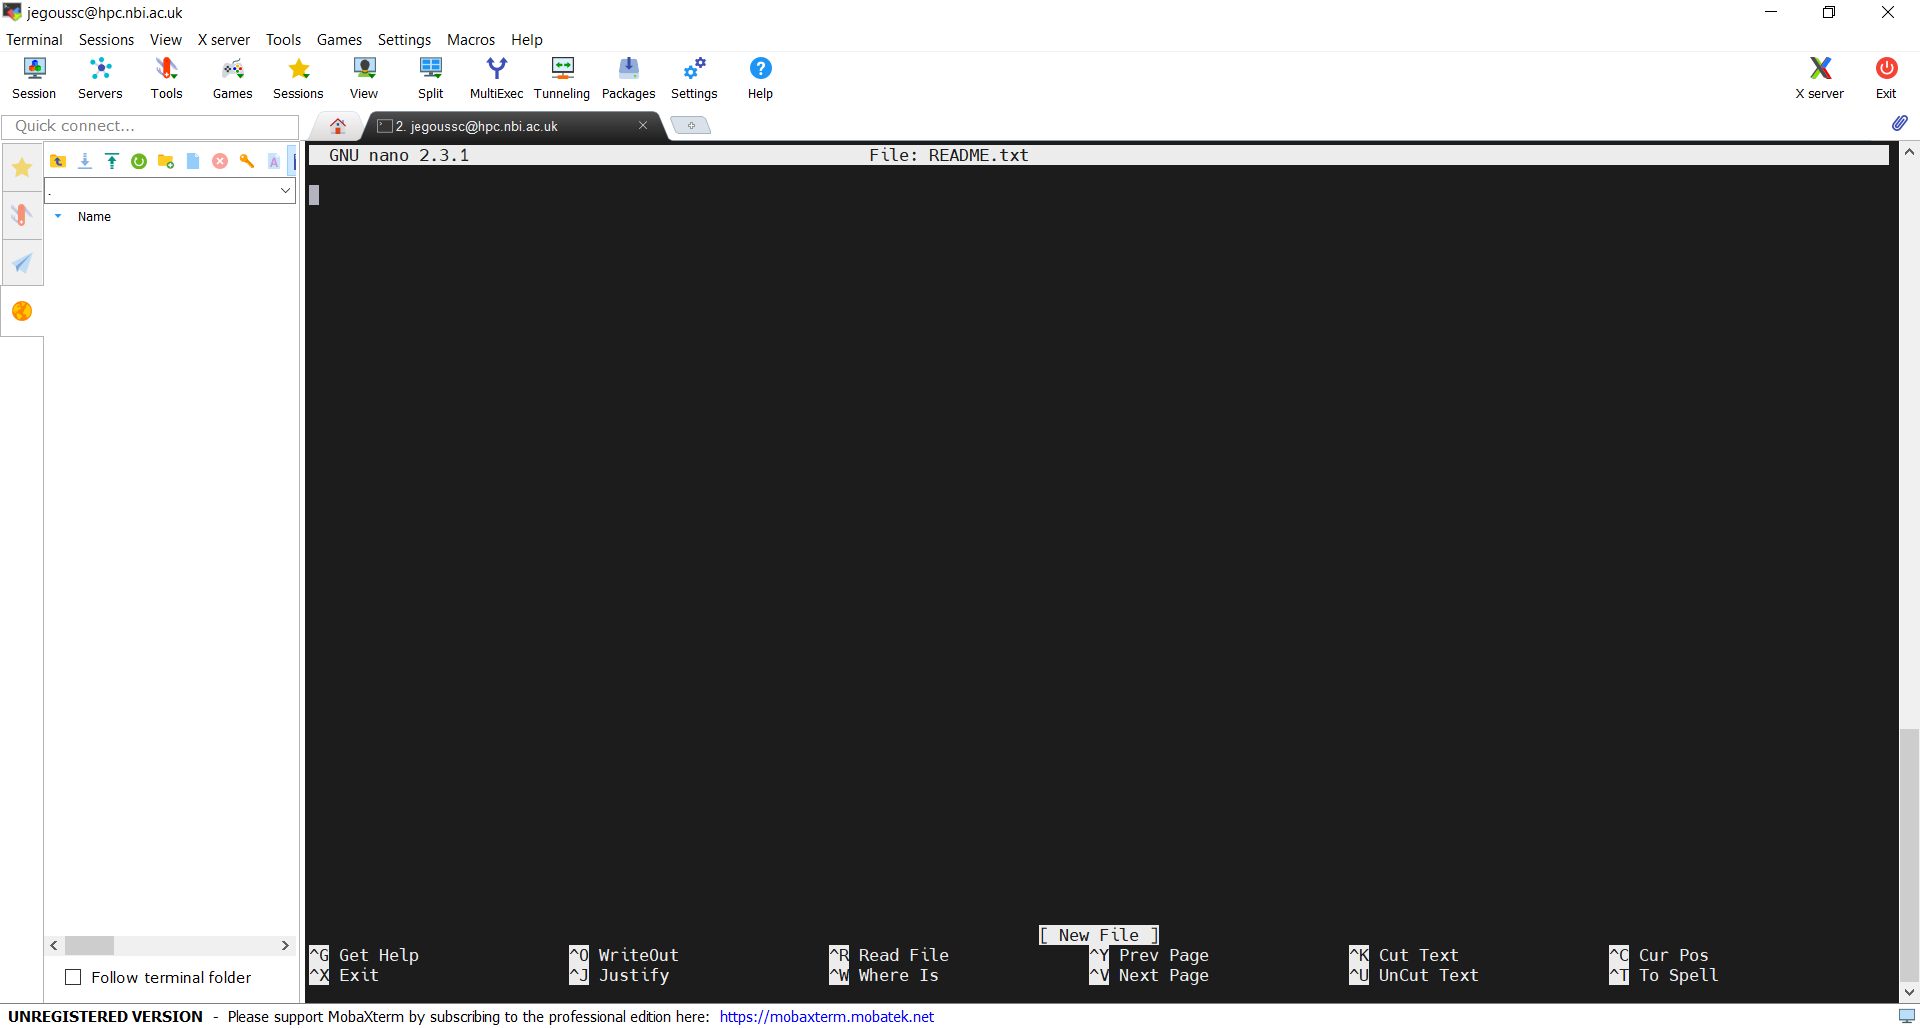
\includegraphics[keepaspectratio]{images/nano-mobaxterm.png}}

The text at the bottom of the screen shows the keyboard shortcuts for
performing various tasks in \texttt{nano}. We will talk more about how
to interpret this information soon.

\begin{tcolorbox}[enhanced jigsaw, opacitybacktitle=0.6, colback=white, coltitle=black, opacityback=0, rightrule=.15mm, toptitle=1mm, toprule=.15mm, bottomtitle=1mm, colframe=quarto-callout-note-color-frame, arc=.35mm, titlerule=0mm, colbacktitle=quarto-callout-note-color!10!white, leftrule=.75mm, title=\textcolor{quarto-callout-note-color}{\faInfo}\hspace{0.5em}{Which Editor?}, breakable, bottomrule=.15mm, left=2mm]

When we say, ``\texttt{nano} is a text editor,'' we really do mean
``text'': \texttt{nano} can only work with plain character data, not
tables, images, or any other human-friendly media. We use \texttt{nano}
in examples because it is one of the least complex text editors.
However, because of this trait, \texttt{nano} may not be powerful enough
or flexible enough for the work you need to do after this workshop. On
Unix systems (such as Linux and Mac OS X), many programmers use
\href{http://www.gnu.org/software/emacs/}{Emacs} or
\href{http://www.vim.org/}{Vim} (both of which require more time to
learn), or a graphical editor such as
\href{http://projects.gnome.org/gedit/}{Gedit}. On Windows, you may wish
to use \href{http://notepad-plus-plus.org/}{Notepad++}. Windows also has
a built-in editor called \texttt{notepad} that can be run from the
command line in the same way as \texttt{nano} for the purposes of this
lesson.

No matter what editor you use, you will need to know the default
location where it searches for files and where files are saved. If you
start an editor from the shell, it will (probably) use your current
working directory as its default location. If you use your computer's
start menu, the editor may want to save files in your desktop or
documents directory instead. You can change this by navigating to
another directory the first time you ``Save As\ldots{}''

\end{tcolorbox}

Let's type in a few lines of text. Describe what the files in this
directory are or what you've been doing with them. Once we're happy with
our text, we can press Ctrl-O (press the Ctrl or Control key and, while
holding it down, press the O key) to write our data to disk. You'll be
asked what file we want to save this to: press Return to accept the
suggested default of \texttt{README.txt}.

Once our file is saved, we can use Ctrl-X to quit the \texttt{nano}
editor and return to the shell.

The Control key is also called the ``Ctrl'' key. There are various ways
in which using the Control key may be described. For example, you may
see an instruction to press the Ctrl key and, while holding it down,
press the X key, described as any of:

\begin{itemize}
\tightlist
\item
  \texttt{Control-X}
\item
  \texttt{Control+X}
\item
  \texttt{Ctrl-X}
\item
  \texttt{Ctrl+X}
\item
  \texttt{\^{}X}
\item
  \texttt{C-x}
\end{itemize}

In \texttt{nano}, along the bottom of the screen you'll see
\texttt{\^{}G\ Get\ Help\ \^{}O\ WriteOut}. This means that you can use
Ctrl-G to get help and Ctrl-O to save your file.

Now you've written a file. You can take a look at it with \texttt{less}
or \texttt{cat}, or open it up again and edit it with \texttt{nano}.

\begin{tcolorbox}[enhanced jigsaw, opacitybacktitle=0.6, colback=white, coltitle=black, opacityback=0, rightrule=.15mm, toptitle=1mm, toprule=.15mm, bottomtitle=1mm, colframe=quarto-callout-caution-color-frame, arc=.35mm, titlerule=0mm, colbacktitle=quarto-callout-caution-color!10!white, leftrule=.75mm, title=\textcolor{quarto-callout-caution-color}{\faFire}\hspace{0.5em}{Exercise}, breakable, bottomrule=.15mm, left=2mm]

Open \texttt{README.txt} and add the date to the top of the file and
save the file.

\end{tcolorbox}

\begin{tcolorbox}[enhanced jigsaw, opacitybacktitle=0.6, colback=white, coltitle=black, opacityback=0, rightrule=.15mm, toptitle=1mm, toprule=.15mm, bottomtitle=1mm, colframe=quarto-callout-note-color-frame, arc=.35mm, titlerule=0mm, colbacktitle=quarto-callout-note-color!10!white, leftrule=.75mm, title=\textcolor{quarto-callout-note-color}{\faInfo}\hspace{0.5em}{Solution}, breakable, bottomrule=.15mm, left=2mm]

Use \texttt{nano\ README.txt} to open the file.\\
Add today's date and then use Ctrl-X followed by \texttt{y} and Enter to
save.

\end{tcolorbox}

\section{\texorpdfstring{\textbf{Writing
scripts}}{Writing scripts}}\label{writing-scripts}

A really powerful thing about the command line is that you can write
scripts. Scripts let you save commands to run them and also lets you put
multiple commands together. Though writing scripts may require an
additional time investment initially, this can save you time as you run
them repeatedly. Scripts can also address the challenge of
reproducibility: if you need to repeat an analysis, you retain a record
of your command history within the script.

One thing we will commonly want to do with sequencing results is pull
out bad reads and write them to a file to see if we can figure out
what's going on with them. We're going to look for reads with long
sequences of N's like we did before, but now we're going to write a
script, so we can run it each time we get new sequences, rather than
type the code in by hand each time.

We're going to create a new file to put this command in. We'll call it
\texttt{bad-reads-script.sh}. The \texttt{sh} isn't required, but using
that extension tells us that it's a shell script.

\begin{Shaded}
\begin{Highlighting}[]
\ExtensionTok{$}\NormalTok{ nano bad{-}reads{-}script.sh}
\end{Highlighting}
\end{Shaded}

Bad reads have a lot of N's, so we're going to look for
\texttt{NNNNNNNNNN} with \texttt{grep}. We want the whole FASTQ record,
so we're also going to get the one line above the sequence and the two
lines below. We also want to look in all the files that end with
\texttt{.fastq}, so we're going to use the \texttt{*} wildcard. We write
the following line in our script using \texttt{nano}:

\begin{verbatim}
grep -B1 -A2 -h NNNNNNNNNN *.fastq | grep -v '^--' > scripted_bad_reads.txt
\end{verbatim}

\begin{tcolorbox}[enhanced jigsaw, opacitybacktitle=0.6, colback=white, coltitle=black, opacityback=0, rightrule=.15mm, toptitle=1mm, toprule=.15mm, bottomtitle=1mm, colframe=quarto-callout-note-color-frame, arc=.35mm, titlerule=0mm, colbacktitle=quarto-callout-note-color!10!white, leftrule=.75mm, title=\textcolor{quarto-callout-note-color}{\faInfo}\hspace{0.5em}{Note}, breakable, bottomrule=.15mm, left=2mm]

We introduced the \texttt{-v} option, now we are using \texttt{-h} to
``Suppress the prefixing of file names on output'' according to the
documentation shown by \texttt{man\ grep}.

\end{tcolorbox}

Type your \texttt{grep} command into the file and save it as before. Be
careful that you did not add the \texttt{\$} at the beginning of the
line.

Quit \texttt{nano} by hitting \texttt{Ctrl} + \texttt{x} and \texttt{y}.

Now comes the neat part. We can run this script. Type:

\begin{Shaded}
\begin{Highlighting}[]
\ExtensionTok{$}\NormalTok{ bash bad{-}reads{-}script.sh}
\end{Highlighting}
\end{Shaded}

It will look like nothing happened, but now if you look at
\texttt{scripted\_bad\_reads.txt}, you can see that there are now reads
in the file.

\begin{tcolorbox}[enhanced jigsaw, opacitybacktitle=0.6, colback=white, coltitle=black, opacityback=0, rightrule=.15mm, toptitle=1mm, toprule=.15mm, bottomtitle=1mm, colframe=quarto-callout-caution-color-frame, arc=.35mm, titlerule=0mm, colbacktitle=quarto-callout-caution-color!10!white, leftrule=.75mm, title={Exercise}, breakable, bottomrule=.15mm, left=2mm]

We want the script to tell us when it's done.

\begin{enumerate}
\def\labelenumi{\arabic{enumi}.}
\item
  Open \texttt{bad-reads-script.sh} with \texttt{nano} and add the line
  \texttt{echo\ "Script\ finished!"} after the \texttt{grep} command and
  save the file.
\item
  Run the updated script.
\end{enumerate}

\end{tcolorbox}

\begin{tcolorbox}[enhanced jigsaw, opacitybacktitle=0.6, colback=white, coltitle=black, opacityback=0, rightrule=.15mm, toptitle=1mm, toprule=.15mm, bottomtitle=1mm, colframe=quarto-callout-caution-color-frame, arc=.35mm, titlerule=0mm, colbacktitle=quarto-callout-caution-color!10!white, leftrule=.75mm, title={Solution}, breakable, bottomrule=.15mm, left=2mm]

\begin{Shaded}
\begin{Highlighting}[]
\ExtensionTok{$}\NormalTok{ bash bad{-}reads{-}script.sh}
\ExtensionTok{Script}\NormalTok{ finished!}
\end{Highlighting}
\end{Shaded}

\end{tcolorbox}

\section{\texorpdfstring{\textbf{Making the script into a
program}}{Making the script into a program}}\label{making-the-script-into-a-program}

We had to type \texttt{bash} because we needed to tell the computer what
program to use to run this script. Instead, we can turn this script into
its own program. We need to tell the computer that this script is a
program by making the script file executable. We can do this by changing
the file permissions. We talked about permissions in
Chapter~\ref{sec-working-with-files-and-directories}.

First, let's look at the current permissions.

\begin{Shaded}
\begin{Highlighting}[]
\ExtensionTok{$}\NormalTok{ ls }\AttributeTok{{-}l}\NormalTok{ bad{-}reads{-}script.sh}
\ExtensionTok{{-}rwx{-}{-}{-}{-}{-}{-}}\NormalTok{ 1 }\PreprocessorTok{[}\SpecialStringTok{username}\PreprocessorTok{]}\NormalTok{ TSL\_20 100 Aug 11 14:38 bad{-}reads{-}script.sh}
\end{Highlighting}
\end{Shaded}

We see that it says \texttt{-rwx-\/-\/-\/-\/-\/-}. This shows that the
file can be read, modified and executed by you the file owner (you). We
want to change these permissions so that the file can be executed as a
program by anyone (groups and other users). We use the command
\texttt{chmod} like we did earlier when we removed write permissions.
Here we are adding (\texttt{+}) executable permissions (\texttt{+x}).

\begin{Shaded}
\begin{Highlighting}[]
\ExtensionTok{$}\NormalTok{ chmod +x bad{-}reads{-}script.sh}
\end{Highlighting}
\end{Shaded}

Now let's look at the permissions again.

\begin{Shaded}
\begin{Highlighting}[]
\ExtensionTok{$}\NormalTok{ ls }\AttributeTok{{-}l}\NormalTok{ bad{-}reads{-}script.sh}
\ExtensionTok{{-}rwx{-}{-}x{-}{-}x}\NormalTok{ 1 }\PreprocessorTok{[}\SpecialStringTok{username}\PreprocessorTok{]}\NormalTok{ TSL\_20 100 Aug 11 14:38 bad{-}reads{-}script.sh}
\end{Highlighting}
\end{Shaded}

Now we see that it says \texttt{-rwx–x-\/-x}. The \texttt{x}'s that are
there now tell us we can run it as a program. So, let's try it! We'll
need to put \texttt{./} at the beginning so the computer knows to look
here in this directory for the program.

\begin{verbatim}
$ ./bad-reads-script.sh
\end{verbatim}

The script should run the same way as before, but now we've created our
very own computer program!

You will learn more about writing scripts in a later lesson.

\section{\texorpdfstring{\textbf{Moving and Downloading
Data}}{Moving and Downloading Data}}\label{moving-and-downloading-data}

So far, we've worked with data that is already on the remote server.
Usually, however, most analyses begin with moving data onto your
directories on a server. Below we'll show you some commands to download
data onto your instance, or to move data between your computer and the
cloud.

\begin{tcolorbox}[enhanced jigsaw, opacitybacktitle=0.6, colback=white, coltitle=black, opacityback=0, rightrule=.15mm, toptitle=1mm, toprule=.15mm, bottomtitle=1mm, colframe=quarto-callout-warning-color-frame, arc=.35mm, titlerule=0mm, colbacktitle=quarto-callout-warning-color!10!white, leftrule=.75mm, title=\textcolor{quarto-callout-warning-color}{\faExclamationTriangle}\hspace{0.5em}{No internet on HPC}, breakable, bottomrule=.15mm, left=2mm]

The HPC is not connected to the internet for security reasons so you
must log out of the HPC to download files on your own device. Then the
files can be transferred to the HPC.

\begin{Shaded}
\begin{Highlighting}[]
\ExtensionTok{$}\NormalTok{ logout}
\ExtensionTok{Connection}\NormalTok{ to hpc.nbi.ac.uk closed.}
\end{Highlighting}
\end{Shaded}

\end{tcolorbox}

\subsection{\texorpdfstring{\textbf{Getting data from the
cloud}}{Getting data from the cloud}}\label{getting-data-from-the-cloud}

There are two programs that will download data from a remote server to
your local (or remote) machine: \texttt{wget} and \texttt{curl}. They
were designed to do slightly different tasks by default, so you'll need
to give the programs somewhat different options to get the same
behaviour, but they are mostly interchangeable.

\begin{itemize}
\item
  \texttt{wget} is short for ``world wide web get'', and it's basic
  function is to \emph{download} web pages or data at a web address.
\item
  \texttt{curl} is a pun, it is supposed to be read as ``see URL'', so
  its basic function is to \emph{display} webpages or data at a web
  address.
\end{itemize}

Which one you need to use mostly depends on your operating system, as
most computers will only have one or the other installed by default.

Let's say you want to download some data from Ensembl. We're going to
download a very small tab-delimited file that just tells us what data is
available on the Ensembl bacteria server. Before we can start our
download, we need to know whether we're using \texttt{curl} or
\texttt{wget}.

To see which program you have, type:

\begin{Shaded}
\begin{Highlighting}[]
\ExtensionTok{$}\NormalTok{ which curl}
\ExtensionTok{$}\NormalTok{ which wget}
\end{Highlighting}
\end{Shaded}

\texttt{which} is a BASH program that looks through everything you have
installed, and tells you what folder it is installed to. If it can't
find the program you asked for, it returns nothing, i.e.~gives you no
results.

On Mac OSX, you'll likely get the following output:

\begin{Shaded}
\begin{Highlighting}[]
\ExtensionTok{$}\NormalTok{ which curl}
\ExtensionTok{/usr/bin/curl}
\end{Highlighting}
\end{Shaded}

\begin{Shaded}
\begin{Highlighting}[]
\ExtensionTok{$}\NormalTok{ which wget}
\ExtensionTok{$}
\end{Highlighting}
\end{Shaded}

This output means that you have \texttt{curl} installed, but not
\texttt{wget}.

Once you know whether you have \texttt{curl} or \texttt{wget}, use one
of the following commands to download the file:

\begin{Shaded}
\begin{Highlighting}[]
\ExtensionTok{$}\NormalTok{ cd MyDocuments  }\CommentTok{\# directory on your local machine}
\ExtensionTok{$}\NormalTok{ wget ftp://ftp.ensemblgenomes.org/pub/release{-}37/bacteria/species\_EnsemblBacteria.txt}
\end{Highlighting}
\end{Shaded}

or

\begin{Shaded}
\begin{Highlighting}[]
\ExtensionTok{$}\NormalTok{ cd MyDocuments}
\ExtensionTok{$}\NormalTok{ curl }\AttributeTok{{-}O}\NormalTok{ ftp://ftp.ensemblgenomes.org/pub/release{-}37/bacteria/species\_EnsemblBacteria.txt}
\end{Highlighting}
\end{Shaded}

Since we wanted to \emph{download} the file rather than just view it, we
used \texttt{wget} without any modifiers. With \texttt{curl} however, we
had to use the -O flag, which simultaneously tells \texttt{curl} to
download the page instead of showing it to us \textbf{and} specifies
that it should save the file using the same name it had on the server:
species\_EnsemblBacteria.txt

It's important to note that both \texttt{curl} and \texttt{wget}
download to the computer that the command line belongs to. So, if you
are logged into AWS on the command line and execute the \texttt{curl}
command above in the AWS terminal, the file will be downloaded to your
AWS machine, not your local one.

\subsection{\texorpdfstring{\textbf{Moving files between your laptop and
the
server}}{Moving files between your laptop and the server}}\label{moving-files-between-your-laptop-and-the-server}

It is possible to access the NBI server using the Windows navigation
system. To do so, you must map the network drive:

\begin{enumerate}
\def\labelenumi{\arabic{enumi}.}
\tightlist
\item
  Access your computer (by clicking on the computer icon on your
  desktop) .
\item
  Under the ``Computer'' tab, use the pull-down menu ``Map network
  drive'' and select ``Map network drive''. This will open a pop-up
  window asking what network drive you would like to map
\item
  Under ``Folder'' enter
  \texttt{\textbackslash{}\textbackslash{}tsl-hpc-data\textbackslash{}HPC-Home}
  and click ``Finish''.
\item
  You now have access to HPC-Home through the Windows navigation system.
\end{enumerate}

\begin{figure}

\begin{minipage}{0.50\linewidth}

\pandocbounded{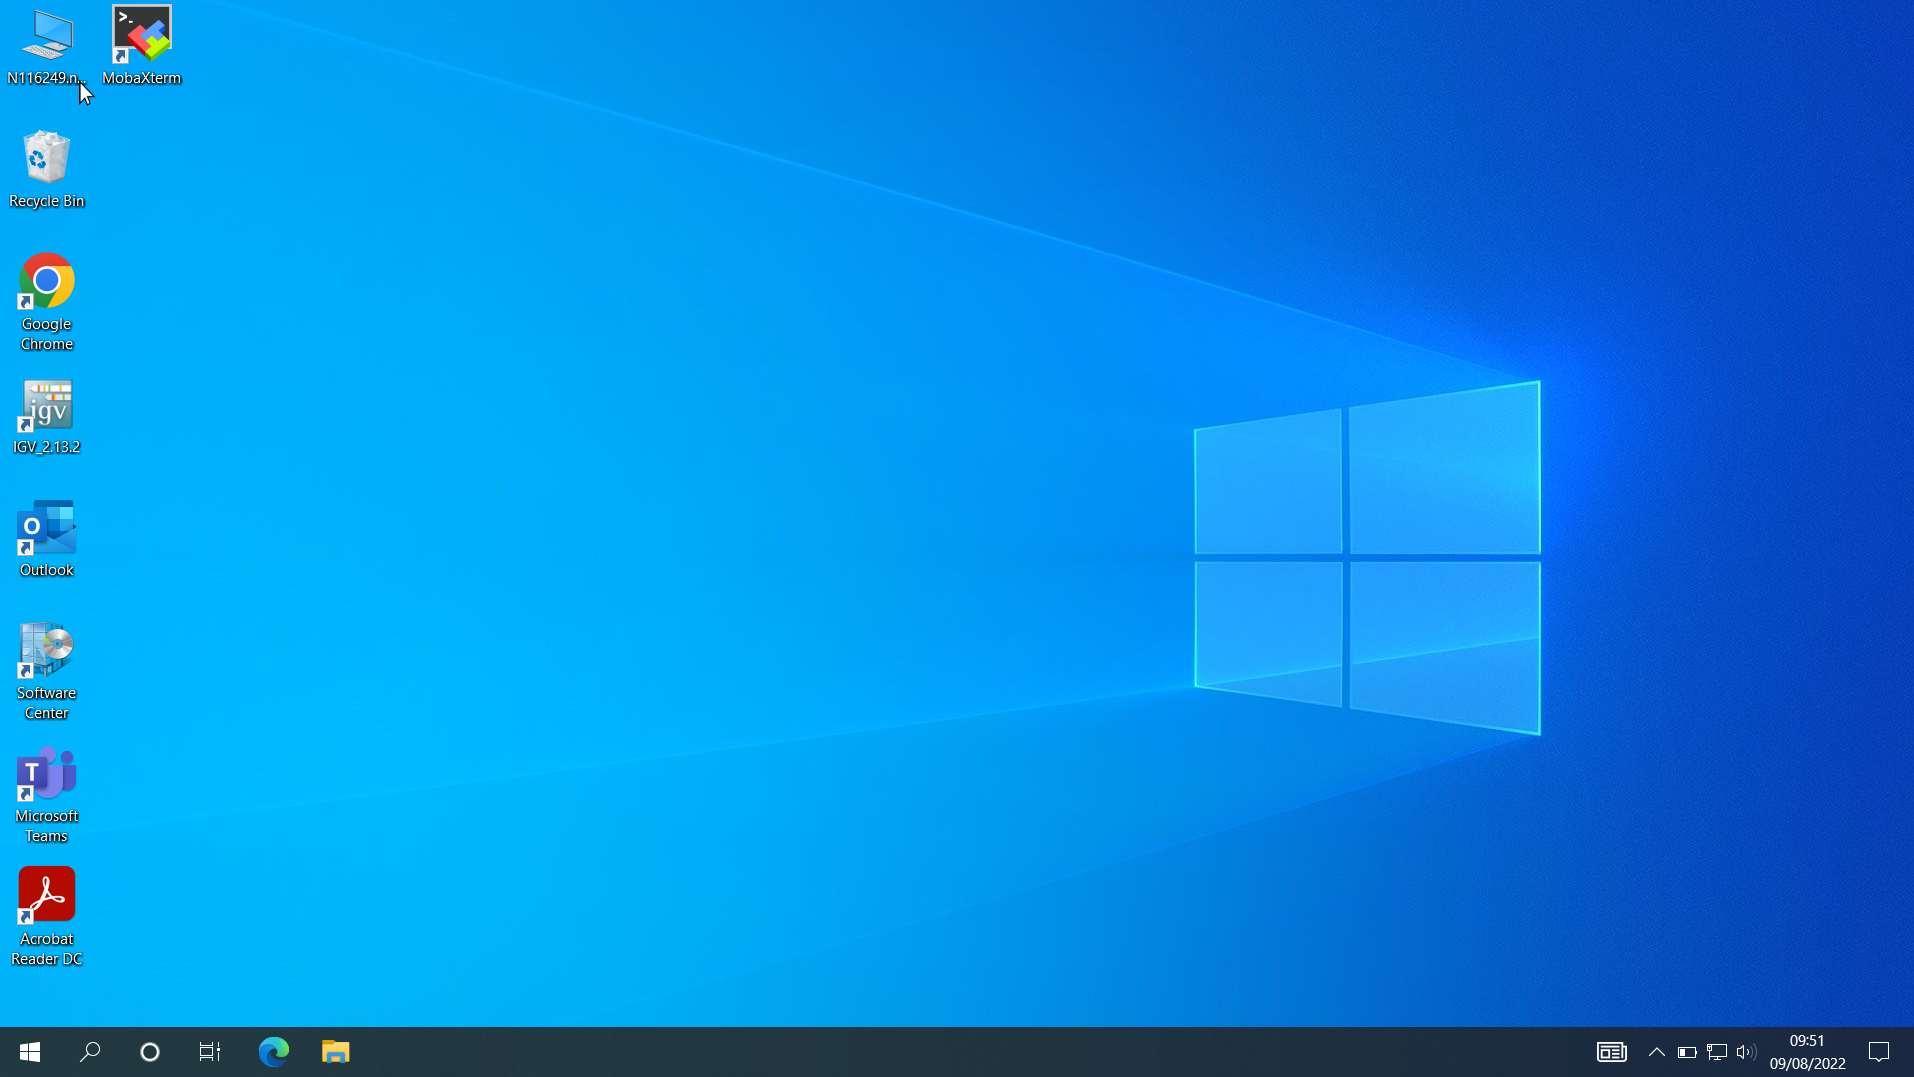
\includegraphics[keepaspectratio]{images/desktop.png}}

\subcaption{\label{}Step 1}
\end{minipage}%
%
\begin{minipage}{0.50\linewidth}

\pandocbounded{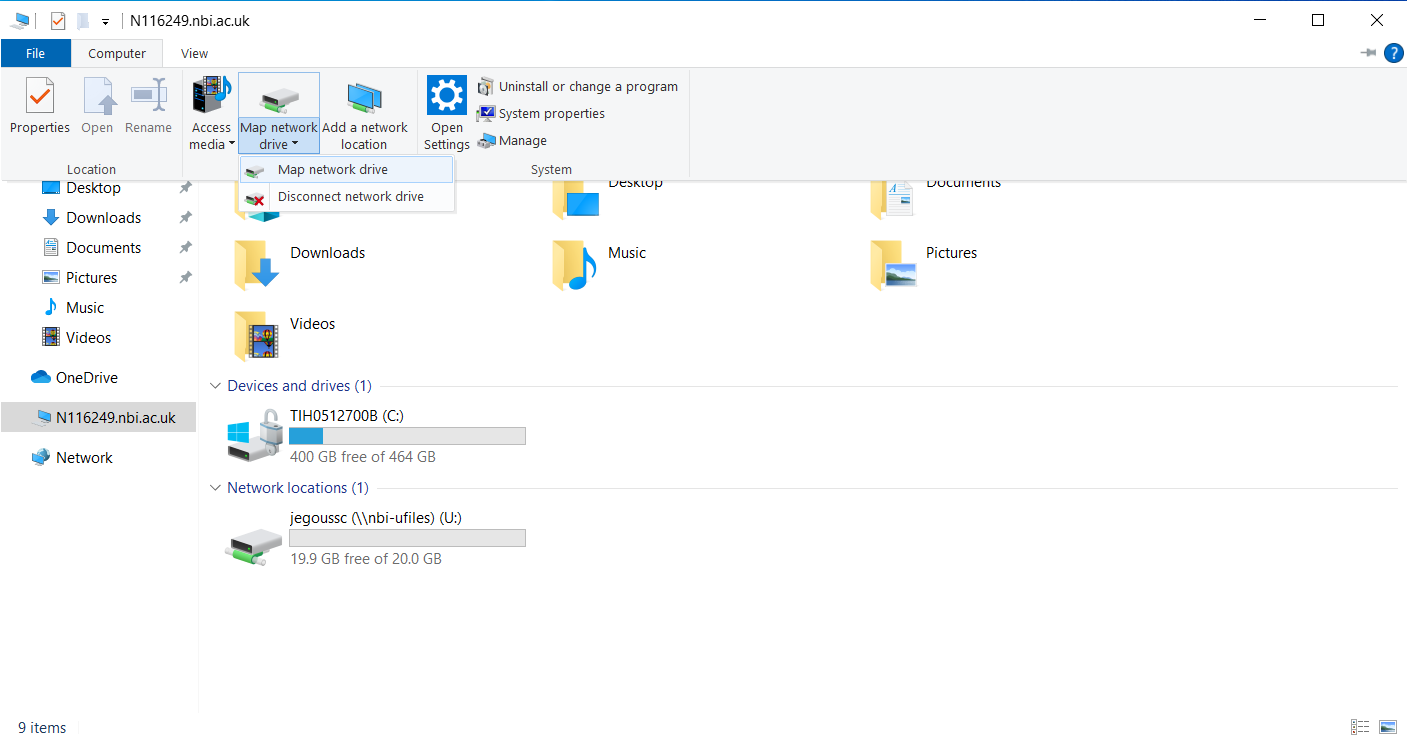
\includegraphics[keepaspectratio]{images/computer04.png}}

\subcaption{\label{}Step 2}
\end{minipage}%
\newline
\begin{minipage}{0.50\linewidth}

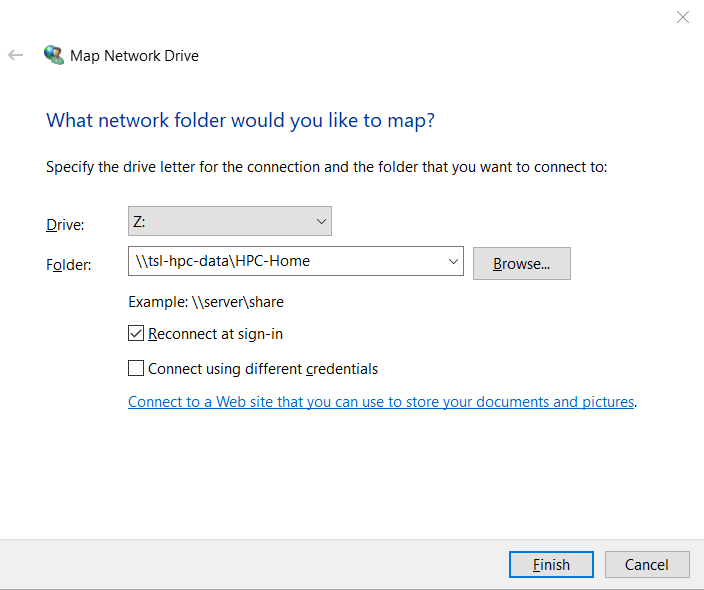
\includegraphics[width=5.20833in,height=\textheight,keepaspectratio]{images/network02.png}

\subcaption{\label{}Step 3}
\end{minipage}%
%
\begin{minipage}{0.50\linewidth}

\pandocbounded{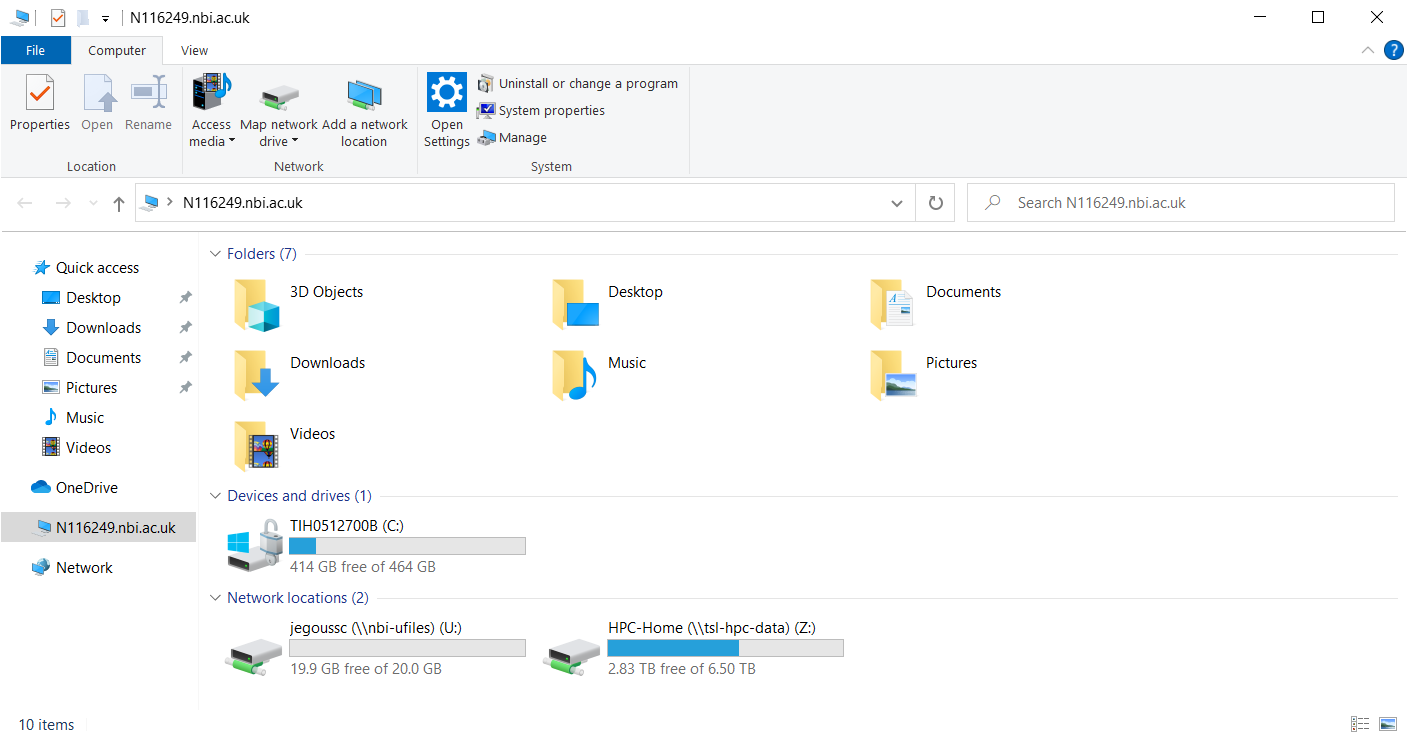
\includegraphics[keepaspectratio]{images/access-hpc.png}}

\subcaption{\label{}Step 4}
\end{minipage}%

\caption{\label{fig-access-hpc}Screen captures of the steps to map
network drive.}

\end{figure}%

\section{Summary}\label{summary-4}

\begin{tcolorbox}[enhanced jigsaw, opacitybacktitle=0.6, colback=white, coltitle=black, opacityback=0, rightrule=.15mm, toptitle=1mm, toprule=.15mm, bottomtitle=1mm, colframe=quarto-callout-important-color-frame, arc=.35mm, titlerule=0mm, colbacktitle=quarto-callout-important-color!10!white, leftrule=.75mm, title=\textcolor{quarto-callout-important-color}{\faExclamation}\hspace{0.5em}{Key points}, breakable, bottomrule=.15mm, left=2mm]

\begin{itemize}
\tightlist
\item
  Scripts are a collection of commands executed together.
\item
  Transferring information to and from virtual and local computers.
\end{itemize}

\end{tcolorbox}

\bookmarksetup{startatroot}

\chapter{Organisation}\label{sec-organisation}

\begin{tcolorbox}[enhanced jigsaw, opacitybacktitle=0.6, colback=white, coltitle=black, opacityback=0, rightrule=.15mm, toptitle=1mm, toprule=.15mm, bottomtitle=1mm, colframe=quarto-callout-note-color-frame, arc=.35mm, titlerule=0mm, colbacktitle=quarto-callout-note-color!10!white, leftrule=.75mm, title={⏳ Time}, breakable, bottomrule=.15mm, left=2mm]

\begin{itemize}
\tightlist
\item
  Teaching: 15 min
\item
  Exercises: 15 min
\end{itemize}

\end{tcolorbox}

\begin{tcolorbox}[enhanced jigsaw, opacitybacktitle=0.6, colback=white, coltitle=black, opacityback=0, rightrule=.15mm, toptitle=1mm, toprule=.15mm, bottomtitle=1mm, colframe=quarto-callout-tip-color-frame, arc=.35mm, titlerule=0mm, colbacktitle=quarto-callout-tip-color!10!white, leftrule=.75mm, title={🤔 Questions}, breakable, bottomrule=.15mm, left=2mm]

\begin{itemize}
\tightlist
\item
  How can I organize my file system for a new bioinformatics project?
\item
  How can I document my work?
\end{itemize}

\end{tcolorbox}

\begin{tcolorbox}[enhanced jigsaw, opacitybacktitle=0.6, colback=white, coltitle=black, opacityback=0, rightrule=.15mm, toptitle=1mm, toprule=.15mm, bottomtitle=1mm, colframe=quarto-callout-important-color-frame, arc=.35mm, titlerule=0mm, colbacktitle=quarto-callout-important-color!10!white, leftrule=.75mm, title={🎯 Objectives}, breakable, bottomrule=.15mm, left=2mm]

\begin{itemize}
\tightlist
\item
  Create a file system for a bioinformatics project.
\item
  Explain what types of files should go in your docs, data, and results
  directories.
\item
  Use the history command and a text editor like nano to document your
  work on your project.
\end{itemize}

\end{tcolorbox}

\section{Getting your project
started}\label{getting-your-project-started}

Project organization is one of the most important parts of a sequencing
project, and yet is often overlooked amidst the excitement of getting a
first look at new data. Of course, while it's best to get yourself
organized before you even begin your analyses, it's never too late to
start, either.

You should approach your sequencing project similarly to how you do a
biological experiment and this ideally begins with experimental design.
We're going to assume that you've already designed a beautiful
sequencing experiment to address your biological question, collected
appropriate samples, and that you have enough statistical power to
answer the questions you're interested in asking. These steps are all
incredibly important, but beyond the scope of our course. For all of
those steps (collecting specimens, extracting DNA, prepping your
samples) you've likely kept a lab notebook that details how and why you
did each step. However, the process of documentation doesn't stop at the
sequencer!

Genomics projects can quickly accumulate hundreds of files across tens
of folders. Every computational analysis you perform over the course of
your project is going to create many files, which can especially become
a problem when you'll inevitably want to run some of those analyses
again. For instance, you might have made significant headway into your
project, but then have to remember the PCR conditions you used to create
your sequencing library months prior.

Other questions might arise along the way:

\begin{itemize}
\item
  What were your best alignment results?
\item
  Which folder were they in: Analysis1, AnalysisRedone, Analysis1a, or
  AnalysisRedone2?
\item
  Which quality cutoff did you use?
\item
  What version of a given program did you implement your analysis in?
\end{itemize}

Good documentation is key to avoiding this issue, and luckily enough,
recording your computational experiments is even easier than recording
lab data. Copy/Paste will become your best friend, sensible file names
will make your analysis understandable by you and your collaborators,
and writing the methods section for your next paper will be easy!
Remember that in any given project of yours, it's worthwhile to consider
a future version of yourself as an entirely separate collaborator. The
better your documentation is, the more this `collaborator' will feel
indebted to you!

With this in mind, let's have a look at the best practices for
documenting your genomics project. Your future self will thank you.

In this exercise we will setup a file system for the project we will be
working on during this workshop.

\begin{tcolorbox}[enhanced jigsaw, opacitybacktitle=0.6, colback=white, coltitle=black, opacityback=0, rightrule=.15mm, toptitle=1mm, toprule=.15mm, bottomtitle=1mm, colframe=quarto-callout-warning-color-frame, arc=.35mm, titlerule=0mm, colbacktitle=quarto-callout-warning-color!10!white, leftrule=.75mm, title=\textcolor{quarto-callout-warning-color}{\faExclamationTriangle}\hspace{0.5em}{Warning}, breakable, bottomrule=.15mm, left=2mm]

Make sure you are connected to the remote server:

\begin{Shaded}
\begin{Highlighting}[]
\ExtensionTok{$}\NormalTok{ ssh }\PreprocessorTok{[}\SpecialStringTok{username}\PreprocessorTok{]}\NormalTok{@hpc.nbi.ac.uk}
\end{Highlighting}
\end{Shaded}

\end{tcolorbox}

We will start by creating a directory that we can use for the rest of
the workshop. First navigate to your home directory. Then confirm that
you are in the correct directory using the \texttt{pwd} command.

\begin{Shaded}
\begin{Highlighting}[]
\ExtensionTok{$}\NormalTok{ cd}
\ExtensionTok{$}\NormalTok{ pwd}
\ExtensionTok{/hpc{-}home/[username]/}
\end{Highlighting}
\end{Shaded}

\begin{tcolorbox}[enhanced jigsaw, opacitybacktitle=0.6, colback=white, coltitle=black, opacityback=0, rightrule=.15mm, toptitle=1mm, toprule=.15mm, bottomtitle=1mm, colframe=quarto-callout-caution-color-frame, arc=.35mm, titlerule=0mm, colbacktitle=quarto-callout-caution-color!10!white, leftrule=.75mm, title={Exercise}, breakable, bottomrule=.15mm, left=2mm]

Use the command like to make the following directories:

\begin{itemize}
\tightlist
\item
  \texttt{dc\_workshop}
\item
  \texttt{dc\_workshop/docs}
\item
  \texttt{dc\_workshop/data}
\item
  \texttt{dc\_workshop/results}
\end{itemize}

\end{tcolorbox}

\begin{tcolorbox}[enhanced jigsaw, opacitybacktitle=0.6, colback=white, coltitle=black, opacityback=0, rightrule=.15mm, toptitle=1mm, toprule=.15mm, bottomtitle=1mm, colframe=quarto-callout-caution-color-frame, arc=.35mm, titlerule=0mm, colbacktitle=quarto-callout-caution-color!10!white, leftrule=.75mm, title={Solution}, breakable, bottomrule=.15mm, left=2mm]

\begin{Shaded}
\begin{Highlighting}[]
\ExtensionTok{$}\NormalTok{ mkdir dc\_workshop}
\ExtensionTok{$}\NormalTok{ mkdir dc\_workshop/docs}
\ExtensionTok{$}\NormalTok{ mkdir dc\_workshop/data}
\ExtensionTok{$}\NormalTok{ mkdir dc\_workshop/results}
\end{Highlighting}
\end{Shaded}

\end{tcolorbox}

Use \texttt{ls\ -R} to verify that you have created these directories.
The \texttt{-R} option for \texttt{ls} stands for recursive. This option
causes \texttt{ls} to return the contents of each subdirectory within
the directory iteratively.

\begin{Shaded}
\begin{Highlighting}[]
\ExtensionTok{$}\NormalTok{ ls }\AttributeTok{{-}R}\NormalTok{ dc\_workshop}
\ExtensionTok{dc\_workshop/:}
\ExtensionTok{data}\NormalTok{  docs  results}

\ExtensionTok{dc\_workshop/data:}

\ExtensionTok{dc\_workshop/docs:}

\ExtensionTok{dc\_workshop/results:} 
\end{Highlighting}
\end{Shaded}

\section{Organizing your files}\label{organizing-your-files}

Before beginning any analysis, it's important to save a copy of your raw
data. The raw data should never be changed. Regardless of how sure you
are that you want to carry out a particular data cleaning step, there's
always the chance that you'll change your mind later or that there will
be an error in carrying out the data cleaning and you'll need to go back
a step in the process. Having a raw copy of your data that you never
modify guarantees that you will always be able to start over if
something goes wrong with your analysis. When starting any analysis, you
can make a copy of your raw data file and do your manipulations on that
file, rather than the raw version. We learned previously (in
Section~\ref{sec-file-permissions}) how to prevent overwriting our raw
data files by setting restrictive file permissions.

You can store any results that are generated from your analysis in the
\texttt{results} folder. This guarantees that you won't confuse results
file and data files in six months or two years when you are looking back
through your files in preparation for publishing your study.

The \texttt{docs} folder is the place to store any written analysis of
your results, notes about how your analyses were carried out, and
documents related to your eventual publication.

\section{Documenting your activity on the
project}\label{documenting-your-activity-on-the-project}

When carrying out wet-lab analyses, most scientists work from a written
protocol and keep a hard copy of written notes in their lab notebook,
including any things they did differently from the written protocol.
This detailed record-keeping process is just as important when doing
computational analyses. Luckily, it's even easier to record the steps
you've carried out computational than it is when working at the bench.

The \texttt{history} command is a convenient way to document all the
commands you have used while analyzing and manipulating your project
files. Let's document the work we have done on our project so far.

View the commands that you have used so far during this session using
\texttt{history}:

\begin{Shaded}
\begin{Highlighting}[]
\ExtensionTok{$}\NormalTok{ history}
\end{Highlighting}
\end{Shaded}

The history likely contains many more commands than you have used for
the current project. Let's view the last several commands that focus on
just what we need for this project.

View the last n lines of your history (where n = approximately the last
few lines you think relevant). For our example, we will use the last 7:

\begin{Shaded}
\begin{Highlighting}[]
\ExtensionTok{$}\NormalTok{ history }\KeywordTok{|} \FunctionTok{tail} \AttributeTok{{-}n}\NormalTok{ 7}
\end{Highlighting}
\end{Shaded}

\begin{tcolorbox}[enhanced jigsaw, opacitybacktitle=0.6, colback=white, coltitle=black, opacityback=0, rightrule=.15mm, toptitle=1mm, toprule=.15mm, bottomtitle=1mm, colframe=quarto-callout-caution-color-frame, arc=.35mm, titlerule=0mm, colbacktitle=quarto-callout-caution-color!10!white, leftrule=.75mm, title={Exercise}, breakable, bottomrule=.15mm, left=2mm]

Using your knowledge of the shell, use the append redirect
\texttt{\textgreater{}\textgreater{}} to create a file called
\texttt{dc\_workshop\_log\_XXXX\_XX\_XX.sh} (Use the four-digit year,
two-digit month, and two digit day,
e.g.~\texttt{dc\_workshop\_log\_2021\_10\_27.sh})

\end{tcolorbox}

\begin{tcolorbox}[enhanced jigsaw, opacitybacktitle=0.6, colback=white, coltitle=black, opacityback=0, rightrule=.15mm, toptitle=1mm, toprule=.15mm, bottomtitle=1mm, colframe=quarto-callout-caution-color-frame, arc=.35mm, titlerule=0mm, colbacktitle=quarto-callout-caution-color!10!white, leftrule=.75mm, title={Solution}, breakable, bottomrule=.15mm, left=2mm]

\begin{Shaded}
\begin{Highlighting}[]
\ExtensionTok{$}\NormalTok{ history }\KeywordTok{|} \FunctionTok{tail} \AttributeTok{{-}n}\NormalTok{ 7 }\OperatorTok{\textgreater{}\textgreater{}}\NormalTok{ dc\_workshop\_log\_2022\_10\_20.sh}
\end{Highlighting}
\end{Shaded}

Note we used the last 7 lines as an example, the number of lines may
vary.

\end{tcolorbox}

You may have noticed that your history contains the \texttt{history}
command itself. To remove this redundancy from our log, let's use the
\texttt{nano} text editor to fix the file:

\begin{Shaded}
\begin{Highlighting}[]
\ExtensionTok{$}\NormalTok{ nano dc\_workshop\_log\_2022\_10\_20.sh}
\end{Highlighting}
\end{Shaded}

\begin{tcolorbox}[enhanced jigsaw, opacitybacktitle=0.6, colback=white, coltitle=black, opacityback=0, rightrule=.15mm, toptitle=1mm, toprule=.15mm, bottomtitle=1mm, colframe=quarto-callout-tip-color-frame, arc=.35mm, titlerule=0mm, colbacktitle=quarto-callout-tip-color!10!white, leftrule=.75mm, title=\textcolor{quarto-callout-tip-color}{\faLightbulb}\hspace{0.5em}{Navigating in Nano}, breakable, bottomrule=.15mm, left=2mm]

Although \texttt{nano} is useful, it can be frustrating to edit
documents, as you can't use your mouse to navigate to the part of the
document you would like to edit. Here are some useful keyboard shortcuts
for moving around within a text document in \texttt{nano}. You can find
more information by typing Ctrl-G within \texttt{nano}.

\begin{longtable}[]{@{}
  >{\raggedright\arraybackslash}p{(\linewidth - 2\tabcolsep) * \real{0.4306}}
  >{\raggedright\arraybackslash}p{(\linewidth - 2\tabcolsep) * \real{0.5694}}@{}}
\toprule\noalign{}
\begin{minipage}[b]{\linewidth}\raggedright
key
\end{minipage} & \begin{minipage}[b]{\linewidth}\raggedright
action
\end{minipage} \\
\midrule\noalign{}
\endhead
\bottomrule\noalign{}
\endlastfoot
Ctrl-Space OR Ctrl-→ & to move forward one word \\
Alt-Space OR Esc-Space OR Ctrl-← & to move back one word \\
Ctrl-A & to move to the beginning of the current line \\
Ctrl-E & to move to the end of the current line \\
Ctrl-W & to search \\
\end{longtable}

\end{tcolorbox}

Add a date line and comment to the line where you have created the
directory. Recall that any text on a line after a \texttt{\#} is ignored
by bash when evaluating the text as code. For example:

\begin{verbatim}
# 2022_10_20   
# Created sample directories for the course
\end{verbatim}

Next, remove any lines of the history that are not relevant by
navigating to those lines and using your delete key. Save your file and
close \texttt{nano}.

Your file should look something like this:

\begin{verbatim}
# 2022_10_20   
# Created sample directories for the course

mkdir dc_workshop
mkdir dc_workshop/docs
mkdir dc_workshop/data
mkdir dc_workshop/results
\end{verbatim}

If you keep this file up to date, you can use it to re-do your work on
your project if something happens to your results files. To demonstrate
how this works, first delete your \texttt{dc\_workshop} directory and
all of its subdirectories. Look at your directory contents to verify the
directory is gone.

\begin{Shaded}
\begin{Highlighting}[]
\ExtensionTok{$}\NormalTok{ rm }\AttributeTok{{-}r}\NormalTok{ dc\_workshop}
\ExtensionTok{$}\NormalTok{ ls}
\ExtensionTok{shell\_data}\NormalTok{  dc\_workshop\_log\_2022\_10\_20.sh}
\end{Highlighting}
\end{Shaded}

\begin{Shaded}
\begin{Highlighting}[]
\ExtensionTok{$}\NormalTok{ bash dc\_workshop\_log\_2017\_10\_27.sh}
\ExtensionTok{$}\NormalTok{ ls}
\ExtensionTok{shell\_data}\NormalTok{  dc\_workshop dc\_workshop\_log\_2017\_10\_27.sh}
\end{Highlighting}
\end{Shaded}

It's important that we keep our workshop log file outside of our
\texttt{dc\_workshop} directory if we want to use it to recreate our
work. It's also important for us to keep it up to date by regularly
updating with the commands that we used to generate our results files.

Congratulations! You've finished your introduction to using the shell
for genomics projects. You now know how to navigate your file system,
create, copy, move, and remove files and directories, and automate
repetitive tasks using scripts and wildcards. With this solid
foundation, you're ready to move on to apply all of these new skills to
carrying out more sophisticated bioinformatics analysis work. Don't
worry if everything doesn't feel perfectly comfortable yet. We're going
to have many more opportunities for practice as we move forward on our
bioinformatics journey!

\section{Summary}\label{summary-5}

\begin{tcolorbox}[enhanced jigsaw, opacitybacktitle=0.6, colback=white, coltitle=black, opacityback=0, rightrule=.15mm, toptitle=1mm, toprule=.15mm, bottomtitle=1mm, colframe=quarto-callout-important-color-frame, arc=.35mm, titlerule=0mm, colbacktitle=quarto-callout-important-color!10!white, leftrule=.75mm, title=\textcolor{quarto-callout-important-color}{\faExclamation}\hspace{0.5em}{Key points}, breakable, bottomrule=.15mm, left=2mm]

\begin{itemize}
\tightlist
\item
  Spend the time to organize your file system when you start a new
  project. Your future self will thank you!
\item
  Always save a write-protected copy of your raw data.
\end{itemize}

\end{tcolorbox}

If you want to read more about how to organise your project, you can
read the
\href{http://journals.plos.org/ploscompbiol/article?id=10.1371/journal.pcbi.1000424}{Quick
Guide to Organizing Computational Biology Projects} (Noble 2009).

\bookmarksetup{startatroot}

\chapter*{References}\label{references}
\addcontentsline{toc}{chapter}{References}

\markboth{References}{References}

\phantomsection\label{refs}
\begin{CSLReferences}{1}{0}
\bibitem[\citeproctext]{ref-becker2019genomics}
Becker, Erin Alison, Anita Schürch, Tracy Teal, Sheldon John McKay,
Jessica Elizabeth Mizzi, François Michonneau, Amy E. Hodge, et al. 2019.
{``{datacarpentry/shell-genomics: Data Carpentry: Introduction to the
shell for genomics data, June 2019}.''} Zenodo.
\url{https://doi.org/10.5281/zenodo.3260560}.

\bibitem[\citeproctext]{ref-noble2009organization}
Noble, William Stafford. 2009. {``A Quick Guide to Organizing
Computational Biology Projects.''} \emph{PLOS Computational Biology} 5
(7): 1--5. \url{https://doi.org/10.1371/journal.pcbi.1000424}.

\end{CSLReferences}




\end{document}
